\documentclass[a4paper,10pt]{article}
\usepackage[utf8]{inputenc}

% ----  Useful packages % ---- 
\usepackage{amsmath}
\usepackage{graphicx}
\usepackage{amsfonts}
\usepackage{amsthm}
\usepackage{amssymb}
% ----  Useful packages % ---- 

\usepackage{wrapfig}
\usepackage{caption}
\usepackage{subcaption}

\usepackage{hyperref}
\hypersetup{
    colorlinks,
    citecolor=black,
    filecolor=black,
    linkcolor=black,
    urlcolor=black
}

\graphicspath{ {./images/} }

% ---- Set page size and margins replace ------
\usepackage[letterpaper,top=2cm,bottom=2cm,left=3cm,right=3cm,marginparwidth=1.75cm]{geometry}
% ---- Set page size and margins replace ------

% ---- Definition of custum section ---- 
\newtheorem{note}{Note}[subsection]
\newtheorem{definition}{Definizione}[section]

\theoremstyle{definition}
\newtheorem{example}{Esempio}[section]

\theoremstyle{definition}
\newtheorem{demostration}{Dimotrazione}[section]

\theoremstyle{plain}
\newtheorem{proposition}{Proposizione}[section]

\theoremstyle{plain}
\newtheorem{theorem}{Teorema}[section]

\theoremstyle{plain}
\newtheorem{lemma}{Lemma}[section]

\theoremstyle{plain}
\newtheorem{corollar}{Corollario}[section]
% ---- Definition of custum section ---- 

% ---- Footer and header ---- 
\usepackage{fancyhdr}
\pagestyle{fancy}
\fancyhf{}
\fancyhead[LE,RO]{A.A 2022-2023}
\fancyhead[RE,LO]{Fondamenti d'informatica}
\fancyfoot[RE,LO]{\rightmark}
\fancyfoot[LE,RO]{\thepage}

\renewcommand{\headrulewidth}{.5pt}
\renewcommand{\footrulewidth}{.5pt}
% ---- Footer and header ---- 

% ----  Language setting ---- 
\usepackage[italian, english]{babel}
% ----  Language setting ---- 


\title{\textbf{Fondamenti d'informatica}}
\author{Realizzato da: Giuntoni Matteo}
\date{A.A 2022-2023}

\begin{document}
\begin{titlepage} %crea l'enviroment
	\begin{figure}[t] %inserisce le figure
		\centering
\includegraphics[width=0.98\textwidth]{marchio_unipi_pant541.png}
	\end{figure}
	\vspace{20mm}
	
	\begin{Large}
		\begin{center}
			\textbf{Dipartimento di Informatica\\ Corso di Laurea Triennale in Informatica\\}
			\vspace{20mm}
			{\LARGE{Corso a Libera Scelta - 6 CFU}}\\
			\vspace{10mm}
			{\huge{\bf Computer Graphics}}\\
		\end{center}
	\end{Large}
	
	
	\vspace{36mm}
	%minipage divide la pagina in due sezioni settabili
	\begin{minipage}[t]{0.47\textwidth}
		{\large{\bf Professore:}\\ \large{Prof. }}
	\end{minipage}
	\hfill
	\begin{minipage}[t]{0.47\textwidth}\raggedleft
		{\large{\bf Autore:}\\ \large{Filippo Ghirardini}}
	\end{minipage}
	
	\vspace{25mm}
	
	\hrulefill
	
	\vspace{5mm}
	
	\centering{\large{\bf Anno Accademico 2023/2024 }}
	
\end{titlepage}

\tableofcontents
\newpage
\maketitle
\begin{center}
    \vspace{-20pt}
    \rule{11cm}{.1pt} 
\end{center}

\section{Insiemi}
Gli insiemi sono definibili come delle correlazioni di elementi e saranno alla base del corso di FDI. \footnote{Ricorda che all'interno di un insieme gli elementi possono essere ripetuti, in tal caso per le varie operazioni da fare questi elementi ripetuti andranno considerati come unici} \\
Gli insiemi possono essere:
\begin{itemize}
	\item \textbf{Finiti}: quando hanno un numero finito di elementi
	\item \textbf{Infiniti}: quando invece il numero di elementi è infinito
\end{itemize}
\begin{example}
Esempi insiemi finiti ed infiniti:
	\begin{itemize}
	    \item Insieme finito: $A = \{a_1, a_2, a_3, \ldots, a_n \}$
	    \footnote{I tre puntini '$\ldots$' si utilizzano quando non si è in grado di scrivere tutti gli elementi}
	    \item Insieme finito: $GS = \{lun, mar, mer, \ldots, dom\}$
	    \item Insieme infinito: $A = \{\ldots, a_i-1, a_i, a_i+1, \ldots\}$
	\end{itemize}
\end{example}
\begin{example}
	Alcuni insiemi infiniti ricorrenti:\\
	$\mathbb{N} =$ num. naturali
	\hspace{.5cm}
	$\mathbb{Z} =$ num. interi
	\hspace{.5cm}
	$\mathbb{Q} =$ num. razionali
	\hspace{.5cm}
	$\mathbb{R} =$ num. reali
\end{example}

\subsection{Notazione}
\textbf{Elementi:} Lettere piccole dell'alfabeto. E.g. $a, b, c$ - $a_1, a_2, a_3$ \\
\textbf{Insiemi:} Lettere maiuscole dell'alfabeto. E.g. $A, B, C$ \\
\textbf{Appartiene:} $a \in A$ \hspace { 1cm } \textbf{Non Appartiene:} $a \notin A$ \hspace { 1cm } \textbf{Tale che:} $\mid$ 

\subsection{Definire un insieme}
Un insieme può essere scritto in due forme, quella estensionale e quella intensionale.
\subsubsection{Estensionale}
Detto anche per enumerazione, consiste nell'elencare esplicitamente tutti gli elementi.
\begin{example}
	Esempi estensionale:\\
	$ore = \{1, 2, 3, \ldots, 24\}$  -  $vocali = \{a, e, i, o, u\}$ \\
	$n = \{0, 1, 2, \ldots, n-1\}$  -  $\O = \{\}$ (insieme vuoto)
\end{example}

\subsubsection{Intensionale}
Detto anche per proprietà, consiste nel descrivere implicitamente tutti gli elementi di un insieme $A$ attraverso una \emph{proprietà} $P$ che li caratterizza.
\begin{equation}
	X = \{x \in A \mid P(x)\}
\end{equation}
\begin{example}
	Esempi intensionale:\\
	$ore_1 = \{n \in \mathbb{N} \mid n \geq\ 1$ and $n \leq 24\}$
	\hspace{.7cm}
	$N^p = \{n \in \mathbb{N} \mid n$ è divisibile per 2 $\}$
	\\
	$N^d = \{n \in \mathbb{N} \mid n$ non è divisibile per 2$\}$ \hspace{.7cm}
	$\mathbb{Q} = \{\dfrac{n}{m} \mid n \in \mathbb{Z}, m \in \mathbb{N}$ con $ m \neq 0\}$
\end{example}

\newpage
\subsection{Proprietà degli insiemi}
\subsubsection{Uguaglianza}
Due insiemi $A$ e $B$ sono \textbf{uguali} ($A=B$) se hanno gli stessi elementi, altrimenti sono \textbf{diversi} ($A \neq B$).

\begin{example}
	Dati tre insiemi
	\\$V = \{a, e, i, o, u\}$
	\\$V1 = \{a, i, e, o, u, e, i, a\}$
	\\$B = \{x \mid x$ è una vocale della lingua italiana$\}$
	\\possiamo dire che $V = V1 = B$
\end{example}

\textbf{Domanda} Con $A = \{a, e, b, c, o, u\}$ e $B = \{a, b, e, b, c, o, o, u\}$, $A = B$ ?\\
Se partiamo dalla definizione di insiemi uguali, cioè che $A = B$ quando $A$ contiene gli stessi elementi di $B$ e viceversa, possiamo concludere che \textbf{si} in questa casistica $A$ e $B$ sono uguali. Possiamo quindi definire:
\begin{definition}[Proprietà del confronto]
	$A = B$ equivale a dire che ogni elemento $a \in A$ vale che $a \in B$ e ogni elemento $b \in B$ vale $b \in A$.
\end{definition}

\subsubsection{Inclusione}
%TODO Cercare di carpire come posizionare decentemente l'immagine
Prendiamo come esempio due insiemi $A$ e $B$:
\begin{wrapfigure}{r}{5cm}
    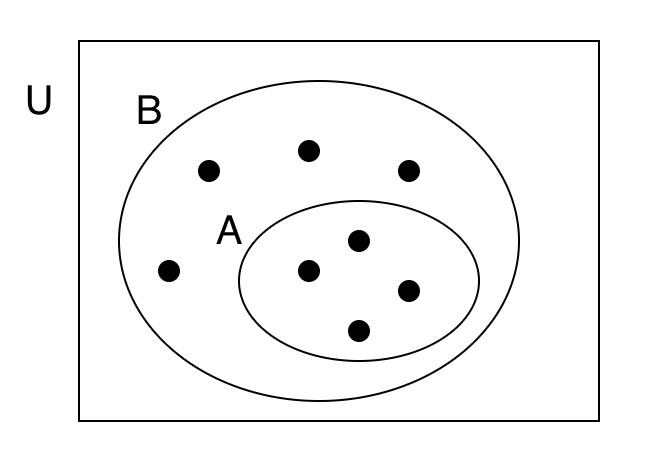
\includegraphics[width=4cm]{Eulero-venn-contenuto-uguale.png}
    \caption{Contenuto uguale}
    \label{fig:contenuto-uguale}
\end{wrapfigure}
\begin{definition}[Sottoinsieme]
	$A$ è un sottoinsieme di $B$ ($A \subseteq B$) se ogni elemento di $A$ appartiene anche a $B$. $A$ e $B$ possono essere uguali ma non è necessario. Ad esempio in figura [\ref{fig:contenuto-uguale}] $A \subseteq B$, $A \subseteq \mathbf{U}$ e $B \subseteq \mathbf{U}$ \footnote{con il simbolo "U", chiamato universo, si indicano tutti i possibili elementi che possiamo trovare in un insieme.}
\end{definition}

\begin{definition}[Sottoinsieme stretto]
	$A$ è un sottoinsieme di $B$ ($A \subset B$) se ogni elemento di $A$ appartiene anche a $B$. $A$ e $B$ non sono uguali. Ad esempio in figura [\ref{fig:contenuto-uguale}] $A \subset B$.
\end{definition}

\begin{definition}[Insiemi disgiunti]
	Due insiemi $A$ e $B$ si dicono disgiunti se non hanno elementi in comune.
	%TODO Aggiungere nel disegno un insieme C disgiunto da A e B
\end{definition}

\subsubsection{Proprietà di uguaglianza ed inclusione}
Per tutti gli insiemi A, B, C valgono le proprietà scritte in tabella \ref{tab:proprietà-uguaglianza-inclusione}.
\begin{table}[h!]
    \centering
    \setlength{\tabcolsep}{7pt}
    \renewcommand{\arraystretch}{2.5}
    \begin{tabular}{|c|c|c|}
        \hline
        \textbf{Riflessiva} & $A = A$ & $A \subseteq A$ \\
        \hline
        \textbf{Transitiva} & Se $A = B$ e $B = C \implies A = C$ & Se $A \subseteq B$ e $B \subseteq C \implies A \subseteq C$\\
        \hline
        \textbf{Simmetrica} & Se $A = B \implies B = A$ & \textit{Niente}\\
        \hline
        \textbf{Antisimmetrica} & \textit{Niente} & Se $A \subseteq B$ e $B \subseteq A \implies A = B$\\
        \hline
    \end{tabular}
    \caption{Proprietà Uguaglianza ed Inclusione}
    \label{tab:proprietà-uguaglianza-inclusione}
\end{table}

\subsubsection{Paradosso di Russell}
Sia $NV = \{X \mid X \neq \O\}$.\\
Sia $CS = \{X \mid X\ \in X\}$ l'insieme degli insiemi che appartengono a se stessi.\\
Sia $NCS = \{X \mid X \notin X\}$ l'insieme degli insiemi che non appartengono a se stessi.\\
Abbiamo un paradosso in quanto se assumiamo che $NCS \in NCS$ allora $NCS \notin NCS$, mentre se assumiamo che $NCS \notin NCS$ allora $NCS \in NCS$.

\subsection{Operazioni su insiemi}
\subsubsection{Cardinalità}
\label{sec:cardinalita}
Si rappresenta con $n$ o $\lvert A \rvert$ ed è il numero di elementi dell'insieme. Valgono le seguenti proprietà:
\begin{itemize}
	\item Se $A \subseteq B \implies \lvert A \rvert \leq \lvert B \rvert$ 
	\item Se $A = B \implies \lvert A \rvert = \lvert B \rvert$
	\item Se $A = \O \implies \vert A \rvert = 0$
\end{itemize}
\begin{note}
	Dati due insiemi $V = \{a, e, i, o ,u\}$ e $V1 = \{a, a, e, i, i, u, o, e\}$ allora $\lvert V \rvert = \lvert V1 \rvert = \lvert B \rvert$
\end{note}
\begin{example}
    Esempi cardinalità:\\
    %TODO Inserire esempi
\end{example}

\subsubsection{Unione}
\begin{figure}[h!]
	\centering
    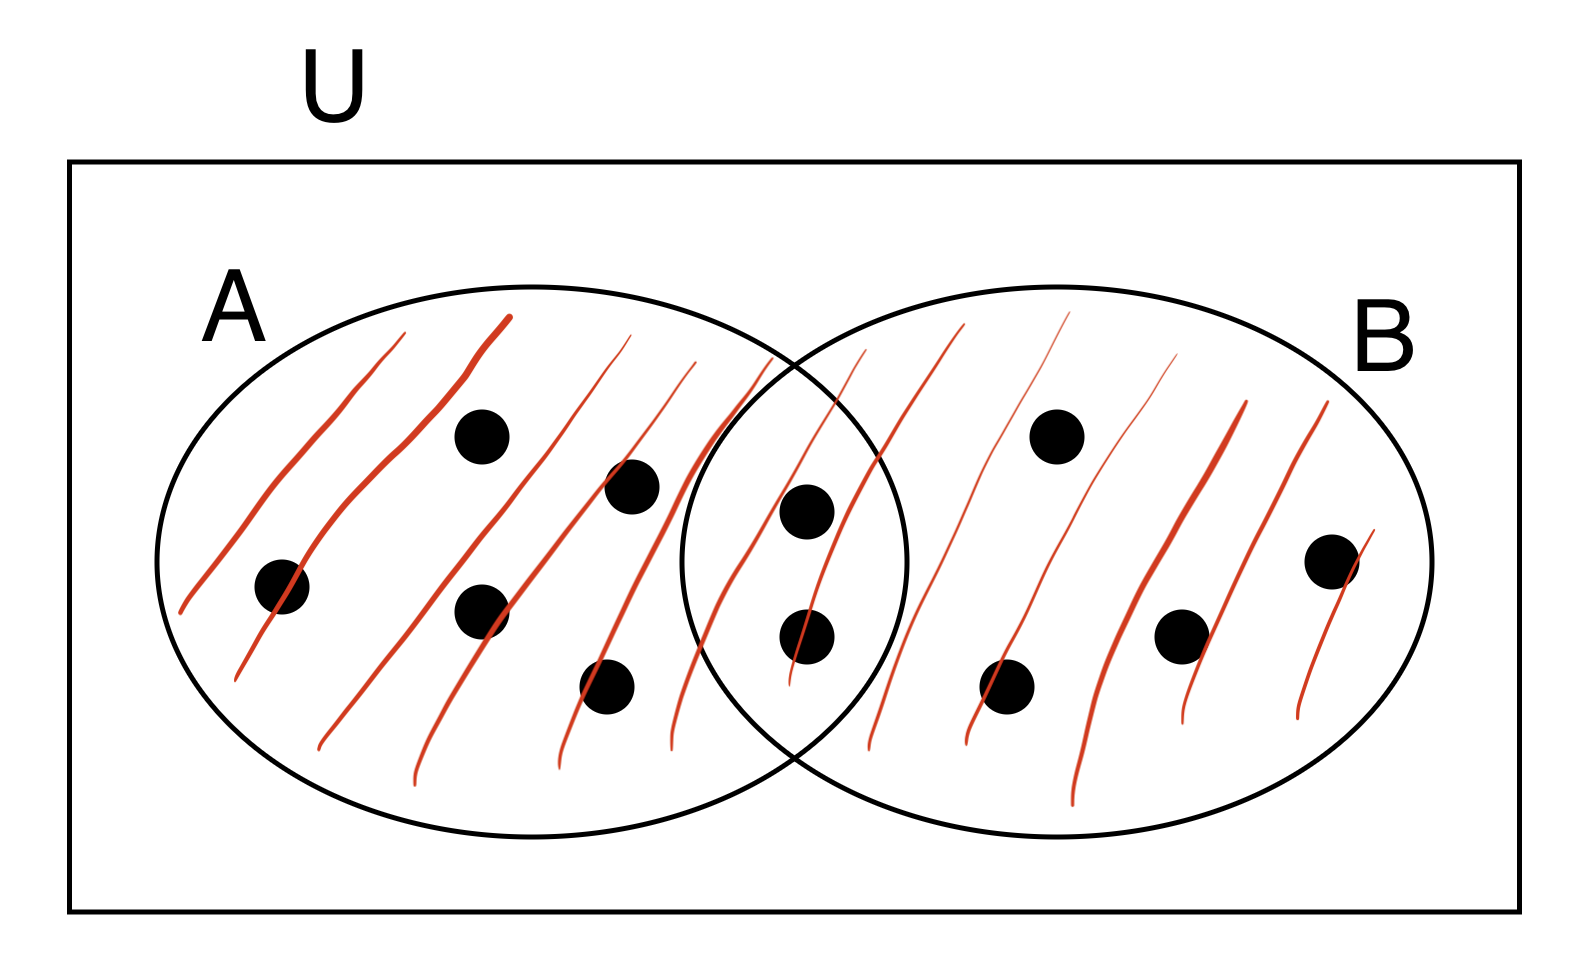
\includegraphics[width=5cm]{Unione.png}
    \caption{$A \cup B = \{x \in U \mid x \in A \vee x \in B\}$}
    \label{fig:unione}
\end{figure}

\subsubsection{Intersezione}
\begin{figure}[h!]
	\centering
	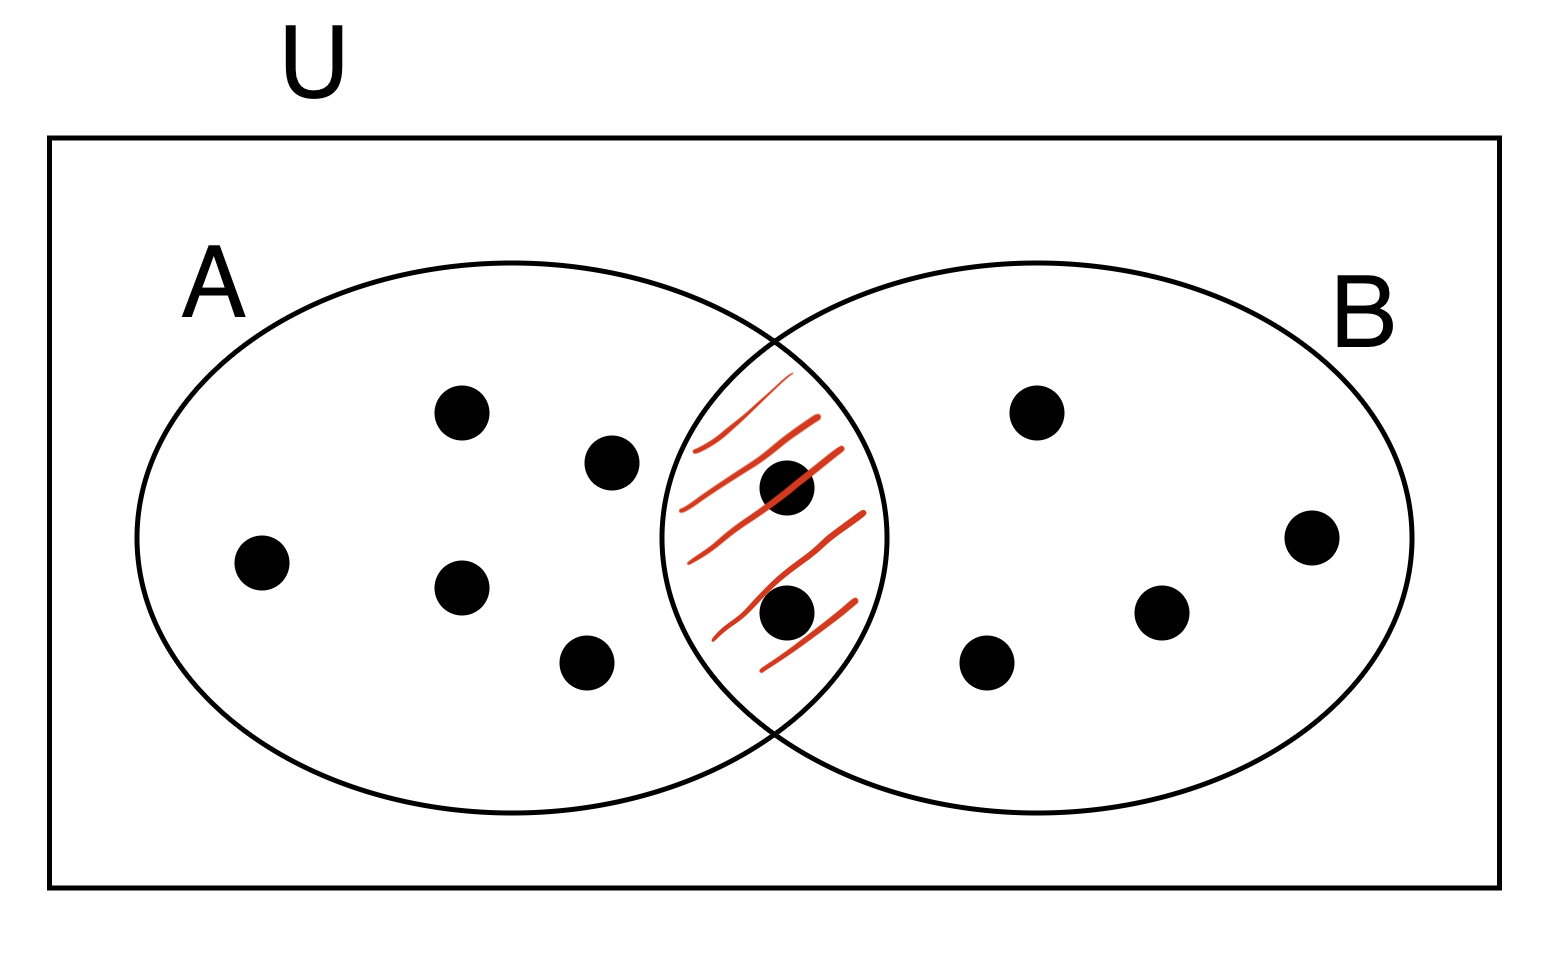
\includegraphics[width=5cm]{Intersezione.png}
	\caption{$A \cup B = \{x \in U \mid x \in A \vee x \in B\}$}
	\label{fig:intesezione}
\end{figure}

\subsubsection{Differenza}
\begin{figure}[h!]
	\centering
	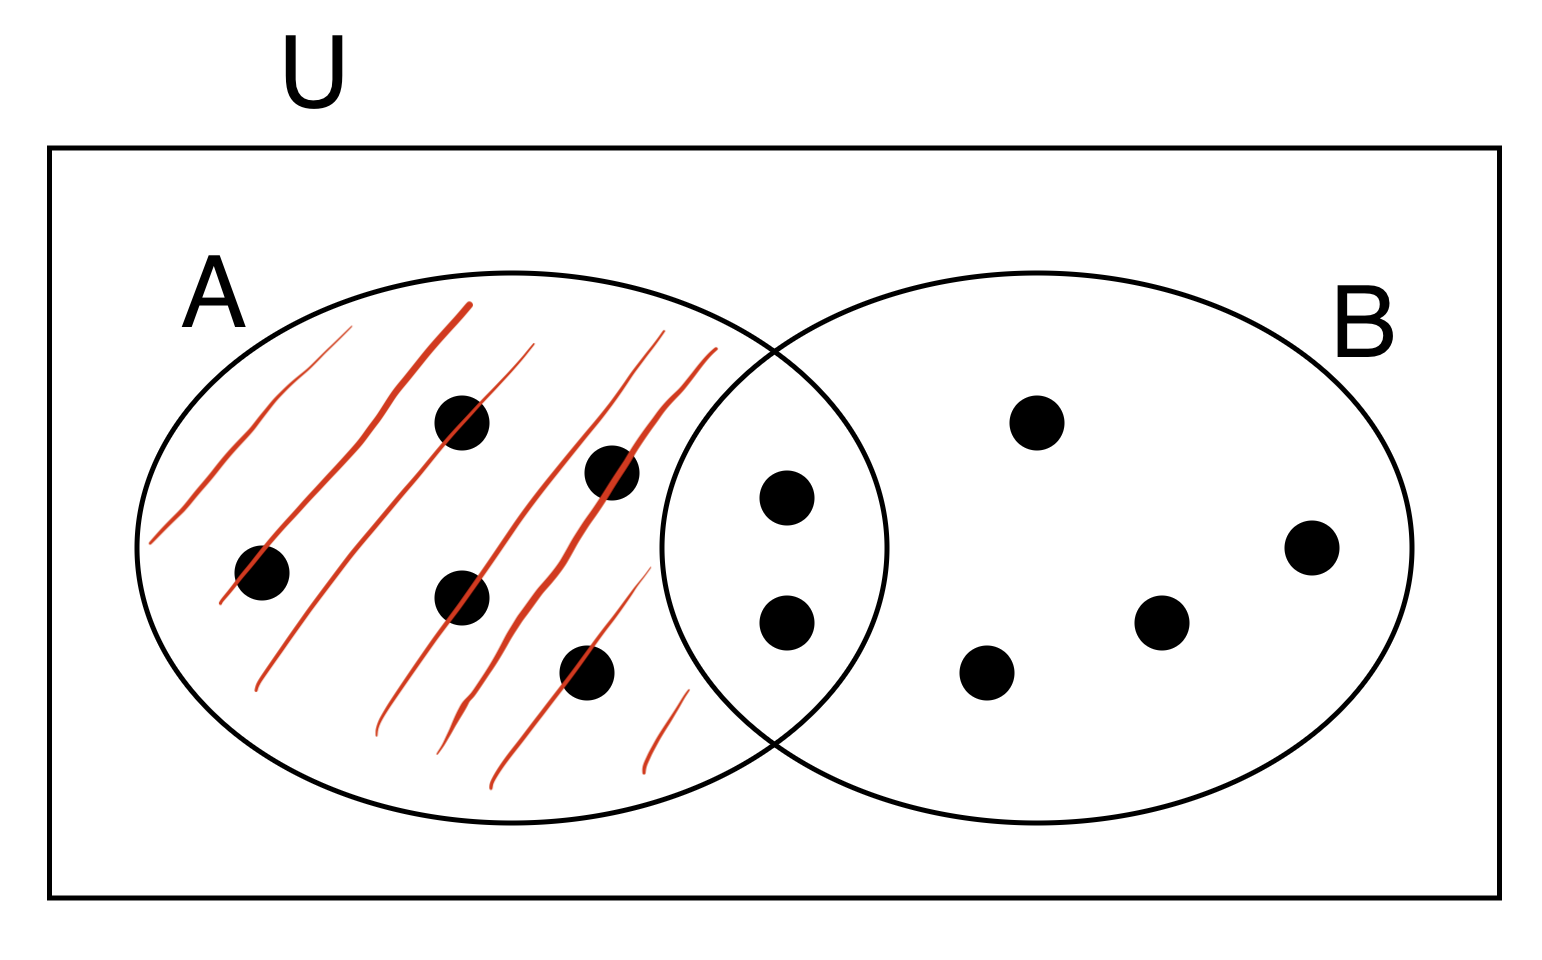
\includegraphics[width=5cm]{Differenza.png}
	\caption{$A \setminus B = \{x \in U \mid x \in A \wedge x \notin B\}$}
	\label{fig:differenza}
\end{figure}

\subsubsection{Complemento}
\begin{figure}[h!]
    \centering
    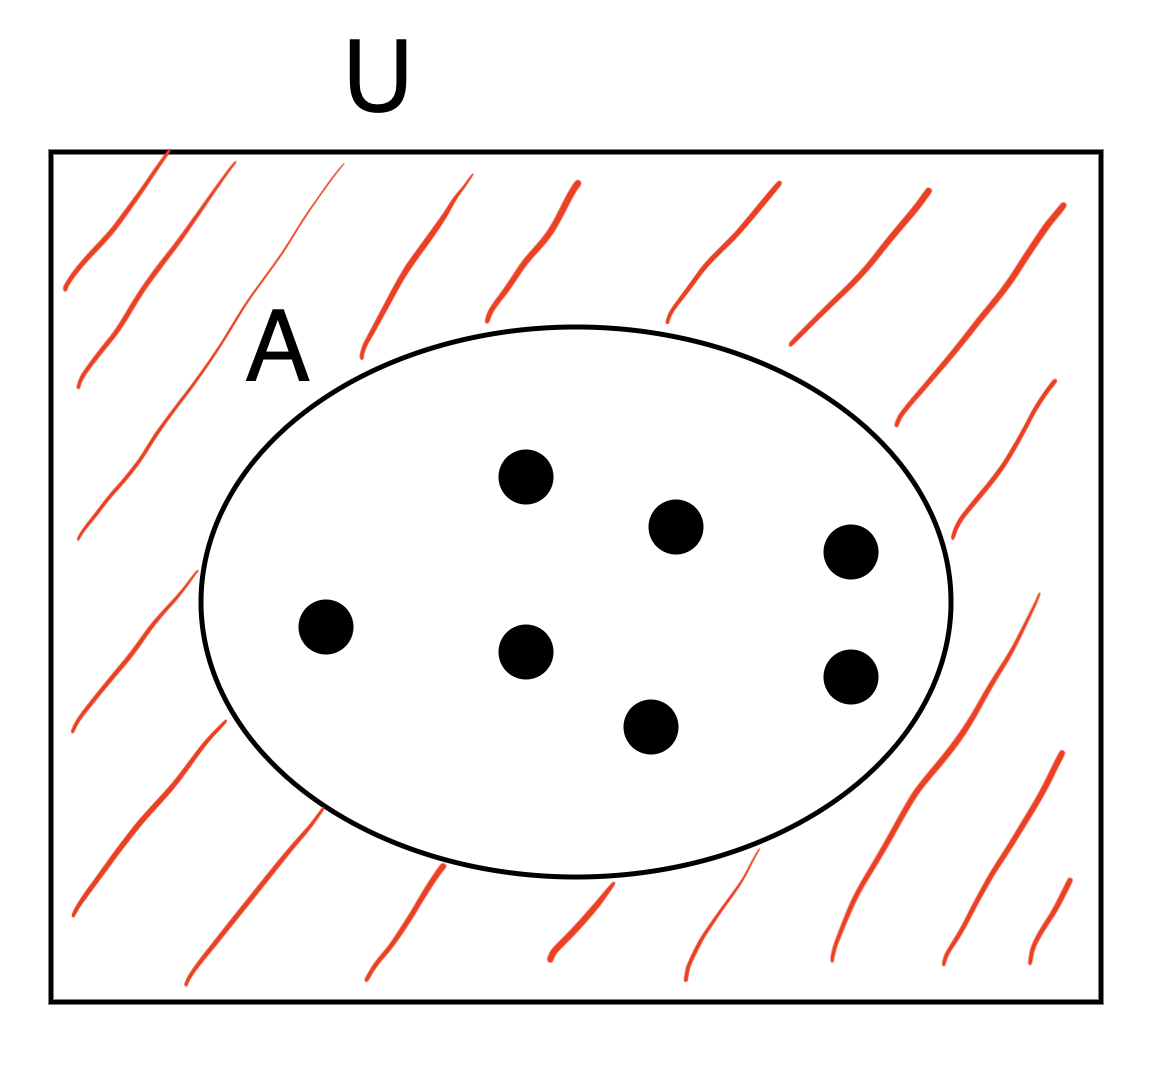
\includegraphics[width=4cm]{Complemento.png}
    \caption{$\overline{A} = \{c \in U \mid x \notin A\}$}
    \label{fig:complemento}
\end{figure}

\subsection{Tavola delle leggi}
Per tutti gli insieme A, B, C (dell'universo \textit{U}) valgono le uguaglianze nella tabella \ref{tab:leggi-insiemi}
\begin{table}[h!]
    \centering
    \setlength{\tabcolsep}{8pt}
    \renewcommand{\arraystretch}{2}
    \begin{tabular}{|c|c c|}
        \hline
        \textbf{Associazione} & $A \cup (B \cup C) = (A \cup B) \cup C$ & $A \cap (B \cap C) = (A \cap B) \cap C$ \\
        \textbf{Unita} & $A \cup \O = A$ & $A \cap U = A$ \\
        \textbf{Commutativa} & $A \cup B = B \cup A$ & $A \cap B = B \cap A$ \\
        \textbf{Indipendenza} & $A \cup A = A$ & $A \cap A = A$ \\
        \textbf{Assorbimento} & $A \cup U = U$ & $A \cap \O = \O$ \\
        \textbf{Distributiva} & $A \cup (B \cap C) = (A \cup B) \cap (A \cup C)$ & $A \cap (B \cup C) = (A \cap B) \cup (A \cap C)$ \\
        \textbf{Complemento} & $A \cup \overline{A} = U$ & $A \cap \overline{A} = \O$ \\
        \textbf{De Morgan} & $\overline{A \cup B} = \overline{A} \cap \overline{B}$ & $\overline{A \cap B} = \overline{A} \cup \overline{B}$ \\
        \textbf{Convoluzione} & $\overline{(\overline{A})} = A$ &  \\
        \textbf{Assrbimento con $\cap$ e $\cup$} & $A \cup (A \cap B) = A$ & $A \cap (A \cup B) = A$ \\
        \hline
    \end{tabular}
    \caption{Tavola delle leggi}
    \label{tab:leggi-insiemi}
\end{table}

\newpage
\subsection{Algebra di Bool}
L'algebra di bool sta alla base dell'informatica e si compone di solo 2 elementi che possono essere rappresentati in tanti modi: V - F, Vero - Falso, True - False, 1 - 0, $\O$ - U \\ \\
Su questi elementi possono essere applicate una serie di operazioni che sono: \\
\textbf{And}, \&\&, $\land$ \hspace{.3cm} \textbf{Or}, $||$, $\lor$ \hspace{.3cm} \textbf{Not}, $\sim$, $\lnot$
\textbf{Implicazione:}\footnote{La parte a sinistra della freccia si chiama \textbf{premessa}, la parte a destra invece \textbf{conseguenza}} $A \Longrightarrow B$, se $A$ allora $B$ \\
\textbf{Conseguenza:} $A \Longleftarrow B$, $A$ se $B$ \\ 
\textbf{Doppia implicazione:} $A \iff B$, $A$ se e solo se $B$

\begin{table}[h!]
    \centering
    \setlength{\tabcolsep}{10pt}
    \renewcommand{\arraystretch}{1.5}
    \begin{tabular}{c|c|c|c|c|c|c|c}
        A & B & $A \land B$ & $A \lor B$ & $\lnot A$ & $A \Longrightarrow B$ & $A \Longleftarrow B$ & $A \iff B$\\
        \hline
        \O & \O & \O & \O & U & U & U & U\\
        \O & U & \O & U & U & U & \O & \O\\ 
        U & \O & \O & U & \O & \O & U & \O\\ 
        U & U & U & U & \O & U & U & U
    \end{tabular}
    \caption{Operazioni con algebra booleana}
\end{table}
\begin{note}
Se nella tabella andiamo a sostituire lo \O \: con 0 e U con 1 o con qualsiasi altro valore corrispondente nell'algebra di boole il risultato resta invariato.
\end{note}

\subsection{Dimostrazioni}
Una \textbf{legge} è \textbf{valida} se vale per tutte le scelte dell'insieme che prendiamo in considerazione. Una \textbf{dimostrazione} indica la validità di una legge. Un \textbf{controesempio} mostra che la legge non è valida per almeno un caso (appunto il controesempio).
Ci sono 3 tecniche di dimostrazione: \textbf{grafica} (diagramma di Eulero-Venn), \textbf{discorsiva} e tramite \textbf{sostituzione}.

\subsubsection{Grafica}
\begin{example}
    Dimostriamo la legge distributiva mediamente i diagrammi di Eulero-Venn.
    \begin{equation}
    	A \cup (B \cap C) = (A \cup B) \cap (A \cup C)
    \end{equation}
	%TODO inserire il titolo per la serie di diagrammi: prima il lato sinistro della dimostrazione e poi il lato destro
    \begin{figure}[h!]
        \begin{subfigure}{.3\textwidth}
            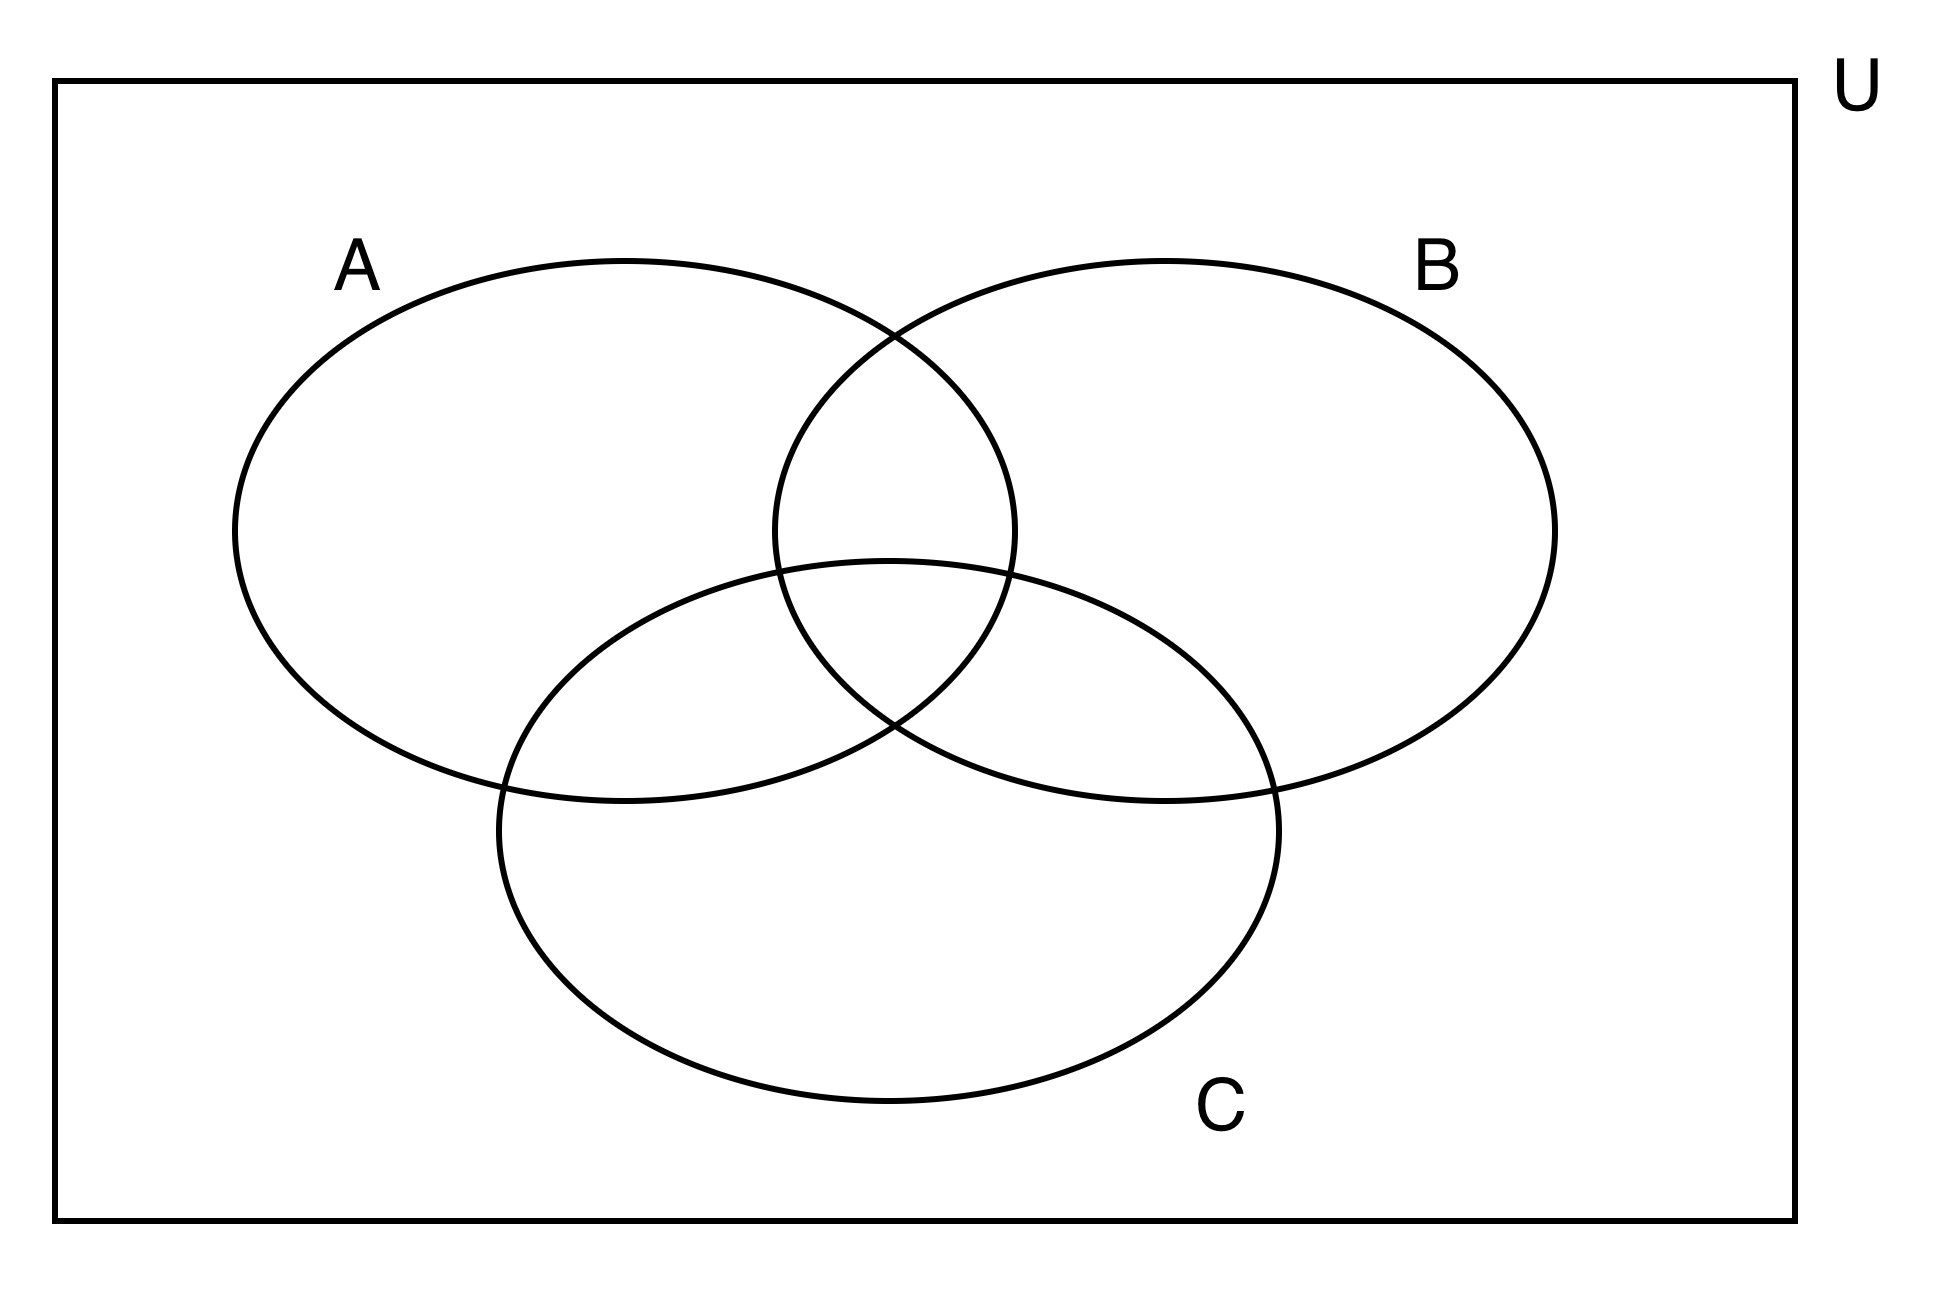
\includegraphics[width=4cm]{Dimostrazione-distibutiva-eulero-venn-1.png}
            \caption{Insiemi di partenza}
            \label{fig:Dimostrazione-distibutiva-eulero-venn-1}
        \end{subfigure}
        \hfill
        \begin{subfigure}{.3\textwidth}
            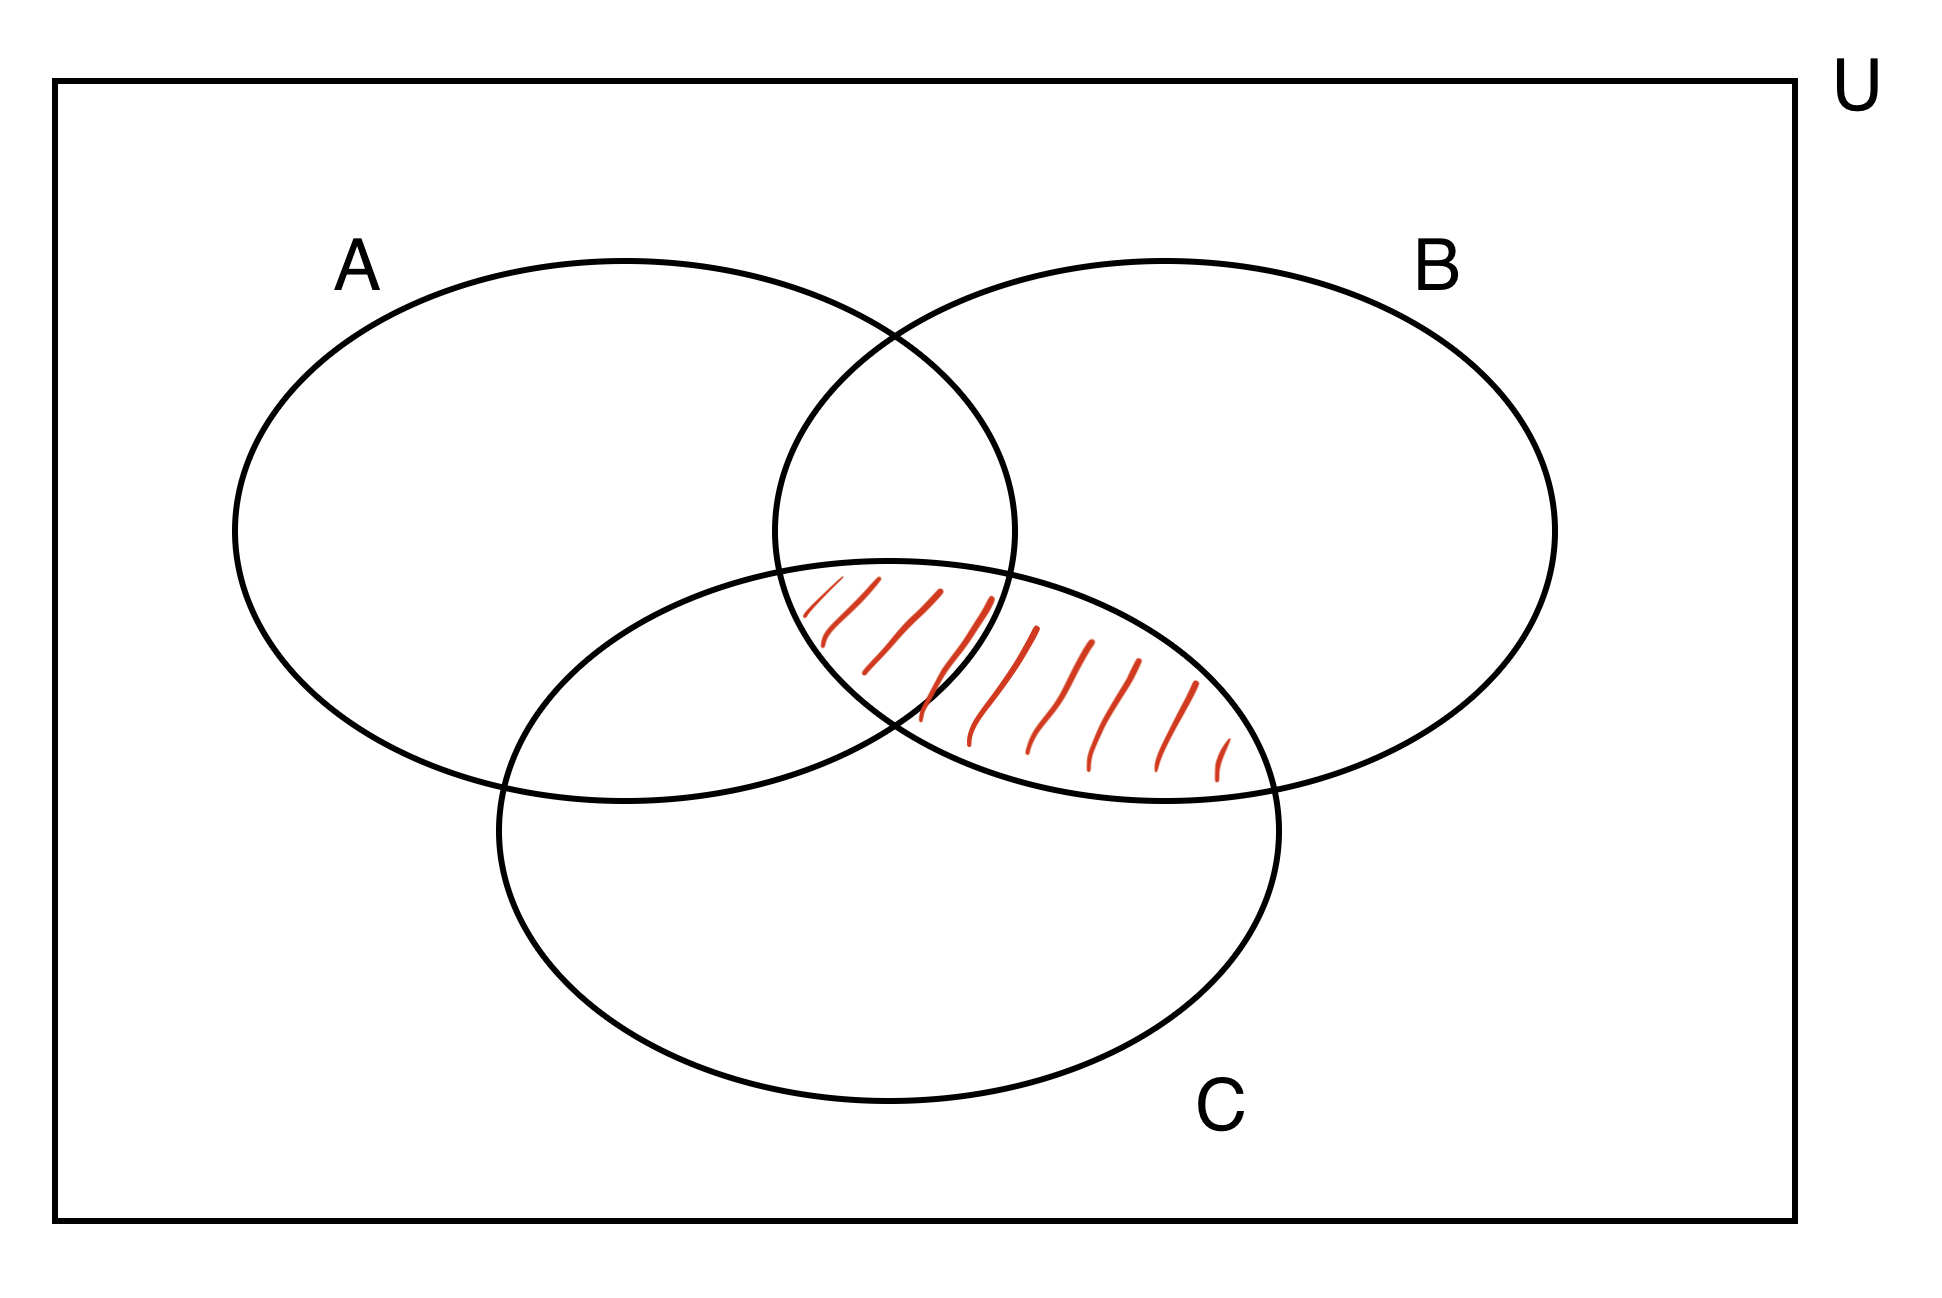
\includegraphics[width=4cm]{Dimostrazione-distibutiva-eulero-venn-2.png}
            \caption{Step 1 - $B \cap C$}
            \label{fig:Dimostrazione-distibutiva-eulero-venn-2}
        \end{subfigure}
        \hfill
        \begin{subfigure}{.3\textwidth}
            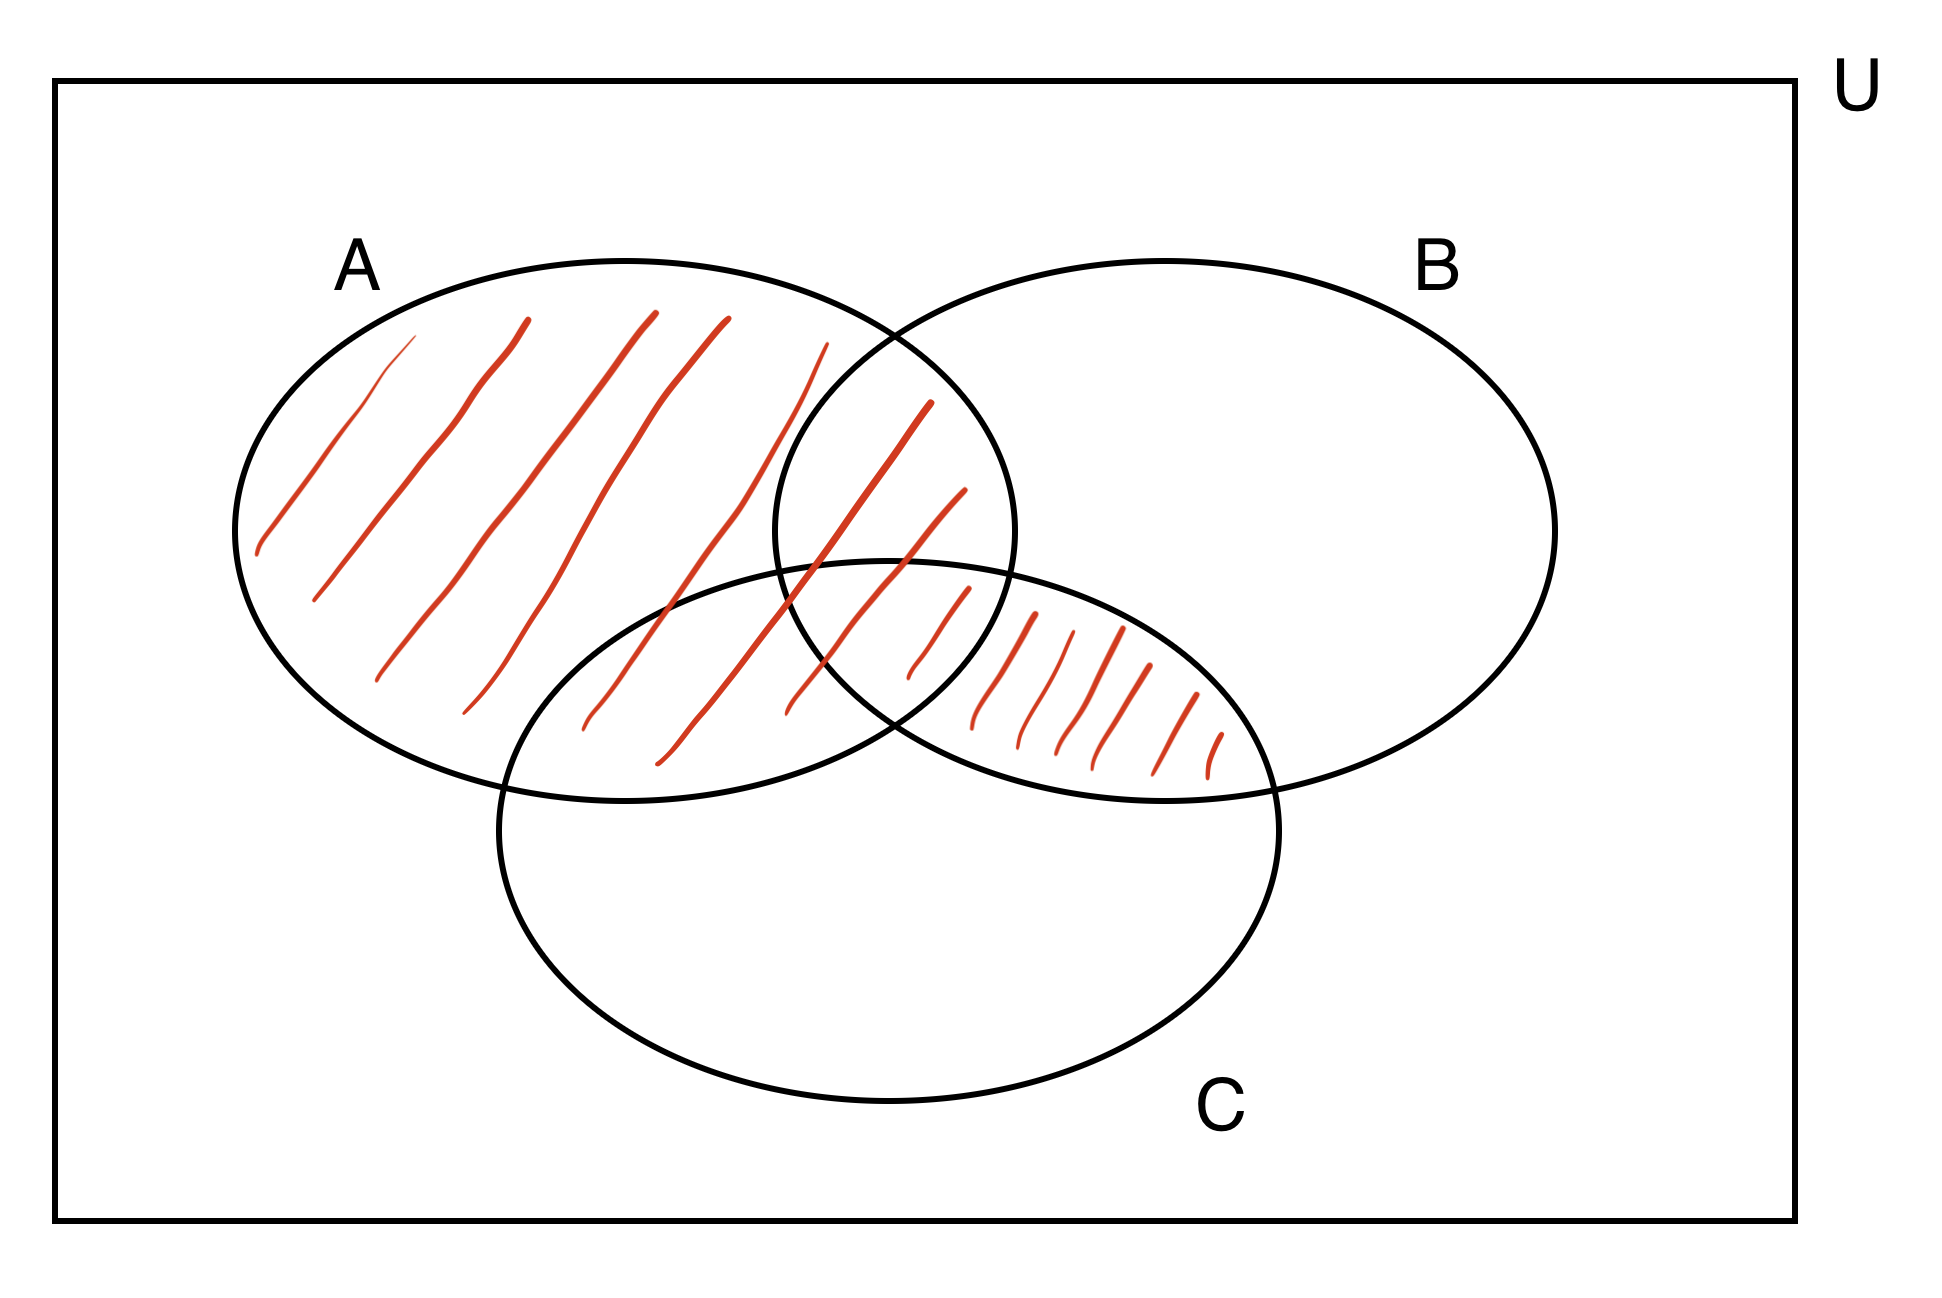
\includegraphics[width=4cm]{Dimostrazione-distibutiva-eulero-venn-3.png}
            \caption{Step 2 - $A \cup (B \cap C)$}
            \label{fig:Dimostrazione-distibutiva-eulero-venn-3}
        \end{subfigure}
    \end{figure}
    \begin{figure}[h!]
        \begin{subfigure}{.3\textwidth}
            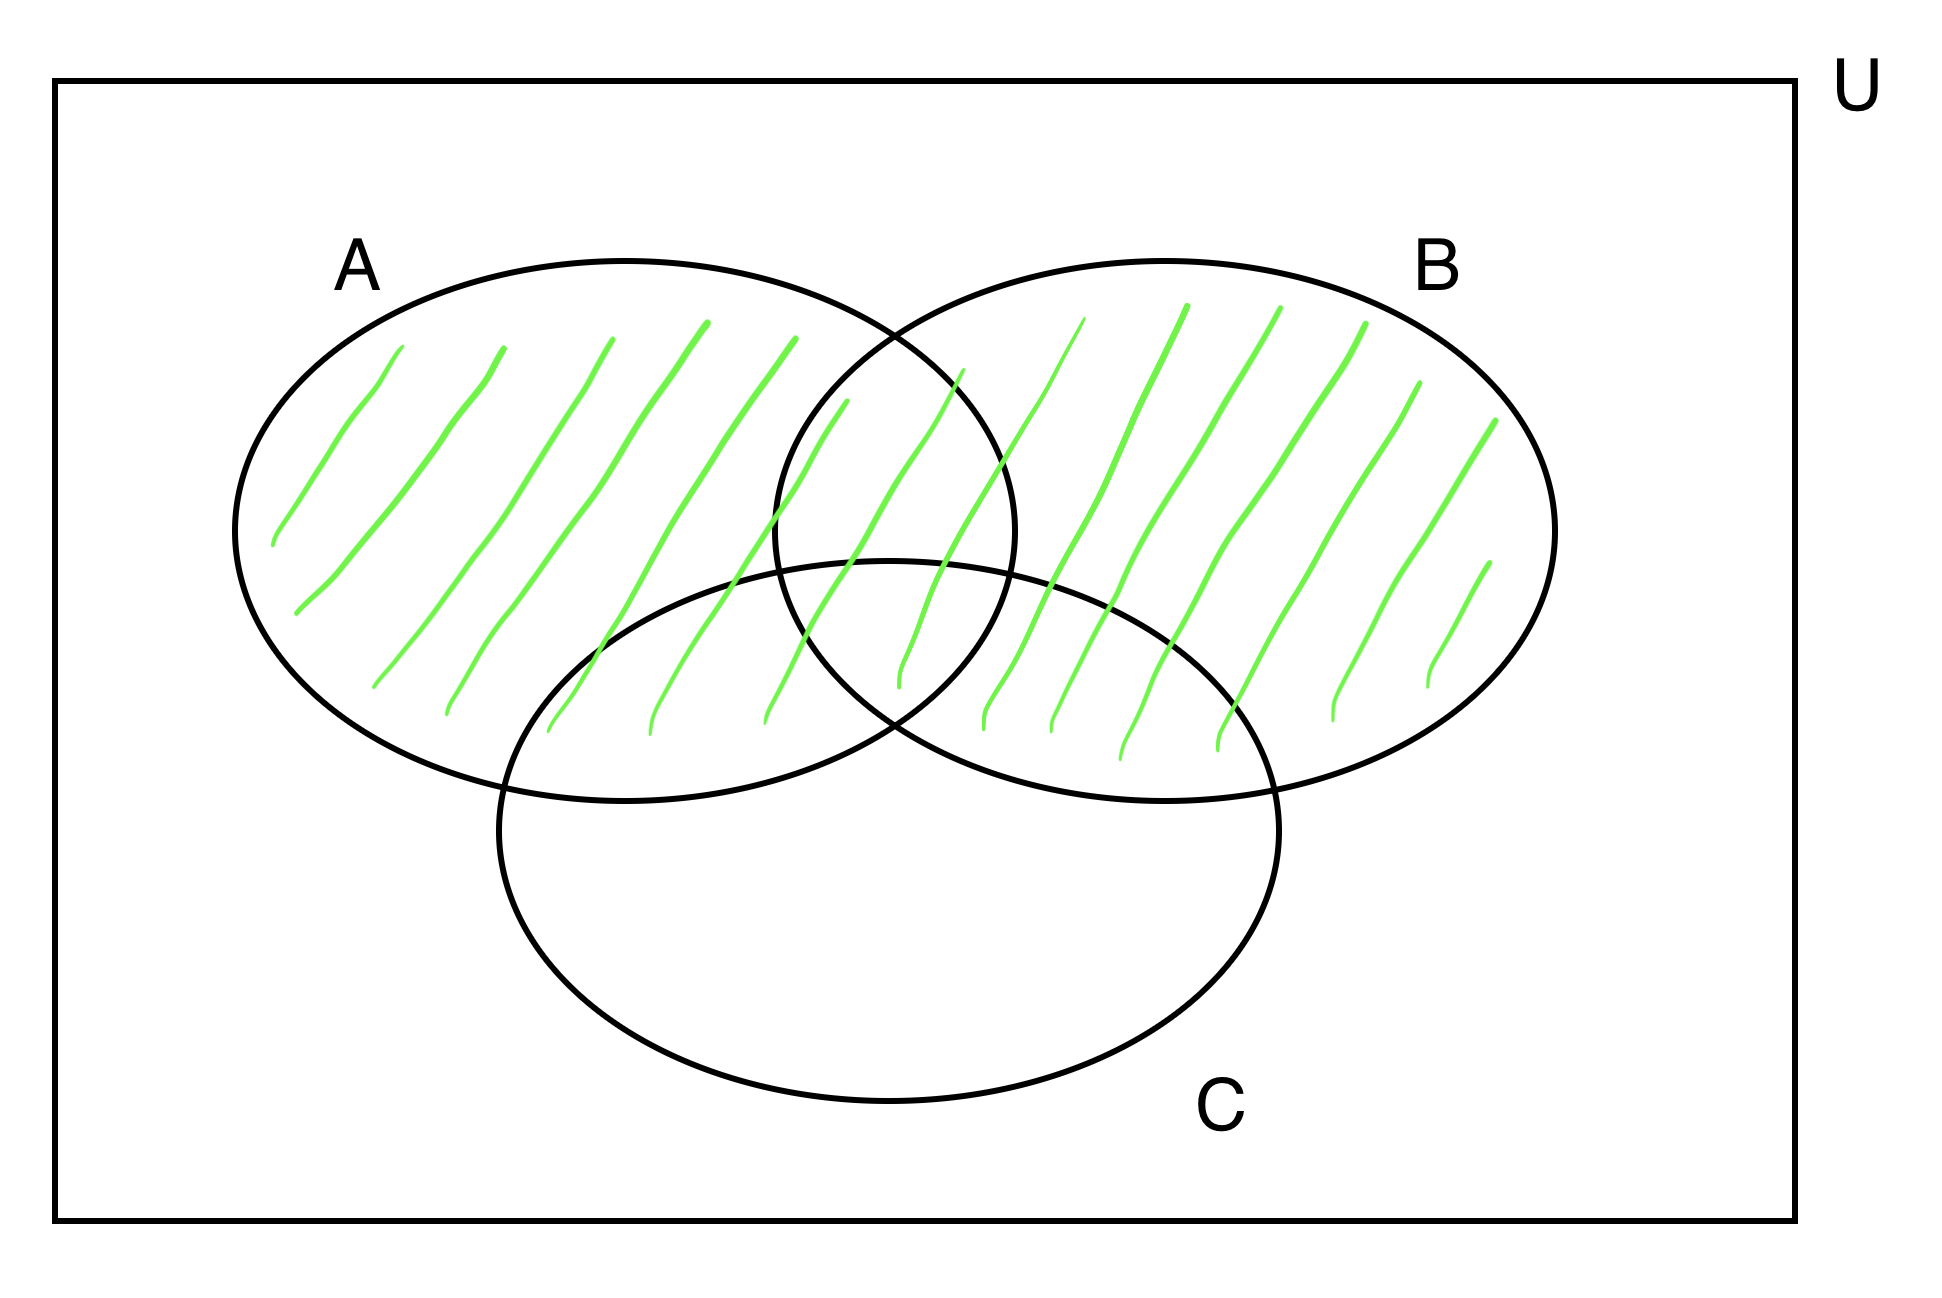
\includegraphics[width=4cm]{Dimostrazione-distibutiva-eulero-venn-4.png}
            \caption{Step 3 - $A \cup B$}
            \label{fig:Dimostrazione-distibutiva-eulero-venn-4}
        \end{subfigure}
        \hfill
        \begin{subfigure}{.3\textwidth}
            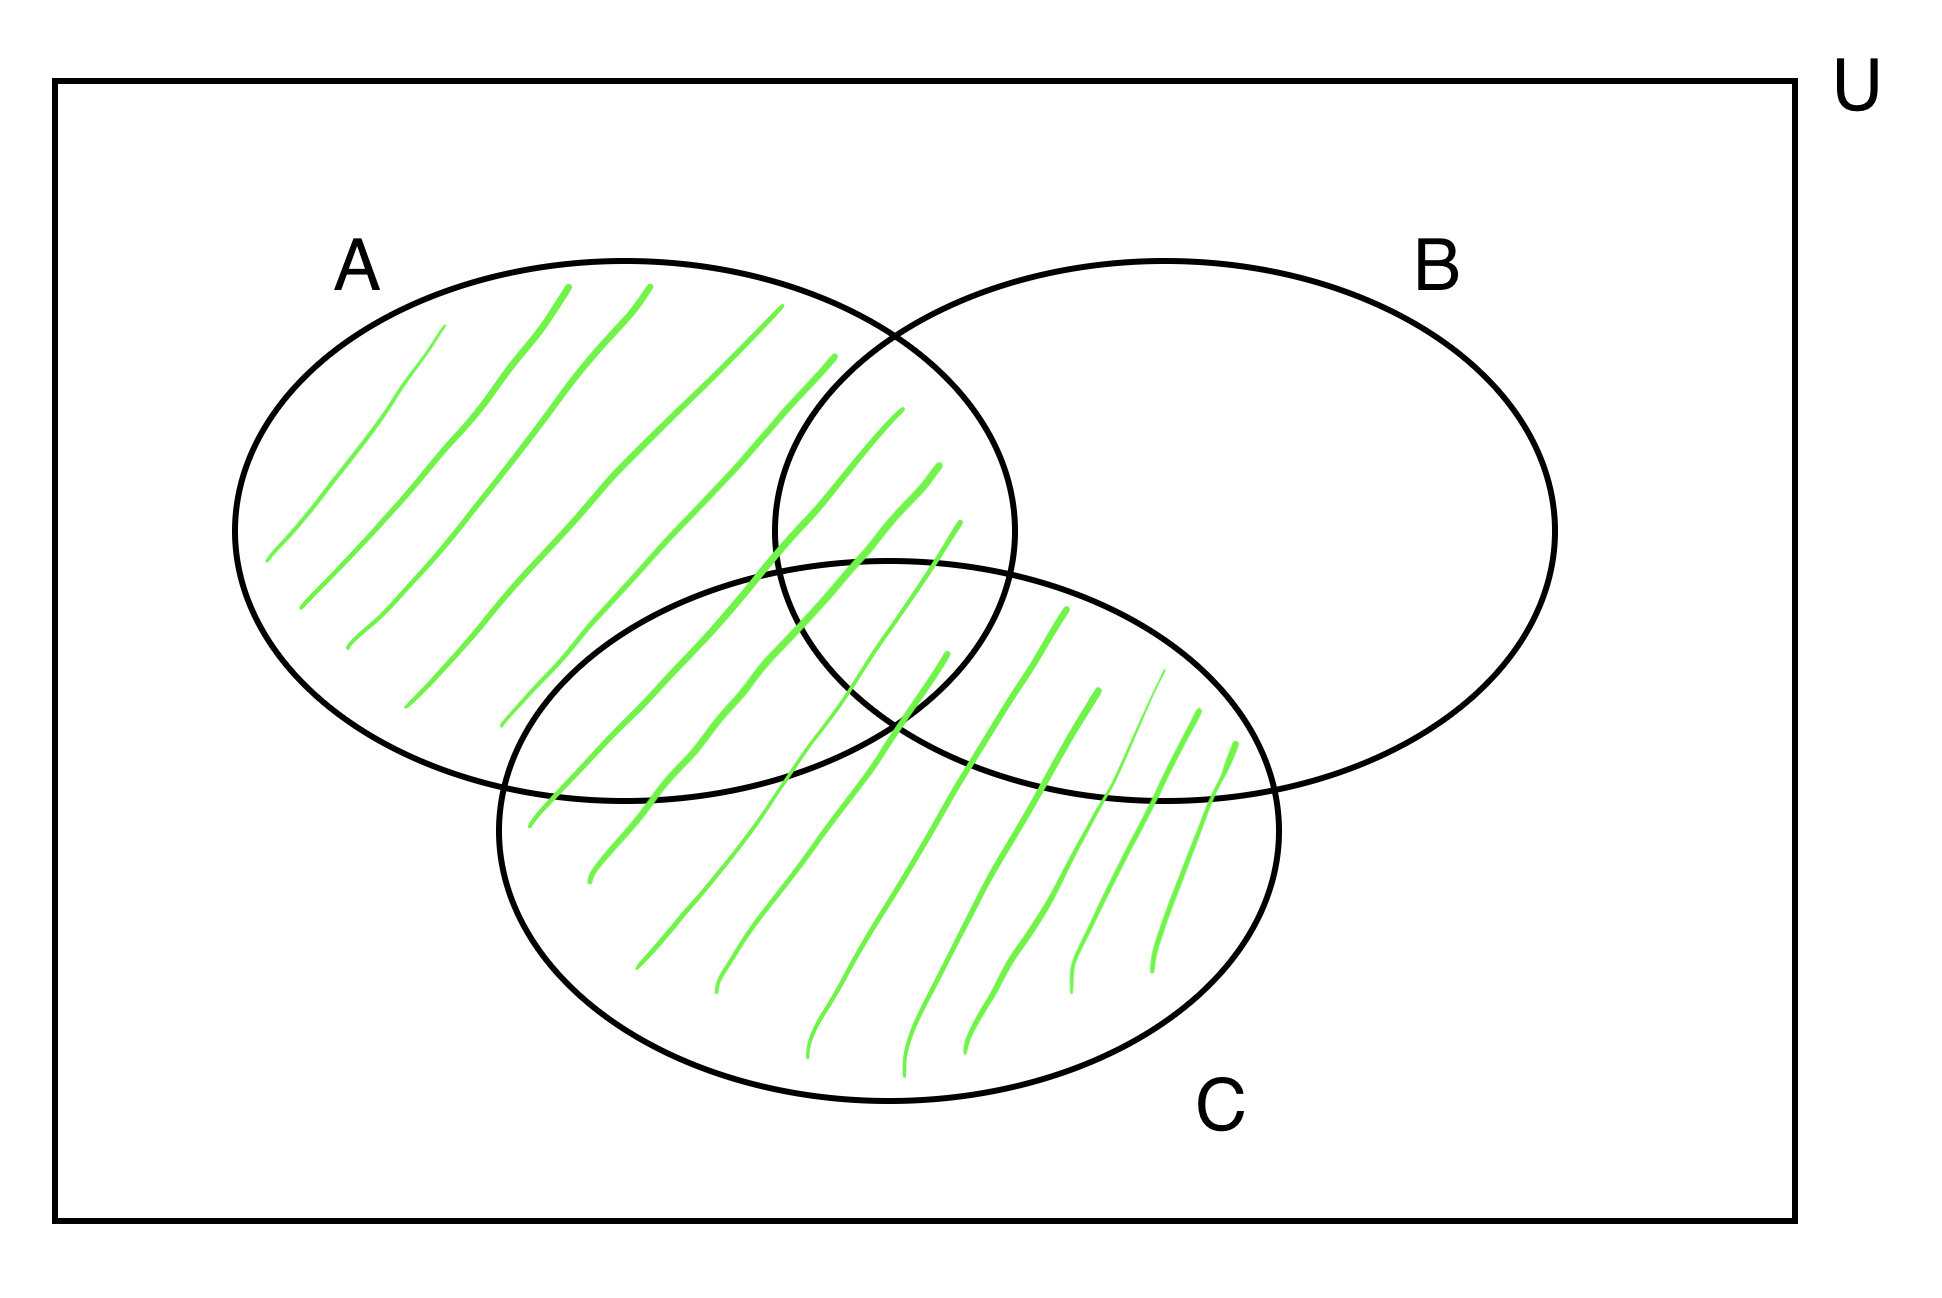
\includegraphics[width=4cm]{Dimostrazione-distibutiva-eulero-venn-5.png}
            \caption{Step 4 - $A \cup C$}
            \label{fig:Dimostrazione-distibutiva-eulero-venn-5}
        \end{subfigure}
        \hfill
        \begin{subfigure}{.3\textwidth}
            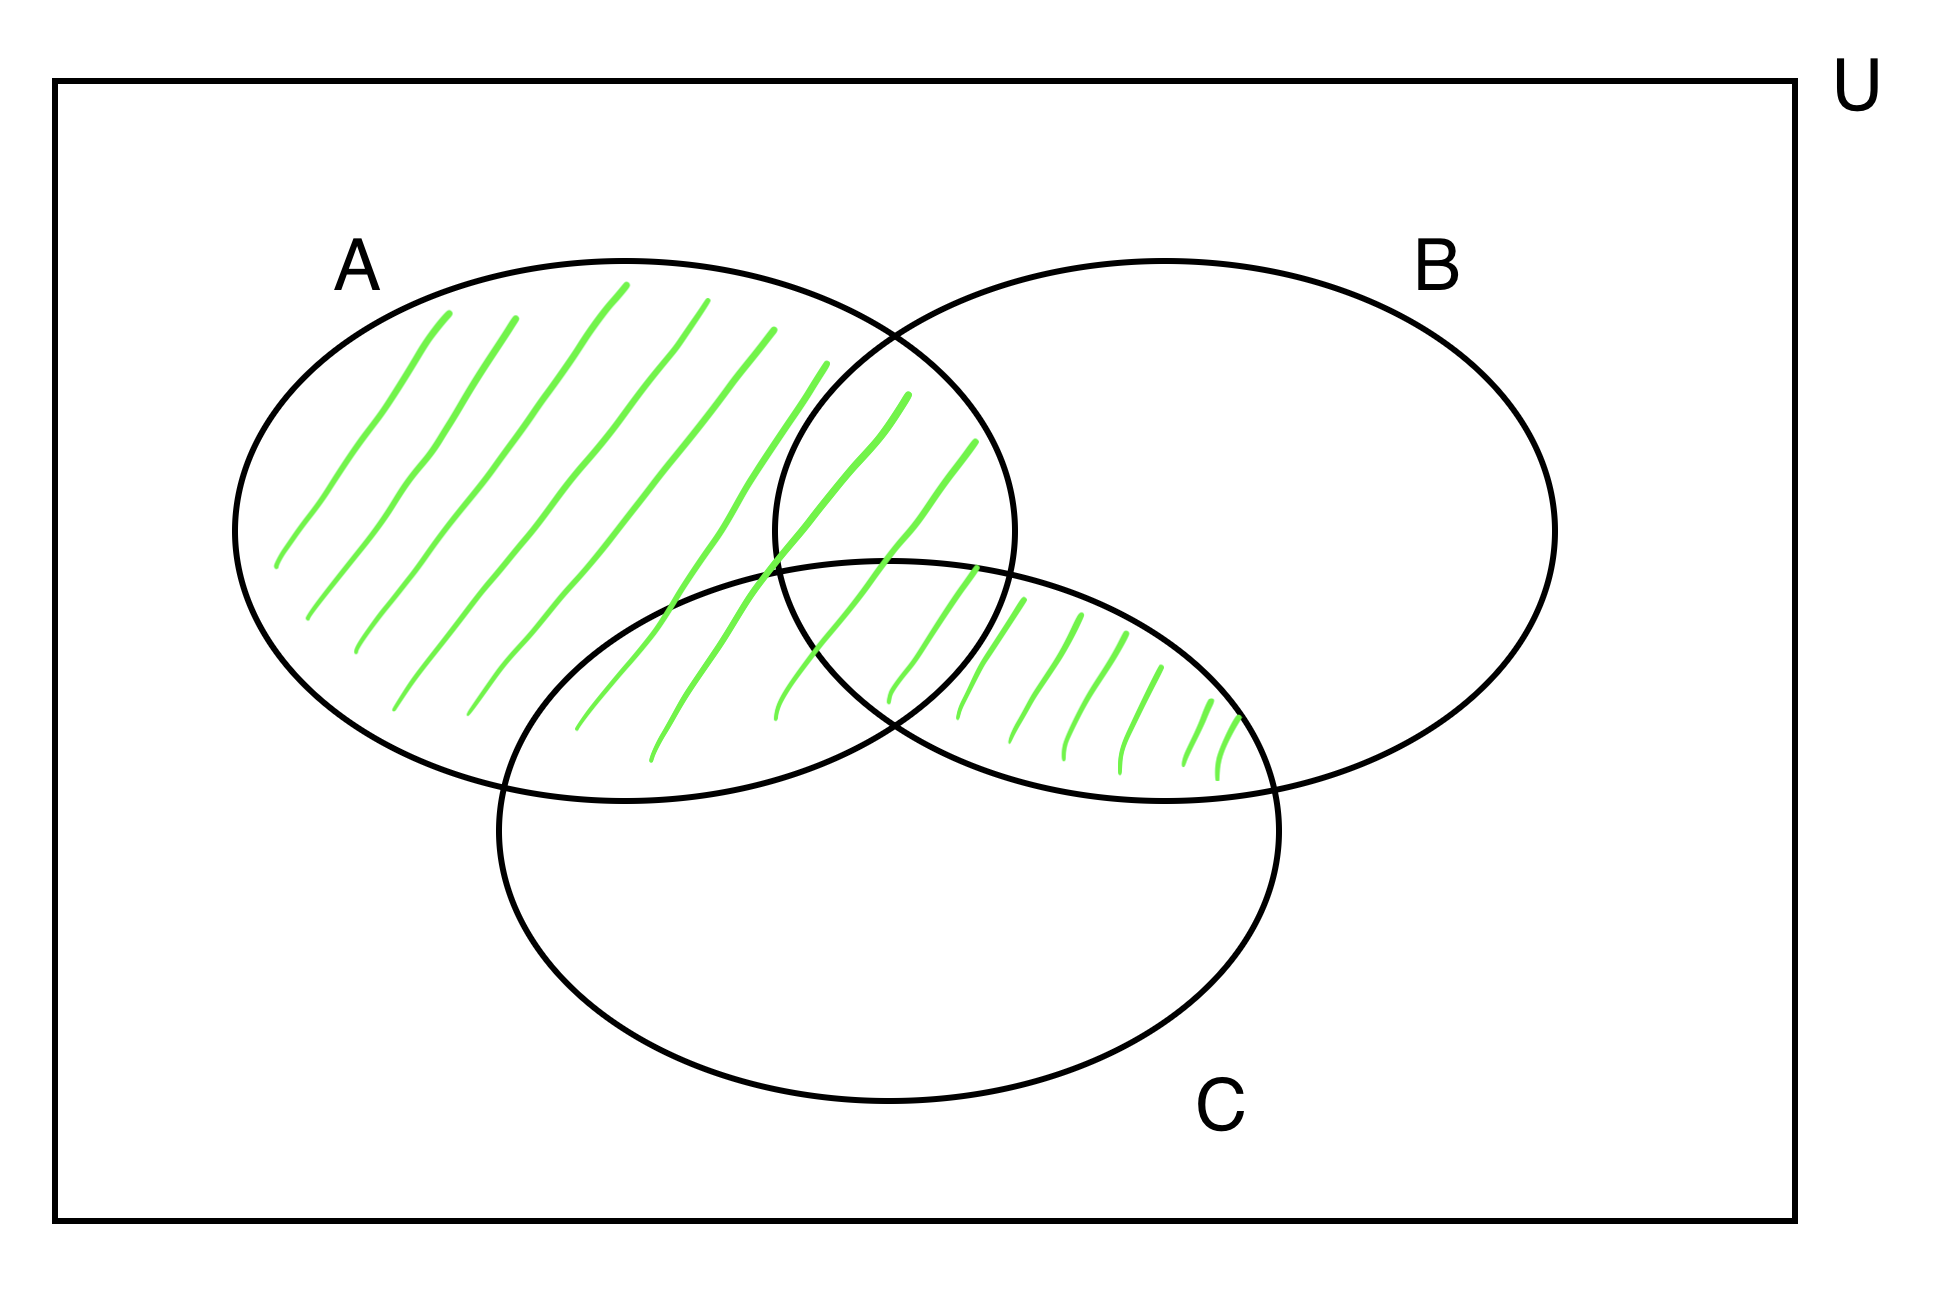
\includegraphics[width=4cm]{Dimostrazione-distibutiva-eulero-venn-6.png}
            \caption{Step 5 - $(A \cup B) \cap (A \cup C)$}
            \label{fig:Dimostrazione-distibutiva-eulero-venn-6}
        \end{subfigure}
    \end{figure}
    \\ Possiamo vedere come lo step 2 (\ref{fig:Dimostrazione-distibutiva-eulero-venn-2}), che rappresenta ciò che dovrebbe essere $A \cup (B \cap C)$ con i diagrammi di eulero-venn, e lo step 5 (\ref{fig:Dimostrazione-distibutiva-eulero-venn-5}), cioè $(A \cup B) \cap (A \cup C)$, siano uguali e quindi possiamo dire che la proprietà e dimostrata.  
\end{example}


\subsubsection{Sostituzione}
Questo tipo di dimostrazione si basa sull'utilizzare leggi preesistenti per dimostrare un'affermazione, scomponendo tale affermazione in modo che si possa ricorrere ad un legge fondamentale.
\begin{example}
    $(A \cup B) \cup C = A \cup (C \cup B)$
    \begin{enumerate}
        \item \textbf{Commutativa}: $(A \cup B) \cup C = A \cup (\mathbf{B \cup C})$
    \end{enumerate}
    L'ipotesi è vera per la proprietà \emph{associativa}.
\end{example}
\begin{example}
    $A \cup (\overline{A} \cap B)$
    \begin{enumerate}
        \item Usando la \textbf{Distributiva} possiamo dividere la prima parte: $(A \cup \overline{A}) \cap (A \cup B) = (A \cup B)$
        \item Usando la proprietà del \textbf{Complemento} $A \cup \overline{A}$ diventa U quindi perché un insieme unito con la sua negazione torna sempre l'universo: $U \cap (A \cup B) = (A \cup B) $
        \item Per la proprietà dell'\textbf{Unità} un insieme A unito con l'universo U è uguale a l'insieme stesso quindi: $A \cup B = A \cup B$
    \end{enumerate}
    L'ipotesi è così verificata.
\end{example}
 
\subsubsection{Discorsiva}
Esempio di dimostrazione della proprietà distributiva:
\begin{equation}
	A \cup (B \cap C) = (A \cup B) \cap (A \cup C)
\end{equation}
Teniamo conto che: $X = Y \iff (X \subseteq Y) \land (Y \subseteq X)$.\\
Andiamo a questo punto a sostituire X con la prima parte della proprietà distributiva, $A \cup (B \cap C)$ e Y con la seconda $(A \cup B) \cap (A \cup C)$. 
Applicando la considerazione scritta sopra otteniamo due condizione che devono entrambi essere vere per far si che la condizione di uguaglianza iniziale $A \cup (B \cap C) = (A \cup B) \cap (A \cup C)$ sia vera e quindi la proprietà sia verificata. Queste due condizioni sono:
\begin{itemize}
    \item $A \cup (B \cap C) \subseteq (A \cup B) \cap (A \cup C)$ - \underline{Dimostrazione 1°}
    \item $(A \cup B) \cap (A \cup C) \subseteq A \cup (B \cap C)$ - \underline{Dimostrazione 2°}
\end{itemize}
\textbf{Dimostrazione 1°}: $A \cup (B \cap C) \subseteq (A \cup B) \cap (A \cup C)$\\
\textit{Ricordiamo che un insieme $W \subseteq Z$ per ogni $x \in W$ e $z \in Z$.}\\
Sostituendo la W con la prima parte, $A \cup (B \cap C)$, e la Z con la seconda, $(A \cup B) \cap (A \cup C)$ possiamo scrivere che $y \in A \cup (B \cap C)$. Per la definizione di unione possiamo distinguere in 2 casi.
\begin{center}
    (1a) $y \in A$ \hspace{.5cm}  (1b) $y \in (B \cap C)$ \\
\end{center}
Da qui il nostro obbiettivo è far valere per entrambi i casi che $y \in (A \cup B) \cap (A \cup C)$.
\begin{itemize}
    \item \textbf{Caso 1a:} $y \in A$
    \begin{enumerate}
        \item Per questo caso possiamo vedere come, per la definizione di unione, aggiungendo qualsiasi cosa all'insieme A l'appartenenza di y rimarrà invariata. Quindi $y \in A \cup B$, $y \in A \cup C$.
        \item Da qui per la definizione di intersezione\footnote{\textit{($y \in W \cap Z, \iff y \in W \: e \: y \in Z$)}} $y \in (A \cup B) \cap (A \cup C)$. Caso dimostrato. $\blacksquare$
    \end{enumerate}
    \item \textbf{Caso 1b:} $y \in (B \cap C)$
    \begin{enumerate}
        \item Siccome $x \in B \cap C$, per definizione di intersezione si ha che $x \in B$ e che $x \in C$.
        \item Dato che $x \in B$, a sua volta ha che $x \in A \cup B$.
        \item Analogamente, dato che $x \in C$, per definizione di unione si ha che $x \in A \cup C$.
        \item Ma allora, visto che x appartiene a entrambi questi insiemi deve appartenere anche alla
        loro intersezione, ovvero $y \in (A \cup B) \cap (A \cup C)$. Caso dimostrato. $\blacksquare$
    \end{enumerate}
\end{itemize}
\textbf{Dimostrazione 2°}: $(A \cup B) \cap (A \cup C) \subseteq A \cup (B \cap C)$ \\
Come per la dimostrazione 1° andiamo a prendere qualsiasi elemento $y \in (A \cup B) \cap (A \cup C)$.\\
Da qui per la definizione di intersezione $y \in (A \cup B)$ e $y \in (A \cup B)$ che ci permette di conseguenza di distinguere 4 casi:
\begin{center}
    (1) $y \in A$ e $y \in A$ \hfill
    (2) $y \in A$ e $y \in B$ \hfill
    (3) $y \in C$ e $y \in A$ \hfill
    (4) $y \in B$ e $y \in C$
\end{center}
Però possiamo racchiudere le prime 3 con $y \in A$ e l'ultima come $y \notin A$. Quindi abbiamo due possibilità disgiunti fra loro.
\begin{center}
    (2a) $y \in A$ \hspace{.5cm}  (2b) $y \notin A$ \\
\end{center}
In entrambi i casi bisogna arrivare a dimostrare che $y \in A \cup (B \cap C)$.
\begin{itemize}
    \item \textbf{Caso 2a:} $y \in A$
    \begin{enumerate}
        \item Essendo che $y \in A$ allora per definizione di unione $y \in A \cup (B \cap C)$. Caso dimostrato. $\blacksquare$
    \end{enumerate}
    \item \textbf{Caso 2b:} $y \notin A$
    \begin{enumerate}
        \item Dato che $y \in A \cup B$ ma $y \notin A$, allora necessariamente $y \in B$.
        \item Analogamente, data che $y \in A \cup C$ ma $y \notin A$, allora $y \in C$.
        \item Visto che y apparitene sia a B che a C deve per forza appartenere alla loro intersezione, quindi $y \in (B \cap C)$.
        \item A questo punto per definizione di unione $y \in A \cup (B \cap C)$. Caso dimostrato. $\blacksquare$
    \end{enumerate}
\end{itemize}
Non avendo nessun' altro caso da dimostrare abbiamo concluso la dimostrazione. $\blacksquare$

\subsection{Prodotto Cartesiano}
Prendendo 2 insiemi A, B il loro prodotto cartesiano si definisce come:
\begin{center}
    $A \times B = \{(a, b) \mid a \in A, b \in B\}$
\end{center}
\begin{note}
	In un prodotto cartesiano $\lvert A \times B \rvert = \lvert A \rvert * \lvert B \rvert$ e $A \times \O = \O$
\end{note}
\begin{example}
    Esempio prodotto cartesiano:\\
    $A = \{501234, 501227, 678980\}$ N. matricola \hspace{1cm}
    $B = \{18, 19, 20, ..., 30L\}$ Voti \\
    $A \: X \: B = \{(501234, 18), (501234, 19), ..., (678980, 30L)\}$\\ \\
    I sottoinsiemi che si vanno a creare con il prodotto cartesiano si indicano con le parentesi tonde "($\ldots$)" e possono essere di due tipi:
    \begin{itemize}
        \item \textbf{Coppia Ordinata:} si tiene conto dell'ordinamento degli elementi. E.g. $(a, b) \neq (b, a)$.
        \item \textbf{Coppia Non Ordinata:} non si tiene conto dell'ordinamento degli elementi. E.g. $(a, b) = (b, a)$.
	\end{itemize}
\end{example}

\subsection{Insiemi di insiemi}
\begin{definition}
Un insieme di insiemi è quando uno o più elementi di un insieme è a sua volta un insieme.
\end{definition}
\begin{note}
	Preso $A = \{\{a\}, \{a, b\}, \{a, b, c\}\}$, si nota che $a \notin A$ mentre $\{a\} \in A$.
\end{note}
\begin{note}
	Sapendo che $\O = \{\}$ possiamo dedurre che $\lvert \{\{\}\}\rvert = 1$.
\end{note}
\begin{example}
Esempi insiemi di insiemi:
    \begin{itemize}
        \item $X = \{a, \{a, b, c\}, \{a, \{b\}\}, \{\{c\},d\}\}$
        \item $N = \{\{\}, \{\{\}\}, \{\{\{\}\}\}, \{\{\{\{\}\}\}\}, ...\} = \mathbb{N}$
    \end{itemize}
\end{example}

\subsubsection{Insieme delle parti}
\begin{definition}
Dato un insieme $A$, l'insieme delle parti di $A$ si indica come $P(A)$ e si definisce come tutti i possibili sottoinsiemi di $A$.
\begin{equation}
	P(A) = \{x \subseteq A\}
\end{equation}
\begin{note}
	La \hyperref[sec:cardinalita]{\textbf{cardinalità}} nell'insieme delle parti si calcola come: $P(A) = 2^{|A|}$
\end{note}
\end{definition}
\begin{example}
    Con $A = \{a, b, c\}$, $P(A) = \{\O, \{a\}, \{b\}, \{c\}, \{a, b\}, \{a, c\}, \{c, b\}, \{a, b, c\}\}$
\end{example}

\section{Relazioni}
\begin{definition}[Relazione]
	\label{def:relazione}
	Prendiamo in considerazione un prodotto cartesiano con due insieme $A, B$ che sia $A \times B = \{(a,b) \: | \: a \in A, b \in B\} = $ U (Universo). 
	\\
	Una relazione è $R \subseteq U$ dove, come scritto sopra, $U = A \times B$.
	\\
	In una relazione A è detto \textbf{insieme di partenza} e B è detto \textbf{insieme di arrivo}.
\end{definition}

%TODO Magari si può rimuovere questo hspace
\hspace{-15pt}
In sintesi possiamo definire una relazione come un sottoinsieme del prodotto cartesiano fra due insiemi.
\\
L'insieme $rel(A,B)$ è l'inseme di tutte le possibili relazioni fra $A$ e $B$.
\begin{example}
    Esempio relazione.\\
    Prendiamo due insiemi e facciamo il prodotto cartesiano.
    \begin{itemize}
    	\item Insieme degli \textbf{studenti} $S = \{luca, mario, angela, gino, maria\}$
    	\item Insieme dei \textbf{corsi} $C = \{PA, LAB, FI, AN\}$
    \end{itemize}
    Il prodotto cartesiano fra $S$ e $C$ è uguale a tutte le possibile coppie ordinate che si possono formare fra i due insieme, quindi:
    \begin{equation}
    	S \times C = \{(luca, PA), (luca, LAB), ..., (marica, AN)\}
    \end{equation}
    In questo caso possiamo creare una relazione del prodotto cartesiano andando appunto a prendere un sottoinsieme di $A \times B$ e stabilendo una regola o condizione per scegliere quali coppie ordinate vogliamo, ad esempio $R \subseteq A \times B$ è una relazione che specifica quali esami sono stati sostenuti dai vari studenti.
\end{example}

\subsection{Identità}
Quando l'insieme di partenza e quello di arrivo coincidono, si ottengono alcuni casi particolari di \hyperref[def:relazione]{relazioni}. Un esempio è il seguente:
\begin{example}
	Sia $\mathbb{U}$ l'insieme di tutti gli esseri umani, e consideriamo le seguenti relazioni di parentela:
	\begin{itemize}
		\item $Madre = {(x, y) \in \mathbb{U} \times \mathbb{U} \implies x \text{ madre di } y}$
		\item $Padre = {(x, y) \in \mathbb{U} \times \mathbb{U} \implies x \text{ padre di } y}$
		\item $Figlia = {(x, y) \in \mathbb{U} \times \mathbb{U} \implies x \text{ figlio di } y}$
		\item $Figlio = {(x, y) \in \mathbb{U} \times \mathbb{U} \implies x \text{ figlia di } y}$
	\end{itemize}
\end{example}
\begin{example}[Identità]
Preso un insieme A, l'identità su A è una relazione con se stessa, e si scrive $Id_A \subseteq$ A X A. Si può quindi vedere come nell'identità di un insieme ogni elementi è identico a se stesso. Inoltre l'identità di un insieme si definisce come:
\end{example}
\vspace{-10pt}
\begin{equation}
    Id_A = \{(a,a) \mid a \in A\}
\end{equation}
\vspace{-20pt}
\subsection{Composizione}
\begin{definition}[Composizione]
Siano $R: A \rightarrow B$ e $S: B \rightarrow C$. La \textbf{composizione} di R con S è la relazione $R;S: A \rightarrow C$ così definita:
\end{definition}
%TODO Aggiungere esempio fatto a lezione con sorella e zia (vedi slide)
%TODO Aggiungere immagini
\begin{equation}
    R;S = \{(x, z) \in A \times C \mid \exists b \in B . (x, y) \in R \land (y,z) \in S\}\footnote{Il simbolo "." indica \emph{tale che}. Ad esempio $\exists x.P$ indica che esiste un x per cui vale la proprietà P.}
\end{equation}

\begin{note}
	L'insieme di arrivo di R deve essere uguale all'insieme di partenza di S per effettuare l'operazione di composizione.
\end{note}

%TODO Fare l'esempio basandosi su padre/madre ma con nonni (vedi dispensa)
\begin{example}
\end{example}

\subsection{Relazione opposta}
\begin{definition}[Relazione opposta]
Sia $R:A\rightarrow B$ una relazione. La \textbf{relazione opposta} di $R$ è la relazione $R^{op}:B\rightarrow A$ definita come: 
\begin{equation}
	R^{op} = \{(y, x) \in B \times A \mid (x, y) \in R\}
\end{equation}
\end{definition}
%TODO OSS: non posso fare Rop;Sop in quanto l'insieme di partenza di Sop non è l'insieme di arrivo di Rop. posso però fare Sop;Rop. Inserisci grafico preso da slide

\begin{example}
    A = $\{$pagine web$\}$ \hspace{.5cm} B = $\{$parole del vocabolario$\}$ \hspace{.5cm} $R \subseteq$ A X B\\
    Si associa ciascuna pagina web con le parole in essa contenuta:
    \begin{itemize}
        \item $(x, y) \in \mathbb{R}$ dice che nella pagina web "x" è contenuta la parola "y".
        \item $R^{op}$ ($(y, x) \in \mathbb{R}$) dice per ogni parola "y" quali sono le pagine web che le contengono.
    \end{itemize}
\end{example}

\subsection{Leggi}
Come per gli insiemi, anche per le relazioni esistono delle leggi che regolano il comportamento delle varie operazioni. \\ \\
Per tutti gli insiemi A, B, C, D e per tutte le relazioni $R \subseteq A \times B$, $S \subseteq B \times C$, $T \subseteq C \times D$, valgono le leggi scritte nelle tabelle \ref{tab:leggi-composizione}, \ref{tab:leggi-relazioni-opposte}, \ref{tab:leggi-distributività}, una volta preso $A \times B$ come universo.
\begin{table}[h!]
    \setlength{\tabcolsep}{8pt}
    \renewcommand{\arraystretch}{2}
    \centering
    \begin{tabular}{|c|c|}
    \hline
        \textbf{Associatività} & (R;S);T = R;(S;T) \\
        \textbf{Unità} & $Id_A$;R = R;$Id_B$ = R \\
        \textbf{Assorbimento} & $\O$;S = S;$\O$ = $\O$ \\ \hline
    \end{tabular}
    \caption{Leggi composizione}
    \label{tab:leggi-composizione}
\end{table}
\begin{table}[h!]
    \vspace{-10pt}
    \centering
    \setlength{\tabcolsep}{8pt}
    \renewcommand{\arraystretch}{2}
    \begin{tabular}{|c|c|}
        \hline
        \textbf{Convoluzione} & $(R^{op})^{op} = R$ \\
        \textbf{Opposto-identità} & $(Id)^{op} = Id$ \\
        \textbf{Opposto-complemento} & $($A X B$)^{op}$ = (B X A) \\
        \textbf{Opposto-vuoto} & $(\O)^{op} = \O$ \\ \hline
    \end{tabular}
    \caption{Leggi relazioni opposte}
    \label{tab:leggi-relazioni-opposte}
\end{table}
\begin{table}[h!]
    \vspace{-10pt}
    \centering
    \setlength{\tabcolsep}{8pt}
    \renewcommand{\arraystretch}{2}
    \begin{tabular}{|c|c|c|}
        \hline
        \textbf{Distributività composizione} & R;(S $\cup$ T) = (R;S) $\cup$ (R;T) & (S $\cup$ T); R = (S;R) $\cup$ (T;R) \\
        \textbf{Distributività opposto} & $(R \cup S)^{op}$ = $S^{op} \cup R^{op}$ & $(R \cap S)^{op}$ = $S^{op} \cap R^{op}$ \\
        \textbf{Distributività opposto su negazione} & $(\overline{R})^{op} = (\overline{R^{op}})$ & \\
        \textbf{Distributività opposto su composizione} & $($R;S$)^{op}$ = $S^{op}$;$R^{op}$ & \\ \hline
    \end{tabular}
    \caption{Leggi distributività}
    \label{tab:leggi-distributività}
\end{table}
\\
%TODO Sistemare la spiegazione delle leggi citando la definizione e usando maybe le subsections
\textbf{Spiegazione Associatività:}\\
R;S $\subseteq$ A X C, facendo la composizione con T la prima parte dell'uguaglianza (R;S);T $\subseteq$ A X D. A sua volta, analizzando la seconda parte dell'uguaglianza, S;T $\subseteq$ B X D che poi se andiamo a comporre con R risulta che R;(S;T) $\subseteq$ A X D. Possiamo così vedere che l'uguaglianza è verificata. Per la dimostrazione discorsiva completa vedere in seguito. \\ \\
\textbf{Spiegazione Unità:}\\
Essendo che $Id_A = A \times A$ e $Id_B = B \times B$ vediamo che la prima parte dell'uguaglianza $Id_A;R = A \times B$ e la seconda è $R;Id_B = A \times B$, quindi la prima uguaglianza è verificata. La seconda uguaglianza si verifica in automatico visto che $A \times B = R$.

%TODO OSS: Dimostrare che data R:A->B allora R;(BxC)=AxB è falso (vedi slide)

\subsubsection{Dimostrazione proprietà associativa}
\begin{demostration}
    Facciamo una dimostrazione discorsiva della proprietà associativa in tabella \ref{tab:leggi-composizione}.\\
    Proprietà associativa: (R;S);T = R;(S;T) \hspace{.3cm} Con: $R \subseteq$ A X B, \: \: $S \subseteq$ B X C, \: \: $T \subseteq$ C X D.\\ \\
    \textit{Innanzitutto ricordiamo la proprietà per cui dati 2 insiemi X, Y $X = Y \Longleftrightarrow X \subseteq Y \land Y \subseteq X$.} \\
    Utilizziamo la proprietà sopra scritto andando a sostituire alla X "(R;S);T" e alla Y "R;(S;T)", troviamo così due condizioni che, per l'operatore logico $\land$, devono essere vere entrambe per far valere l'uguaglianza:
    \begin{itemize}
        \item (R;S);T $\subseteq$ R;(S;T) - \underline{Dimostrazione 1°}.
        \item R;(S;T) $\subseteq$ (R;S);T - \underline{Dimostrazione 2°}.
    \end{itemize}
        \underline{Dimostrazione 1°}: (R;S);T $\subseteq$ R;(S;T) \\ 
        \textit{Come prima cosa ricordiamo che un insieme $W \subseteq Z \: \: \forall \: w \in W \land z \in Z$.} \\
        Sostituendo "(R;S);T" a W e "R;(S;T)" a Z troviamo che, per fare in modo che la condizione che un insieme sia sottoinsieme di un altro $\forall \: (a,d) \in$ (R;S);T $ \land \: (a,d) \in$ R;(S;T). \footnote{Ricordati che (R;S);T ha al suo interno coppie (a,d) $\subseteq$ A X D per le operazioni di composizione}\\ \\
        Noi dobbiamo dimostrare che $\forall \: (a,d) \in$ R;(S;T) sia vera:\\
        Prendiamo come prima cosa una generica coppia di valori (a,d) $\in$ (R;S);T. Perché esista questa coppia deve esistere per forza un valore "c" che faccia da ponte fra "(R;S)" e "T" (ricordiamo che R;S $\subseteq$ A X C e T $\subseteq$ C X D). Possiamo scrivere quindi (Colore \textbf{nero} nella rappresentazione [\ref{fig:rappresentazioni-dim-associtiva}]):
        \begin{equation}
            (a,d) \in (R;S);T \Longrightarrow \: \exists \: c \in C \: \bullet (a,c) \in R;S \land (c,d) \in T \text{ (Nel disegno freccia NERA)}
            \label{eq:dim1-associtiva-1}
        \end{equation}
        Ora nella forma scritta sopra [\ref{eq:dim1-associtiva-1}] abbiamo una parte (a,c) $\in$ R;S che deve essere "scomposta" in maniera specifica per verificare che tutta la composizione di partenza sia vera, infatti deve esistere un valore b che colleghi l'insieme R ed S nell'operazione di composizione R;S (ricordiamolo che R $\subseteq$ A X B e R $\subseteq$ B X S). Possiamo scrivere quindi (Colore \textbf{blu} nella rappresentazione [\ref{fig:rappresentazioni-dim-associtiva}]):
        \begin{equation}
            (a,d) \in (R;S);T \Longrightarrow \: \exists \: b \in B, \: c \in C \: \bullet (a,b) \in R \land (b,c) \in S \land (c,d) \in T \text{ (Nel disegno freccia BLU)}
            \label{eq:dim1-associtiva-2}
        \end{equation}
        Ora per arrivare alla forma che dobbiamo dimostrare, R;(S;T), l'ultima forma [\ref{eq:dim1-associtiva-2}] è troppo estesa, infatti la parte $(b,c) \in S \land (c,d) \in T$ deve essere racchiusa per arrivare alla forma S;T. Quindi andiamo a scrivere che (Colore \textbf{rosso} nella rappresentazione [\ref{fig:rappresentazioni-dim-associtiva}]):
        \begin{equation}
            (a,d) \in R;(S;T) \Longrightarrow \: \exists \: b \in B \bullet (a,b) \in R \land (b,d) \in S;T \text{ (Nel disegno freccia ROSSA)}
            \label{eq:dim1-associtiva-3}
        \end{equation}
        L'ultima forma raggiunta [\ref{eq:dim1-associtiva-3}] dimostra che $\forall \: (a,d) \in$ R;(S;T) è vera e quindi che (R;S);T $\subseteq$ R;(S;T) è verificata. $\blacksquare$
        \begin{figure}[h!]
            \centering
            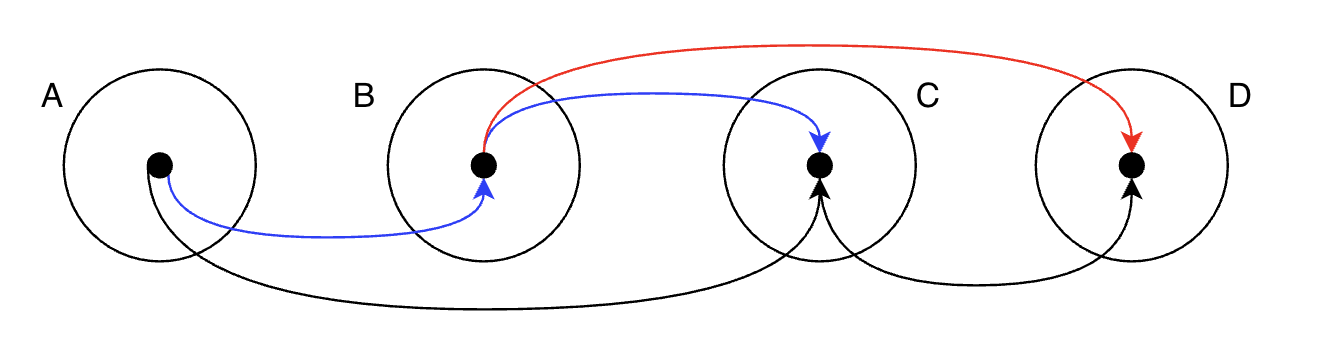
\includegraphics[width=10cm]{dimostrazione-associtiva.png}
            \vspace{-10pt}
            \caption{Rappresentazione dimostrazione 1°}
            \label{fig:rappresentazioni-dim-associtiva}
        \end{figure}
        \\\\
        \underline{Dimostrazione 2°}: R;(S;T) $\subseteq$ (R;S);T\\
        La seconda dimostrazione ha uno svolgimento analoga alla prima. Pure qui andiamo a considerare che: per fare in modo che la prima parte, cioè "R;(S;T)", sia sottoinsieme della seconda, la seconda deve contenere tutti gli elementi della prima. quindi $\forall (a,d) \in R;(S;T) \: \land \:(a,d) \in (R;S);T$. \\ \\Per fare in modo che ciò scritto sia vero dobbiamo dimostrare che $\forall \: (a,d) \in (R;S);T$ sia vero:\\
        Come prima cosa dobbiamo capire in che casi i punti appartengono a "(R;S);T", questo avviene quando esiste un punto "c" che collega "R;S" e "T" (R;S è uguale a A X C e T è C X D), quindi possiamo scrivere che:
        \begin{equation}
            (a,d) \in (R;S);T \Longrightarrow \forall c \in C \: \bullet \: (a,c) \in R;S \land (c,d) \in T
            \label{eq:dim2-associtiva-1}
        \end{equation}
        Da questo punto procediamo come nella dimostrazione 1° quindi andiamo a scomporre ulteriormente la forma [\ref{eq:dim2-associtiva-1}] in $(a,c) \in R;S$ per verificare i casi in cui la composizione esista:
        \begin{equation}
            (a,d) \in (R;S);T \Longrightarrow \: \exists \: b \in B, \: c \in C \: \bullet (a,b) \in R \land (b,c) \in S \land (c,d) \in T
            \label{eq:dim2-associtiva-2}
        \end{equation}
        L'ultimo passaggio è trasformare la forma [\ref{eq:dim2-associtiva-2}] in una versione che possa validare $\forall \: (a,d) \in (R;S);T$, ed essa sarebbe:
        \begin{equation}
            (a,d) \in R;(S;T) \Longrightarrow \: \exists \: c \in C \bullet (a,c) \in R;S \land (c,d) \in T
            \label{eq:dim2-associtiva-3}
        \end{equation}
        L'ultima forma travata [\ref{eq:dim2-associtiva-3}] verifica che $\forall \: (a,d) \in (R;S);T$ sia vero, di conseguenza pure R;(S;T) $\subseteq$ (R;S);T è verificato. $\blacksquare$\\ \\
        Dato che siamo riusciti a dimostrare entrambe le dimostrazioni la proprietà associativa ((R;S);T = R;(S;T)) con cui siamo partiti è verificata. $\blacksquare$
\end{demostration}


\subsection{Proprietà fondamentali}
Prendendo in considerazioni due insiemi $A$ e $B$ ed una relazione R, dove R $\subseteq$ A X B, valgono le seguenti proprietà.\\ \\
%TODO Inserire definizione ed esempi con relazioni già visti (vedi slide)
\textbf{Totale}: $\forall a \in A . (\exists b \in B . (a, b) \in R)$
\hfill
\textbf{Surgettiva}: $\forall \: \: b \in B . (\exists a \in A . (a, b) \in R)$
%TODO La totale e la surgettiva è simmetica
%TODO Acronimo TUSI
\begin{figure}[h!]
    \vspace{-8pt}
    \begin{subfigure}{.3\textwidth}
        \centering
        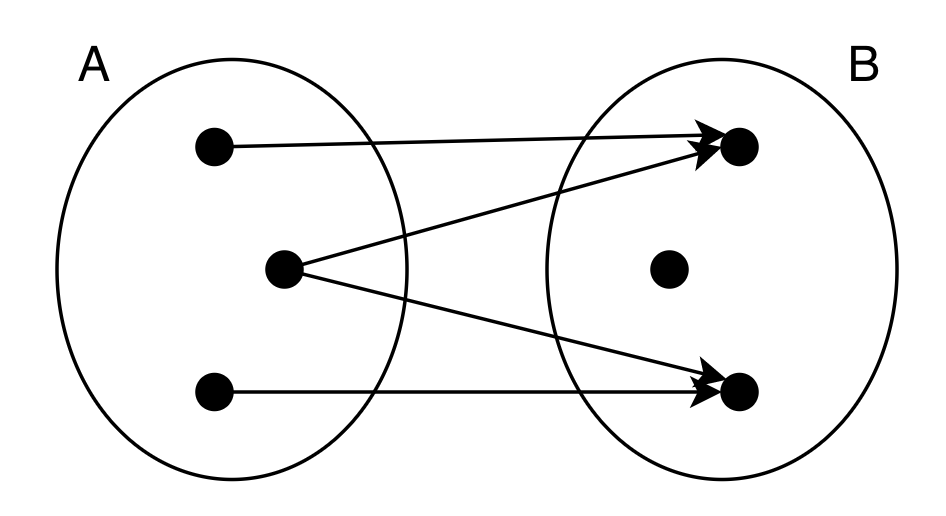
\includegraphics[width=6cm]{totale.png}
        \caption{Ogni elem. di A è collegato ad almeno uno di B}
    \end{subfigure}
    \hspace{4.3cm}
    \begin{subfigure}{.3\textwidth}
        \centering
        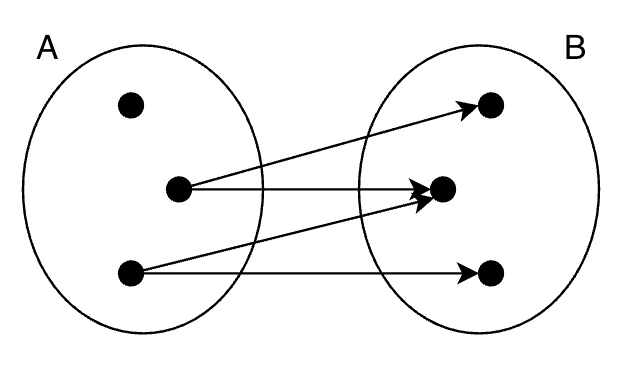
\includegraphics[width=6cm]{surgettiva.png}
        \caption{Ogni elem. di B ha almeno un entrata da A}
    \end{subfigure}
\end{figure}
\\
\textbf{Univalente}: \hspace{6.3cm} \textbf{Iniettiva}:
%TODO Sistemare layout
%TODO Integrare la definizione logica di "al più"
%TODO Aggiungere esempi da relazioni già viste
\\
$\forall a \in A . \exists$ al più un $b \in B . (a, b) \in R$
\hspace{2.4cm} 
$\forall b \in B . \exists$ al più un $a \in A . (a, b) \in R$
\begin{figure}[h!]
    \vspace{-7pt}
    \begin{subfigure}{.3\textwidth}
        \centering
        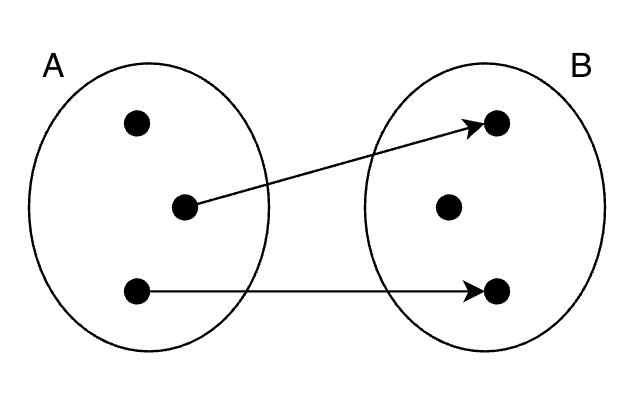
\includegraphics[width=6.2cm]{univalente.png}
        \caption{Ogni elem. di A deve avere al massimo 1 collegamento con B}
    \end{subfigure}
    \hspace{4.3cm}
    \begin{subfigure}{.3\textwidth}
        \centering
        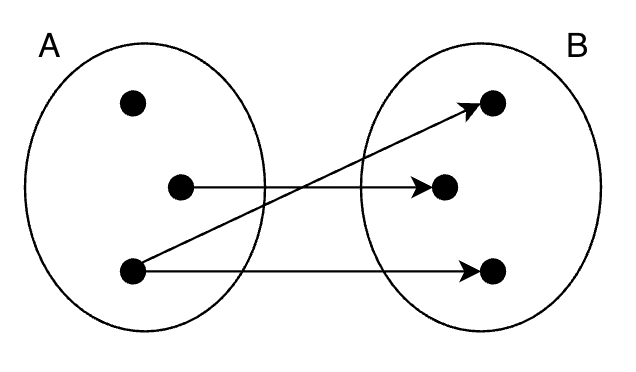
\includegraphics[width=6cm]{iniettiva.png}
        \caption{Ogni elem. di B deve avere al massimo un entrante da A}
    \end{subfigure}
\end{figure}
\\
Le proprietà fra di loro sono legate da un rapporto di \textbf{dualità}:
%TODO inserire link alla proprietà (e.g. totale)
\begin{itemize}
    \item R $\subseteq A \times B$ è totale $\Longleftrightarrow$ $R^{op} \subseteq B \times A$ è surgettiva.
    \item R $\subseteq A \times B$ è surgettiva $\Longleftrightarrow$ $R^{op} \subseteq B \times A$ è totale.
    \item R $\subseteq A \times B$ è univalente $\Longleftrightarrow$ $R^{op} \subseteq B \times A$ è iniettiva.
    \item R $\subseteq A \times B$ è iniettiva $\Longleftrightarrow$ $R^{op} \subseteq B \times A$ è univalente.
\end{itemize}

\subsubsection{Teorema di caratterizzazione}
\label{teorema-caratterizzazione}
%TODO Sistemare le label
Prendendo due insiemi $A$ e $B$ ed una relazione $R$ tale che $R \subseteq A \times B$. Possiamo vedere come ogni proprietà fondamentale vale solo se sono soddisfatte determinate condizioni:
%TODO Aggiungere esempio grafico (slide)
\begin{itemize}
    \item \textbf{Totale} $\Longleftrightarrow Id_A \subseteq R;R^{op}$\\
    La congiunzione fra $R$ che è $A \times B$ e il suo opposto che è $B \times A$ torna un insieme $A \times A$, per questo l'identità di $A$ ($Id_A$), che sarebbe un insieme $A \times A$, è un sottoinsieme di $R;R^{op}$.\\
    Se $R$ non fosse totale vorrebbe dire che alcuni elementi di $R(A)$ non sono collegati.
    
    \item \textbf{Univalente} $\Longleftrightarrow R^{op};R \subseteq Id_B$\\
    La congiunzione fra $R^{op}$ che sarebbe $B \times A$ e $R$, che è $A \times B$, forma un insieme $B \times B$ che è quindi sottoinsieme di $Id_B$, che sarebbe $B \times B$.
    
    \item \textbf{Surgettiva} $\Longleftrightarrow Id_B \subseteq R^{op};R$\\
    La congiunzione fra $R^{op}$ ed $R$, che sono rispettivamente $B \times A$ e $A \times B$, torna una relazione $B \times B$, quindi $Id_B$, che è $B \times B$, è sottoinsieme.
    
    \item \textbf{Iniettiva} $\Longleftrightarrow R;R^{op} \subseteq Id_A$\\
    La congiunzione fra $R$ ed $R^{op}$ torna $A \times A$, essendo che $R$ è $A \times B$ e l'opposto è $B \times A$, che è sottoinsieme di $Id_A$ che è $A \times A$.
\end{itemize}

%TODO Inserire le 2 dimostrazioni del teorema di caratterizzazione (slide) e specificare una nota per "se e solo se" che indica che va dimostrato sia che se A allora B ma anche che se NON A allora NON B

\subsubsection{Proprietà di chiusura per composizione}
Per tutti gli insiemi $A, B, C$ e per tutte le relazioni, $R \subseteq A \times B$ e $S \subseteq B \times C$ vale che:
\begin{enumerate}
    \item Se $R$ ed $S$ sono totali allora la loro composizione $R;S$ è totale.
    \item Se $R$ ed $S$ sono univalenti allora la loro composizione $R;S$ è univalente.
    \item Se $R$ ed $S$ sono surgettive allora la loro composizione $R;S$ è surgettiva.
    \item Se $R$ ed $S$ sono iniettive allora la loro composizione $R;S$ è iniettiva.
\end{enumerate}

\subsection{Funzione}
Una funzione può essere definita utilizzando le proprietà fondamentali delle relazioni.
%TODO Esempi grafici
\begin{definition}[Funzione]
Dati due insiemi $A, B$ ed una relazione $R \subseteq A \times B$, tale relazioni si definisce funzione quando rispetta la proprietà \textbf{totale} e \textbf{univalente} quindi tutti gli elementi dell'insieme $A$ hanno uno ed un solo corrispettivo in $B$.
\end{definition}
\begin{example}
	Ad esempio ne lcaso dei booleani, dato l'insieme $B=\{$true, false$\}$:
	\begin{itemize}
		\item $\neg : B \rightarrow B$ $B = {(t, f), (f, t)}$
		\item $\wedge : B \times B \rightarrow B$
	\end{itemize}
\end{example}

\begin{definition}[Funzione parziale]
    Una funzione si dice parziale se rispetta solamente la proprietà univalente.
\end{definition}
\begin{example}
	Un esempio è la funzione $f:\frac{1}{x}$ con $f: \mathbf{R} \rightarrow \mathbf{R}$
\end{example}

\begin{definition}[Funzioni iniettive e surgettive]
	
\end{definition}

\begin{definition}[Biezione]
Dati due insiemi $A, B$ ed una relazione $R \subseteq A \times B$, tale relazioni si definisce funzione biettiva quando rispetta tutte e 4 le proprietà. Quindi:
\begin{itemize}
	\item $ \forall a \in A$ esiste \textbf{esattamente un} $b \in B . (a, b) \in \mathbf{R}$
	\item $ \forall b \in B$ esiste \textbf{esattamente un} $a \in A . (a, b) \in \mathbf{R}$
\end{itemize}
\end{definition}

\textbf{Domanda:} Se dati due insiemi A, B dove $|A| \neq |B|$ la loro relazione R $\subseteq$ A X B può essere una biezione?\\
La risposta è NO visto che avendo cardinalità diverse esisterà sempre un elemento in B che o non ha corrispettivo o ne ha 2.

\subsubsection{Composizione di funzioni}
\begin{proposition}
	Per tutti gli insiemi $A, B, C$ e tutte le funzioni $f:A\rightarrow B$ e $g:B\rightarrow C$, la relazione $f;g$ è una funzione, $f;g:A \rightarrow C$.
\end{proposition}
\begin{example}
    Dati due funzioni $f$ e $g$ dove:\\
	$f: A \rightarrow B$ \hspace{.5cm} $g: B \rightarrow C$ \footnote{Scrivere una funzione "$f$" nella forma $f: A \rightarrow B$  equivale a scrivere f $\subseteq A \times B$}\\ 
    La compozione si scrive come $f;g$ e sarebbe $f;g \subseteq A \times C$ \footnote{É possibile scrivere la composizione di funzioni anche come $g \cdot f$ oppure $g(f())$}
\end{example}
\begin{note}
	Indichiamo con $fun(A,B) = \{f \mid f: A \rightarrow B\}$ l'insieme di tutte le funzioni che vanno da $A$ a $B$. Di conseguenza $fun(A, B) \subseteq rel(A, B)$.
\end{note}

\subsubsection{Proprietà di chiusura per funzioni}
Per tutti gli insiemi $A, B, C$ e per tutte le relazioni, funzioni, $i: A \rightarrow B$ e $j: B \rightarrow C$ valgono le seguenti proprietà:
\begin{enumerate}
    \item $Id_A$ è una biezione, essendo una relazione con se stesso
    \item Se prendiamo $i: A \rightarrow B$ e $j: B \rightarrow C$, dove entrambe le funzioni sono biezioni, la loro composizione, $i;j: A \rightarrow C$ è a sua volta una biezione
    \item Se prendiamo la funzione $i: A \rightarrow B$ biettiva, il suo opposto $i^{op}: B \rightarrow A$ è a sua volta biettiva
\end{enumerate}

\subsubsection{Caratterizzazione in biezione}\label{caratterizzazione-biezione}
Per tutti gli insiemi $A, B$, per tutte le relazioni $R: A\leftrightarrow B$ vale che:
\begin{itemize}
	\item $R$ è una biiezione se e solo se $Id_A = R;R^{op}$ e $Id_B = R^{op};R$
	\item Una relazione $S:B\leftrightarrow A$ è l'inversa di $R$ se $Id_A = R;S$ e $Id_B = S;R$
	\item $R:A\leftrightarrow B$
\end{itemize}

\textbf{Spiegazione:} Per definire la proprietà di caratterizzazione per una relazione biettiva bisogna partire da cos'è una relazione biettiva: una relazione è biezione quando è contemporaneamente totale, univalente, surgettiva ed iniettiva. \\Da qui capiamo che se una relazione ha tutte e 4 le proprietà a suo volta dovrà rispettare per ciascuna di esse la caratterizzazione associata vista nel paragrafo \ref{teorema-caratterizzazione}. \\Quindi semplicemente riscriviamo questa quattro proprietà semplificando $Id_A \subseteq R;R^{op}$ con $R;R^{op} \subseteq Id_A$ in $Id_A = R;R^{op}$ e $Id_B \subseteq R^{op};$ con $R^{op};R \subseteq Id_B$ con $Id_B = R^{op};R$ (possiamo fare questa "semplificazione" perché due insiemi sono uguali quando uno è sottoinsieme dell'altro, come in questo caso).
\begin{example}
    Come si usa la caratterizzazione:\\
    Dati due insiemi A, B ed una relazione R $\subseteq$ A X B. Se riusciamo a trovare una relazione S $\subseteq$ B X A tale che venga soddisfatta la definizione sopra scritta per cui $Id_A = R;S \land S;R = Id_B$ è equivalente a dimostrare che la relazione R è una biezione.
\end{example}

\subsubsection{Insiemi di biezione}
\begin{definition}[Insiemi di biezione]
Dati due insiemi A e B, essi sono in biezione
\footnote{puoi chiamare due insiemi in biezione anche in corrispondenza, 1-1 o in una relazione biunivoca}
se esiste una biezione $i: A \rightarrow B$, e si scrive come $A \cong B$
\footnote{attenzione: usare il simbolo $\cong$ invece che un semplice = vuole dire che non per forza le due parti devono essere ugualia}
\end{definition}
\begin{example}
    Esempi insiemi di biezione:
    \begin{itemize}
        \item Dati gli insiemi $2 = \{0,1\}$ e bool = $\{true, false\}$ \hspace{.3cm} l'insieme di biezione è $2 \cong$ bool
        \item Dati A e B \hspace{.3cm} l'insieme di biezione è A $\times$ B $\cong$ B $\times$ A \\
        Altri modi per scriverlo sono: \hspace{.3cm} i:A $\times$ B $\longrightarrow$ B $\times$ A \: - \: i((a,b))=(b,a)\footnote{questa forma vuol dire che se diamo in input alla funzione i una coppia di valori (a,b) restituirà una coppia (b,a)}\\
        \textbf{NOTA:} A $\times$ B = B $\times$ A sarebbe farlo perché uno crea coppie (a,b) e l'altro coppie (b,a).
        \item Dati gli insieme $1 = \{0\}$ ed A \hspace{.3cm} l'insieme di biezione è A $\times$ 1 $\cong$ A \\
        Altri modi per scriverlo sono: \hspace{.3cm} i:A $\times$ 1 $\longrightarrow$ A \hspace{.3cm} i((a,0)) = a
        \item fun(A $\times$ B, C) $\cong$ fun(A, (fun(B,C))\\
        \textbf{Spiegazione esempio:} la prima funzione data una coppia (a,b) restituisce un valore c mentre la seconda funzione dando un valore a restituisce una nuova funzione, dove a sua volta se inseriamo un valore b restituisce c. Quindi f((a,b)) = c e f(a)(b)=c.
    \end{itemize}
\end{example}
\begin{example} Esempio particolare con dimostrazione \\
        Per tutti gli insiemi $A, B, C$ vale che:
        \begin{equation}
            (A \times B) \times C \cong A \times (B \times C)
        \end{equation}
        \begin{demostration}
            Innanzitutto scriviamo questa biezione sotto la seguente forma \\i((a,b),c) = (a,(b,c)) dove la funzione "i" prende in input una coppia di valori ((a,b),c) e restituisce (a,(b,c)).\\
            Utilizziamo la proprietà di caratterizzazione scritta nel paragrafo \ref{caratterizzazione-biezione} che dice che: \\ $R \Longleftrightarrow Id_A = R;R^{op} \land Id_B = R^{op};R$.\\
            Sfruttiamola applicandola al nostro caso quindi (consideriamo i come una relazione fra due insiemi W e K dove W è $((A \times B) \times C)$ e K è $(A \times (B \times C)))$:
            \begin{equation}
                i \: \: biettiva \Longleftrightarrow Id_W = i;i^{op} \land i^{op};i = Id_K
            \end{equation}
            Il nostro obbiettivo è quindi trovare $i^{op}$ che soddisfi le due condizioni determinate da $\land$ sopra:
            \begin{itemize}
                \item $Id_W = i;i^{op}$ - \underline{Dimostrazione 1°}
                \item $Id_K = i^{op};i$ - \underline{Dimostrazione 2°}
            \end{itemize}
                \underline{Dimostrazione 1°} - $Id_W = i;i^{op}$
                Ricordiamo che l'opposto di "i" è $i^{op}: A \times (B \times C) \longrightarrow (A \times B) \times C$ che quindi possiamo vedere come una funzione che prende in ingresso una coppia di valori (a, (b,c)) e restituisce ((a,b),c).\\
                Ora rappresentiamo la composizione fra i e $i^{op}$ come unione fra funzioni come funzione di una funzione quindi: $i;i^{op} = i^{op}(i(x))$\\
                Ora semplicemente riscriviamo la composizione di funzioni scrivendo i parametri di input ed output:
                \begin{equation}
                    i^{op}(i((a,b),c) = i^{op}(a, (b,c)) \: \: che \: \: restituisce \: \: ((a,b),c)
                \end{equation}
                Vediamo così che l'opposto di i restituisce lo stesso valore che restituisce $Id_W$ ($Id_W$ è una relazione fra W e W, visto che W è (A $\times$ B) $\times$ C possiamo scrivere che $Id_W((a,b),c) = ((a, b),c)$).
                \item $\mathcal{P}(A) \cong$ fun(A,2)\footnote{Questo insieme è quello dei numeri binari}. Questo caso è dimostrato. $\blacksquare$\\ \\
                \underline{Dimostrazione 2°} - $Id_K = i^{op};i$
                Procediamo in maniera analoga alla dimostrazione 1° quindi andiamo a rappresentare la composizione fra l'opposto $i^{op}$ ed i come funzioni di funzione $i(i^{op})$ andando poi ad inserire i parametri i input ed output:
                \begin{equation}
                    i(i^{op}(a,(b,c)) = i((a,b),c) \: \: che \: \: restituisce \: \: (a, (b,c))
                \end{equation}
                Pure in questo caso possiamo vedere che l'opposto di K $Id_K$ restituisce gli stessi valori scritti sopra (anche in questo caso tieni a mente che l'opposto di $Id_K$ è una relazione che associa K con K quindi, ricordando che K è A $\times$ (B $\times$ C), se la scriviamo sotto forma di funzione è $Id_K(a,(b,c)) = (a,(b,c)$). Anche questo caso è dimostrato. $\blacksquare$\\ \\
                Essendo che entrambi le casistiche sono state dimostrate possiamo concludere che l'insieme di biezione (A $\times$ B) $\times$ C $\cong$ A $\times$ (B $\times$ C) è dimostrato. $\blacksquare$
        \end{demostration}
\end{example}

\subsubsection{Proprietà insiemi di biezione}
Per tutti gli insiemi $A, B, C$ valgono le proprietà scritte nella tabella \ref{tab:proprietà-insiemi-biezione}.
\begin{table}[h!]
    \centering
    \setlength{\tabcolsep}{8pt}
    \renewcommand{\arraystretch}{2}
    \begin{tabular}{|c|c|}
    \hline
        \textbf{Riflessiva} & A $\cong$ A  \\
        \textbf{Simmetrica} & A $\cong B \Longrightarrow B \cong A$ \\
        \textbf{Transitiva} & $A \cong B$, $B \cong C \Longrightarrow A \cong C$\\ \hline
    \end{tabular}
    \caption{Proprietà insiemi di biezione}
    \label{tab:proprietà-insiemi-biezione}
\end{table}

\subsection{N-upla}
\begin{definition}[N-upla]
Sia $A$ un insieme e $n \in \mathbf{N}$. Una sequenza su $A$ di lunghezza $n$ è una n-upla ($a_0, a_1, \ldots, a_{n-1}$) dove $a_i \in A$ per ogni indice $i \in \{0,1,\ldots,n-1\}$. Definiamo quindi l'insieme $A^n$ du tutte le sequenze come:
\begin{equation}
    A^n = \{(a_0,a_1, ..., a_{n+1}) \:|\: \forall \: i \in \{0,...,n-1\}\:.\: a_i \in A\}
\end{equation}
\end{definition}

\begin{definition}[Sequenza su A di lunghezza arbitraria]
Una sequenza su A di lunghezza arbitraria è una sequenza di lunghezza n per qualsiasi numero naturale $n \in \mathbb{N}$. L'insieme di tutte le sequenze su A di lunghezza arbitraria:
\[A^* = \bigcup_{n\in \mathbb{N}} A^n\]
\end{definition}
\newpage
\section{Induzione}
L'induzione è un metodo formale che aiuta a definire in modo rigoroso insiemi, funzioni ma anche serve per dimostrare che una proprietà è vera per tutti gli elementi di un tale insieme. Diventa sopratutto unitile quando queste definizioni sono un insiemi, funzioni di cardinalità o di lunghezza notevolmente grande (ma sempre finiti).
\subsection{Schema generale induttivo}
Schema generare induttivo usato per definire un insieme A, e con il quale tramite una regola finita andiamo a rappresentare infinite soluzioni:
\begin{enumerate}
    \item \textbf{Clausola base}, o caso base, che stabilisce che certi oggetti appartengono all'insieme. Questi elementi costituiscono i mattoncini per costruire altri elementi dell’insieme. Nel nostro caso andiamo ad elencare un numero finito di elementi che appartengono ad A.
    \item \textbf{Clausola induttiva} o passo induttivo, che descrive in che modo gli elementi dell'insieme possono essere usati per produrre altri elementi dell'insieme. Nel nostro caso usiamo elementi di A per costruirne o definirne altri.
    \item \textbf{Clausola terminale}, che stabilisce che l'insieme che si sta definendo non contiene altri elementi oltre a quelli ottenuti dalle due clausole precedenti. Quindi l'insieme definito è il più piccolo insieme che soddisfa la clausola base e quella induttiva. Nel nostro caso definiamo che gli unici elementi che soddisfano A sono quelli definiti nelle condizioni 1 e 2. \footnote{La clausola terminale di solito non viene specificata essendo sotto intesa}
\end{enumerate}
\begin{example}
    Riscrivendo per intero in nostro esempio con A:\\
    \underline{Clausola base:} $A_1$ X $A_2$ è una n-upla\\
    \underline{Clausola induttiva:} $A_1$ X $A_2$ X $A_3$ è una n-upla\\ \\
    Tramite queste due clausole possiamo andare a ricreare ogni n-upla (2-upla, 3-upla, ecc..) andando semplicemente a ripetere la clausola induttiva partendo da quella base. Infatti una 3-upla è clausola base per 1 volta clausola induttiva, mentre una 4-upla è la clausola base più due ripetizioni della clausola induttiva: \\
    3-upla = $A_1$ X $A_2$ X $A_3$ \hspace{.5cm} 4-upla = $A_1$ X $A_2$ X $A_3$ X $A_4$ \hspace{.5cm} e così per ogni n-upla
\end{example}
\begin{example}
    Altri esempi particolari di casi induttivi:
    \begin{itemize}
        \item \textbf{Chiusura di kleene} o stella di kleene: $A^{*} = \bigcup\limits_{n=0}^{\infty} A^n$ \hspace{.3cm} $A^n =$ A X A x A ... (n volte).\\
        Parte da 0 perché si considera quella che in informatica sarebbe la stringa vuota, cioè $A^0 = \{\}$, che si rappresentata con $\epsilon$.
        \item \textbf{Chiusura positiva}: $A^{+} = \bigcup\limits_{n=1}^{\infty} A^n$ \hspace{.3cm} Uguale alla stella di kleene ma senza insieme vuoto.
    \end{itemize}
    Entrambi questi casi sono operazioni molto consuete nel mondo dell'informatica, essendo che possiamo vedere A come un insieme di caratteri per esempio A = unicode, e tramite queste operazioni si vanno a creare tutte le possibili sequenze o stringhe con quei caratteri.
\end{example}

\subsection{Definizione induttiva dell'insieme $\mathbb{N}$}
\begin{definition}[Definizione induttiva insieme $\mathbb{N}$]\label{definizioni-induttiva-insieme-N}
    L’insieme N dei numeri naturali è l’insieme di numeri che soddisfa le seguenti clausole:
    \begin{enumerate}
        \item \underline{Clausola base:} $0 \in \mathbb{N}$.
        \item \underline{Clausola induttiva:} se $n \in \mathbb{N}$ allora $(n + 1) \in \mathbb{N}$.
    \end{enumerate}
\end{definition}
Definendo le tre clausole è immediato capire la definizione dell'insieme $\mathbb{N}$ per induzione. Infatti possiamo ricavare qualsiasi numero dell'insieme semplicemente partendo da 0 (che già sappiamo per clausola base appartenere all'insieme) e ripetendo la clausola induttiva tante volta quanto mi serve. 

\begin{example}
    Altri esempi analoghi alla definizione dell'insieme $\mathbb{N}$:
    \begin{enumerate}
        \item Definizione \textbf{N. pari}: \hspace{.3cm} \underline{Base:} $2 \in \mathbb{N}^{pari}$ \hspace{.3cm} \underline{Induttiva:} se $n \in \mathbb{N}^{pari}$ allora $n+2 \in \mathbb{N}^{pari}$
        \item Definizione \textbf{N. dispari}: \hspace{.1cm} \underline{Base:} $1 \in \mathbb{N}^{dispari}$ \hspace{.2cm} \underline{Induttiva:} se $n \in \mathbb{N}^{dispari}$ allora $n+2 \in \mathbb{N}^{dispari}$
        \item Definizione \textbf{Potenze 2}: \hspace{.2cm} \underline{Base:} $1 \in$ P \hspace{.2cm} \underline{Induttiva:} se $p \in$ P allora $2*p \in$ P
        
        È possibile scrivere anche come: \hspace{.2cm} \underline{Base:} $2^0 \in P$ \hspace{.2cm} \underline{Induttiva:} se $2^n \in P$ allora $2^n+1 \in P$
    \end{enumerate}
\end{example}

\subsection{Definizione induttiva di funzioni}
Per andare ad effettuare la definizione induttiva di una funzione bisogna andare (1) a stabilire il valore delle funzioni per gli elementi appartenenti alla clausola base e (2) una regola per andare a calcolare il valore della funzione sugli elementi che vi appartengono, stabiliti dalla clausola induttiva. Successivamente tramiti te la clausola terminale definiamo che i punti (1) e (2) sono sufficienti a definire la funzione per tutti gli elementi dell'insieme. Quindi, prendendo una $f: A \longrightarrow B$:
\begin{itemize}
    \item La \textbf{clausola base} sarà il valore di f(a) per alcuni $a \in A$.
    \item La \textbf{clausola induttiva} invece indicherà il valore di f(a) utilizzando valori di f già definiti in precedenza.
\end{itemize}
\begin{example}
    Facciamo un primo esempio definendo la funzione dei \textbf{numeri triangolari}.
    \begin{definition}[Numeri triangolari]
        Per ogni $n \in \mathbb{N}$ in numero triangolare $T_n$ è uguale alla somma di tutti i numeri minori o uguali a n:
        \begin{equation}\label{numeri-triangolari}
            T_n: \mathbb{N} \longrightarrow \mathbb{N} \: \: \: o \: \: \: T_n = fun(\mathbb{N},\mathbb{N}) \hspace{1cm} T_n = \sum_{\substack{i=0}}^n i
        \end{equation}
    \end{definition}
    \begin{enumerate}
        \item \underline{Clausola base:} $T_0 = 0$
        \item \underline{Passo induttivo:} $T_{n + 1} = T_n + (n + 1)$
    \end{enumerate}
    Per andare a dimostrare questa casistica possiamo procedere per casi andando a controllare $n=1, n=2, n=3, ...$ e dimostrare la validità per questi casi, cosa che però non porta ad un risultato per un generico numero $n$. Per dimostrare la validità bisogna andare a dimostrare quella che vine chiamata \textit{formula di gauss}.
    \begin{equation}\label{formula-gauss}
        \forall\: \: n \in \mathbb{N} \: . \: \bigg(T_n = \frac{n \cdot (n + 1)}{2}\bigg)
    \end{equation}
\end{example}

\subsection{Dimostrazione induttiva di proprietà}
Per andare a dimostrare una proprietà bisogna applicare il principio di induzione sui numeri naturali, che, dato una generica proprietà $P(n)$ sui naturali dice:
\begin{definition}[\textbf{Principio di induzione}]
    Se (caso base) $P(0)$ è vera, e se (passo induttivo) per ogni $n \in \mathbb{N}$ vale che se $P(n)$ è vera allora anche $P(n+1)$ lo è, allora $P(m)$ è vera per ogni $m \in \mathbb{N}$
    \begin{equation}
        \frac{P(0) \: \: \: \forall \: \: n \in \mathbb{N}\:.\:(P(n) \Longrightarrow P(n+1)}{\forall \: \: m \in \mathbb{N}\:.\:P(m)}
    \end{equation}
\end{definition}
\begin{proposition}[Formula di gauss]
La formula (\ref{formula-gauss}), $T_n = \frac{n \cdot (n + 1)}{2}$, è valida per ogni $n \in \mathbb{N}$
\end{proposition}
\begin{demostration}[Formula di gauss]
Per dimostrare la formula di gauss (\ref{formula-gauss}) per induzione è sufficiente dimostrare i seguenti casi:
\begin{enumerate}
    \item \underline{Caso base:} $T_0 = 0$, perché per definizione sarebbe $\frac{0 \cdot (0 + 1)}{2} = 0$, quindi la formula di gauss (\ref{formula-gauss}) per $n = 0$ è vera.
    \item \underline{Passo induttivo:} Assumiamo che l'ipotesi $T_n = \frac{n \cdot (n + 1)}{2}$ sia vera e dimostriamo che è vera per ogni $n + 1$, cioè che:\\\\
    $T_{n+1} = T_n + (n + 1)$ \hspace{.5cm} Possibile per il passo induttivo della definizione dei numeri triangolari \ref{numeri-triangolari} \\\\
    $= \frac{n \cdot (n + 1)}{2} + (n + 1)$ \hspace{.5cm} Sostituiamo a $T_n$ la clausola induttiva\\\\
    $= \frac{n \cdot (n + 1) + 2 \cdot (n + 1)}{2}$ \hspace{.5cm} Sviluppiamo l'equazione\\\\
    $= \frac{(n + 2) \cdot (n + 1)}{2}$  \hspace{.5cm} Dimostrato il caso $T_{n+1}$ la formula è dimostrata per induzione. \: \: $\blacksquare$
\end{enumerate}
\end{demostration}
\begin{example}[De Morgan]
    Facciamo un altro esempio andando a dimostrare la proprietà di \textbf{De Morgan} per induzione. Tale proprietà dice che:
    \begin{center}
        $\overline{(A \cup B)} = \overline{A} \cap \overline{B}$
    \end{center}
    Noi dobbiamo andare a dimostrare che questa legge può vale per più insiemi utilizzando l'induzione. Quindi dobbiamo far valere la generalizzazione:
    \begin{center}
        $DM(n) = \forall \: \: A_1, ..., A_n \: \cdot \: \Bigg(\overline{\Big( \bigcup\limits_{i=1}^{n} A_i \Big)} = \bigcap\limits_{i=1}^{n}\overline{A_i} \Bigg)$
    \end{center}
    Noi a questo punto dobbiamo in particolare andare a dimostrare che per ogni $n \geq 2$ vale $DM(n)$:
    \begin{center}
        $\forall\: \: n \: . \: (n \geq 2 \Longrightarrow DM(n))$
    \end{center}
    \begin{enumerate}
        \item \underline{Caso base:} $DM(2)$ diche che $\overline{(A_1 \cup A_2)} = \overline{A_1} \cap \overline{A_2}$, ed è dimostrato perché è ciò che dice la legge di De Morgan.
        \item \underline{Passo induttivo:} Assumiamo che $DM(n)$ sia vera e dimostriamo che vale anche $DM(n+1)$. Noi quindi vogliamo dimostrare che la seguente proprietà sia vera:
        \begin{center}
            $DM(n+1) = \forall \: \: A_1, ..., A_{n+1} \: \cdot \: \Bigg(\overline{\Big( \bigcup\limits_{i=1}^{n+1} A_i \Big)} = \bigcap\limits_{i=1}^{n+1}\overline{A_i} \Bigg)$
        \end{center}
        Se prendiamo $n+1$ che è un insieme di $A_1, A_2, ...A_n, A_{n+1}$ notiamo che:\\ \\
        $\overline{\Big( \bigcup\limits_{i=1}^{n+1} A_i \Big)} = \overline{\Big(A_{n+1} \cup \bigcup\limits_{i=1}^{n} A_i \Big)}$ \hspace{.5cm} Perché possiamo usare la proprietà associativa per $\cup$.\\ \\
        $= \overline{A_{n+1}} \cap \overline{\Big(\bigcup\limits_{i=1}^{n} A_i \Big)}$ \hspace{.5cm} Utilizzando De Morgan\\\\
        $= \overline{A_{n+1}} \cap \Big(\bigcap\limits_{i=1}^{n} \overline{A_i} \Big)$ \hspace{.5cm} Per ipotesi induttiva.\\\\
        $= \Big(\bigcup\limits_{i=1}^{n+1} \overline{A_i} \Big)$ \hspace{.5cm} Possiamo racchiudere tutto sotto la concatenazioni di intersezioni. \\ \\
        Vediamo quindi che anche il $DM(n+1)$ è dimostrato, quindi che tutte le sequenze $DM(n)$ sono dimostrate. \: \: $\blacksquare$
    \end{enumerate}
\end{example}
\begin{example}[Numeri di Fibonacci]
    La successione dei numeri di Fibonacci può essere definita induttivamente come:
    \begin{enumerate}
        \item $f_1 = 1$
        \item $f_2 = 1$
        \item $f_n = f_{n-1} + f_{n-2}$ \hspace{.5cm} se $n > 2$
    \end{enumerate}
    \begin{demostration}[Numeri di Fibonacci]
        Proviamo a dimostrare questa successione numerica. Sia $f_i$ l'i-esimo numero di Fibonacci, noi dobbiamo dimostrare per induzione che:
        \begin{equation}
            \forall \: \: n \in \mathbb{N}^{+}\:.\: \bigg(\sum_{\substack{i=1}}^n f_i^2 = f_n \: \cdot \:f_{n+1} \bigg)
        \end{equation}
        \begin{enumerate}
            \item \underline{Caso base:} Poiché noi dobbiamo dimostrare per tutti gli $n$ tale che $n \in \mathbb{N}^{+}$ per il caso base dobbiamo considerare $n = 1$, quindi il nostro caso base sarà $\sum_{i=1}^1\:f_i^{2} = f_1 \: \cdot \: f_{2}$. questo caso è dimostriamo immediatamente dalla definizione di $f_i$
            \item \underline{Passo induttivo:} Assumiamo per ipotesi induttiva che valga $\sum_{i=1}^n\:f_i^{2} = f_n \: \cdot \: f_{n+1}$
        \end{enumerate}
        Una volta assunto per vero il passo induttivo possiamo dimostrare il caso $n+1$, ciò porta a dimostrare che:\\ \\
        $\sum_{i=1}^{n+1}\:f_i^{2} = \sum_{i=1}^{n}\:f_n^2 \: + \: f_{n+1}^2$ \hspace{.3cm} Togliamo l'ultimo termine dalla sommatoria e scriviamolo esplicitamente. \\ \\
        $= f_n^2 \: \cdot \: f_{n+1}^2 + \: f_{n+1}^2$ \hspace{.3cm} Applichiamo l'ipotesi induttiva \\ \\
        $= (f_n^2 \: + \: f_{n+1}^2) \: \cdot \: f_{n+1}$  \hspace{.3cm} Proprietà distributiva\\ \\
        $= f_{n+2}^2 \: \cdot \: f_{n+1}$  \hspace{.3cm} Sviluppiamo l'equazione \\\\
        Vediamo come $f_{n+2}^2 \: \cdot \: f_{n+1}$ sia la causala induttiva che volevamo dimostrare. Possiamo dire dunque che la formula di Fibonacci e dimostrata. $\blacksquare$
    \end{demostration}
\end{example}

\subsection{Principio di Induzione forte sui naturali}
Il Principio di Induzione Forte sui naturali ci permette di rafforzare le ipotesi del passo induttivo e portare avanti la dimostrazione in modo più semplice.
\begin{definition}[Induzione Forte]
    Se per ogni $n \in \mathbb{N}$ vale che se P(0), P(1),..., P(n-1) sono vere allora anche P(n) lo è, allora P(m) è vera per ogni $m \in \mathbb{N}$.
    \begin{equation}
        \frac{\forall n . (P(0) \: \land P(1) \land ... \land P(n-1) \rightarrow P(n))}{\forall m . P(m)}
    \end{equation}
\end{definition}
\newpage
\section{Relazioni su un insieme}
\begin{definition}[Relazioni su un insieme]
Dato un insieme A, una relazione su un insieme A è un sottoinsieme A X A, cioè un elemento di rel(A,A), dove rel(A,A) è l'insieme delle possibili relazioni A X A. Quindi una relazione $R \subseteq$ A X A.
\end{definition}
Le relazioni su insiemi sono caratterizzate dal fatto che si sviluppano fra due insiemi uguali. Infatti non è una relazione su un insieme un $R \subseteq$ A X B.
\begin{example}
Alcuni esempi generali di relazioni su un insieme:
\begin{itemize}
    \item Succ = $\{(x,y) \in \mathbb{N}$ X $\mathbb{N}\: \setminus\: y=x+1\}$
    \item $id_A \in$ rel(A,A) è una relazione su A
    \item S è l'insieme degli studenti. CompagnoDiClasse $\in$ rel(S,S)
    \item Somma $\in$ rel(($\mathbb{Z}, \mathbb{Z}$), $\mathbb{Z}$) Somma non è una relazione su in inseme.
\end{itemize}
\end{example}

\subsection{Proprietà di relazione su un insieme}
\subsubsection{Riflessiva}
Dato un inseme A, una relazione $R: A \longleftrightarrow A$ possiamo definirla come:
\begin{definition}[Riflessiva]
    R è una relazione \textbf{riflessiva} se per tutti gli $a \in A$ vale che $(a, a) \in R$
    \begin{center}
        $\forall \: a \in A . (a, a) \in R$
    \end{center}
\end{definition}
Rappresentiamo \textbf{graficamente} ora una relazione riflessiva. \\Dato un insieme A di partenza dove A = $\{a, b, c, d\}$:
\begin{itemize}
    \item Il caso [\ref{fig:relazione-riflessiva}] è riflessivo perché ogni elemento è collegato a se stesso \footnote{Il collegamento di un elemento a se stesso viene anche chiamata cappio}.
    \item Il caso [\ref{fig:relazione-non-riflessiva}] non è riflessivo perché gli elementi $c$ e $b$ non sono collegati con loro stesso.
\end{itemize}
\begin{figure}[h!]
    \vspace{-15pt}
    \centering
    \begin{subfigure}{.3\textwidth}
        \centering
        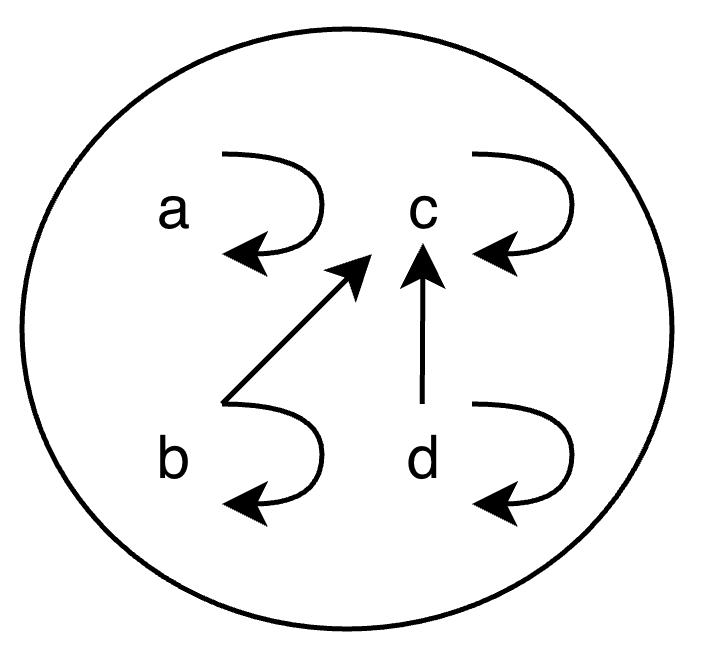
\includegraphics[width=3cm]{images/relazione-riflessiva.png}
        \caption{Relazione riflessiva}
        \label{fig:relazione-riflessiva}
    \end{subfigure}
    \hspace{1.5cm}
    \begin{subfigure}{.3\textwidth}
        \centering
        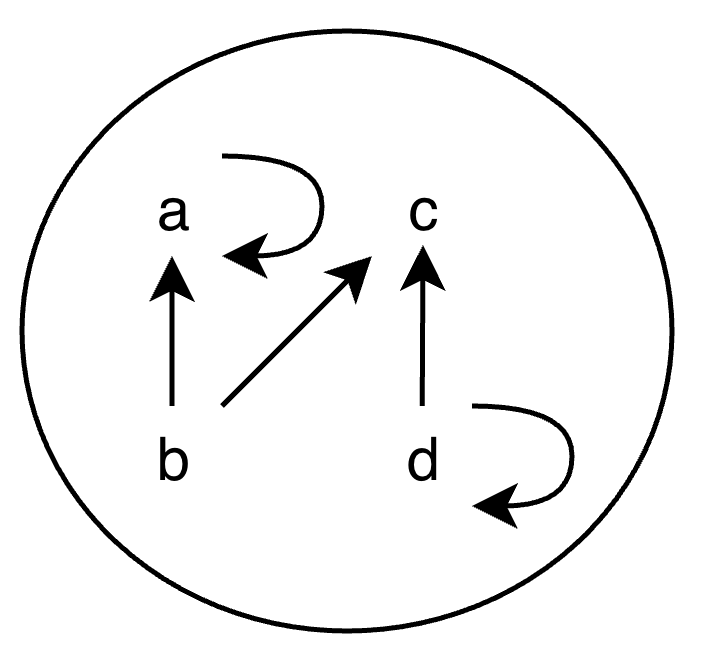
\includegraphics[width=3cm]{images/relazione-non-riflessiva.png}
        \caption{Relazione non riflessiva}
        \label{fig:relazione-non-riflessiva}
    \end{subfigure}
\end{figure}
\begin{example}
Alcuni esempi di relazioni riflessive:
    \begin{itemize}
        \item L'Identità di A $Id_A: A \longleftrightarrow A$ è riflessiva.
        \item La relazione completa $A$ X $A:A \longleftrightarrow A$ è riflessiva.
        \item La relazione vuota $\O: A \longleftrightarrow A$ non è riflessiva perché non ci sono relazioni fra elementi.
        \item La relazione minore $<: \mathbb{N} \longleftrightarrow \mathbb{N}$ \footnote{La relazione minore è definita come: $< = \{(x,y) \in \mathbb{N}$ X $\mathbb{N}\:|\: x < y\}$} non è riflessiva perché un numero non è minore di se stesso.
        \item La relazione minore-uguale $\leq: \mathbb{N} \longleftrightarrow \mathbb{N}$ \footnote{La relazione minore-uguale è definita come: $\leq = \{(x,y) \in \mathbb{N}$ X $\mathbb{N}\:|\: x \leq y\}$} è riflessiva.
        \item La relazione madre:EU $\longleftrightarrow$ EU non è riflessiva.
    \end{itemize}
\end{example}

\newpage
\subsubsection{Simmetrica}
Dato un inseme A, una relazione $R: A \longleftrightarrow A$ possiamo definirla come:
\begin{definition}[Simmetrica]
    R è una relazione \textbf{simmetrica} se per tutti gli $a,b \in A$ vale che se $(a, b) \in R$ allora $(b,a) \in R$.
    \begin{center}
        $\forall \: a,b \in A . (a, b) \in R \Longrightarrow (b,a) \in R$
    \end{center}
\end{definition}
Rappresentiamo \textbf{graficamente} ora una relazione simmetrica. \\Dato un insieme A di partenza dove A = $\{a, b, c, d\}$:
\begin{itemize}
    \item Il caso [\ref{fig:relazione-simmetrica}] è simmetrica perché ogni elemento esiste la coppia inversa di ogni collegamento.
    \item Il caso [\ref{fig:relazione-non-simmetrica}] non è simmetrica perché gli elementi $c$ e $d$ hanno un collegamento sono in un verso.
\end{itemize}
\begin{figure}[h!]
    \vspace{-10pt}
    \centering
    \begin{subfigure}{.3\textwidth}
        \centering
        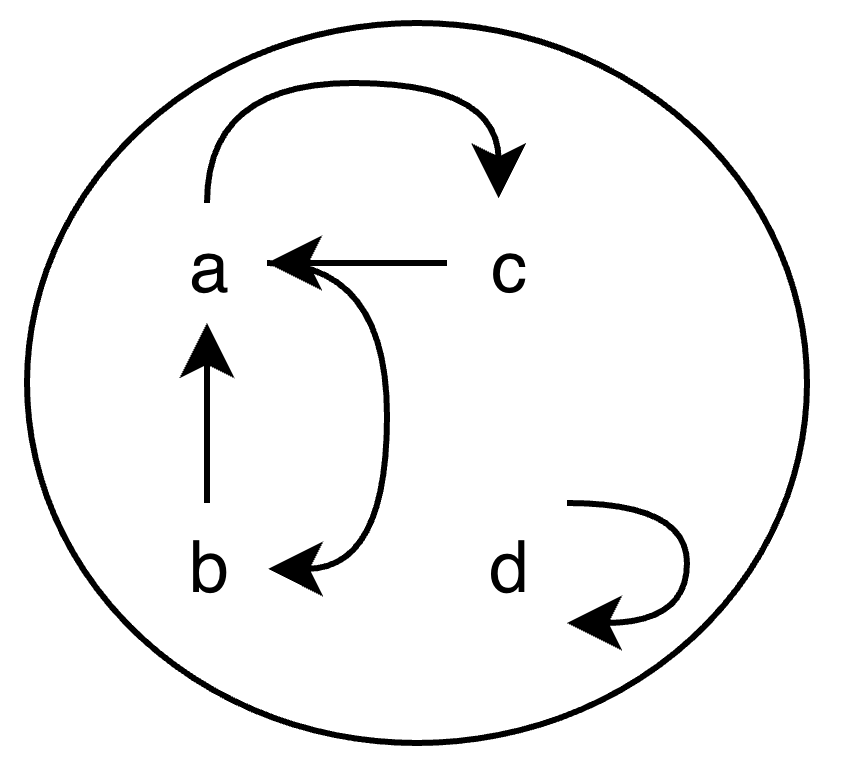
\includegraphics[width=3cm]{images/relazione-simmetrica.png}
        \caption{Relazione simmetrica}
        \label{fig:relazione-simmetrica}
    \end{subfigure}
    \hspace{1.5cm}
    \begin{subfigure}{.3\textwidth}
        \centering
        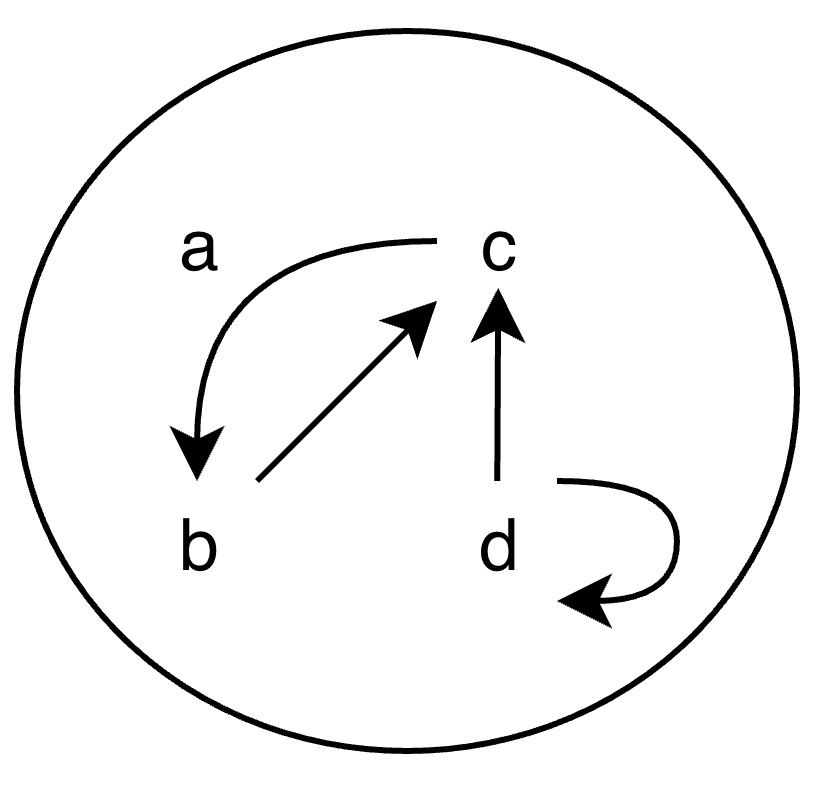
\includegraphics[width=3cm]{images/relazione-non-simmetrica.png}
        \caption{Relazione non simmetrica}
        \label{fig:relazione-non-simmetrica}
    \end{subfigure}
\end{figure}
\begin{example}
Alcuni esempi di relazioni simmetrica:
    \begin{itemize}
        \item L'Identità di A $Id_A: A \longleftrightarrow A$ è simmetrica.
        \item La relazione completa $A$ X $A:A \longleftrightarrow A$ è simmetrica.
        \item La relazione vuota $\O: A \longleftrightarrow A$ è simmetrica.
        \item La relazione minore $<: \mathbb{N} \longleftrightarrow \mathbb{N}$ non è simmetrica perché se un elemento $a$ è minore di un elemento $b$ non può essere che esista l'inverso.
        \item La relazione minore-uguale $\leq: \mathbb{N} \longleftrightarrow \mathbb{N}$ non è riflessiva perché ci sono casi in cui $a$ è minore di un elemento $b$ che non permettono l'inverso.
        \item La relazioni di amicizia su facebook FbFreind:FB $\longleftrightarrow$ FB è simmetrica.
        \item La relazioni di follow su instagram IGFollow:IG $\longleftrightarrow$ IG non è simmetrica perchè se te sei follow di un utente questo utente non necessariamente lo è di te.
    \end{itemize}
\end{example}

\subsubsection{Transitiva}
Dato un inseme A, una relazione $R: A \longleftrightarrow A$ possiamo definirla come:
\begin{definition}[Transitiva]
    R è una relazione \textbf{transitiva} se per tutti gli $a,b,c \in A$ vale che se $(a, b) \in R$ e $(b, c) \in R$ allora $(a, c) \in R$
    \begin{center}
        $\forall \: a,b,c \in A . (a, b) \in R \land (b, c) \in R \Longrightarrow (a,c) \in R$
    \end{center}
\end{definition}
Rappresentiamo \textbf{graficamente} ora una relazione transitiva. \\Dato un insieme A di partenza dove A = $\{a, b, c, d\}$:
\begin{itemize}
    \item Il caso [\ref{fig:relazione-transitiva}] è transitiva perché ogni caso in cui un elemento che si trova "nel mezzo" fra due altri elementi prevede un collegamento fra questi due elementi.
    \item Il caso [\ref{fig:relazione-non-transitiva}] non è transitiva perché esiste (d,c) e (c,a) ma non (a,c).
\end{itemize}
\begin{figure}[h!]
    \vspace{-10pt}
    \centering
    \begin{subfigure}{.3\textwidth}
        \centering
        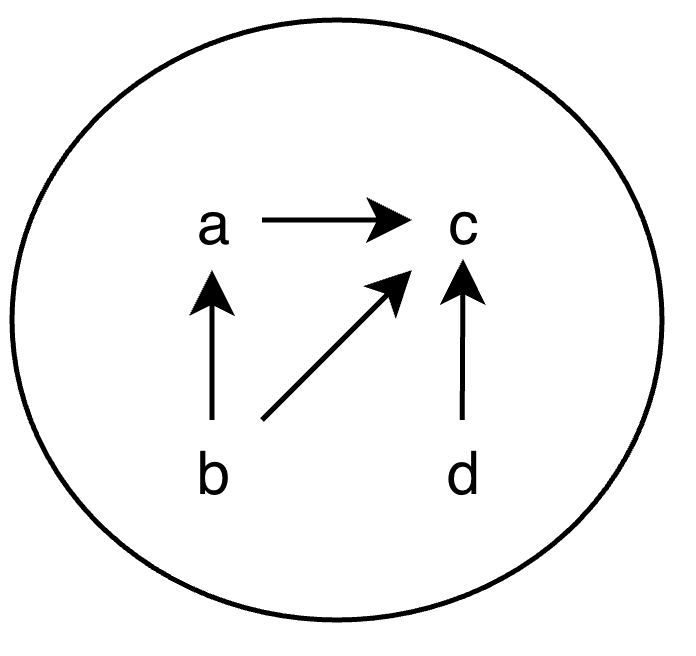
\includegraphics[width=3cm]{images/relazione-transitiva.png}
        \caption{Relazione transitiva}
        \label{fig:relazione-transitiva}
    \end{subfigure}
    \hspace{1.5cm}
    \begin{subfigure}{.3\textwidth}
        \centering
        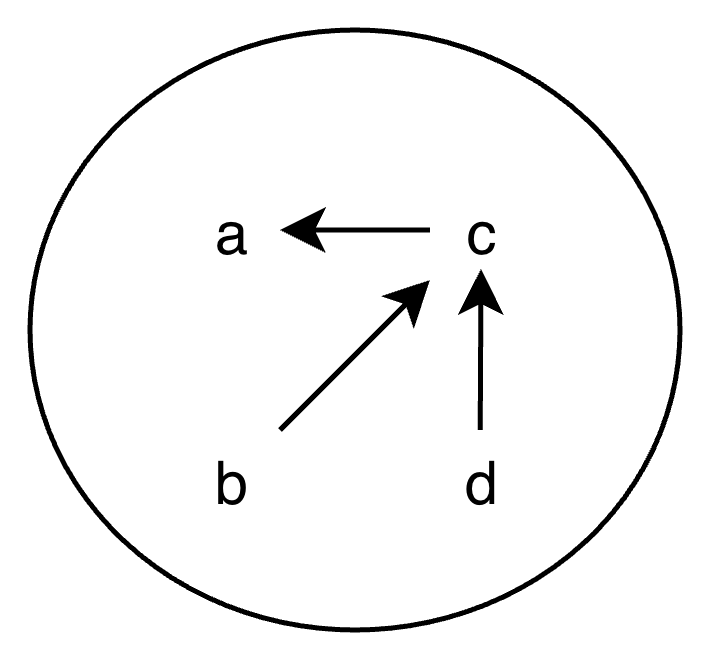
\includegraphics[width=3cm]{images/relazione-non-transitiva.png}
        \caption{Relazione non transitiva}
        \label{fig:relazione-non-transitiva}
    \end{subfigure}
\end{figure}
\newpage
\begin{example}
Alcuni esempi di relazioni transitiva:
    \begin{itemize}
        \item L'Identità di A $Id_A: A \longleftrightarrow A$ è transitiva.
        \item La relazione completa $A$ X $A:A \longleftrightarrow A$ è transitiva.
        \item La relazione vuota $\O: A \longleftrightarrow A$ è transitiva.
        \item La relazione minore $<: \mathbb{N} \longleftrightarrow \mathbb{N}$ è transitiva.
        \item La relazione minore-uguale $\leq: \mathbb{N} \longleftrightarrow \mathbb{N}$ è transitiva.
        \item La relazioni di amicizia su facebook FbFreind: FB $\longleftrightarrow$ FB non è transitiva perché se te sei amico di una persona e questa persona ha amico un altro utente non necessariamente te sei amico di quest'altro utente.
        \item La relazioni di follow su instagram IGFollow: IG $\longleftrightarrow$ IG non è transitiva perché se te hai come follow una persona e questa persona ha come follow un altro utente non necessariamente te sei hai come follow di quest'altro utente.
    \end{itemize}
\end{example}

\subsubsection{Anti-simmetrica}
Dato un inseme A, una relazione $R: A \longleftrightarrow A$ possiamo definirla come:
\begin{definition}[Anti-simmetrica]
    R è una relazione \textbf{Anti-simmetrica} se per tutti gli $a,b \in A$ vale che se $(a, b) \in R$ e $(b, a) \in R$ allora $a = b$
    \begin{center}
        $\forall \: a,b \in A . (a, b) \in R \land (b, a) \in R \Longrightarrow a = b$
    \end{center}
\end{definition}
Rappresentiamo \textbf{graficamente} ora una relazione anti-simmetrica. \\Dato un insieme A di partenza dove A = $\{a, b, c, d\}$:
\begin{itemize}
    \item Il caso [\ref{fig:relazione-anti-simmetrica}] è anti-simmetrica perché la premessa è negata, quindi per le varie coppie di valori non esistono coppie simmetriche.
    \item Il caso [\ref{fig:relazione-non-anti-simmetrica}] non è anti-simmetrica perché esiste sia la coppia (a,b) e (b,a) ma a è diverso da b.
\end{itemize}
\begin{figure}[h!]
    \vspace{-10pt}
    \centering
    \begin{subfigure}{.3\textwidth}
        \centering
        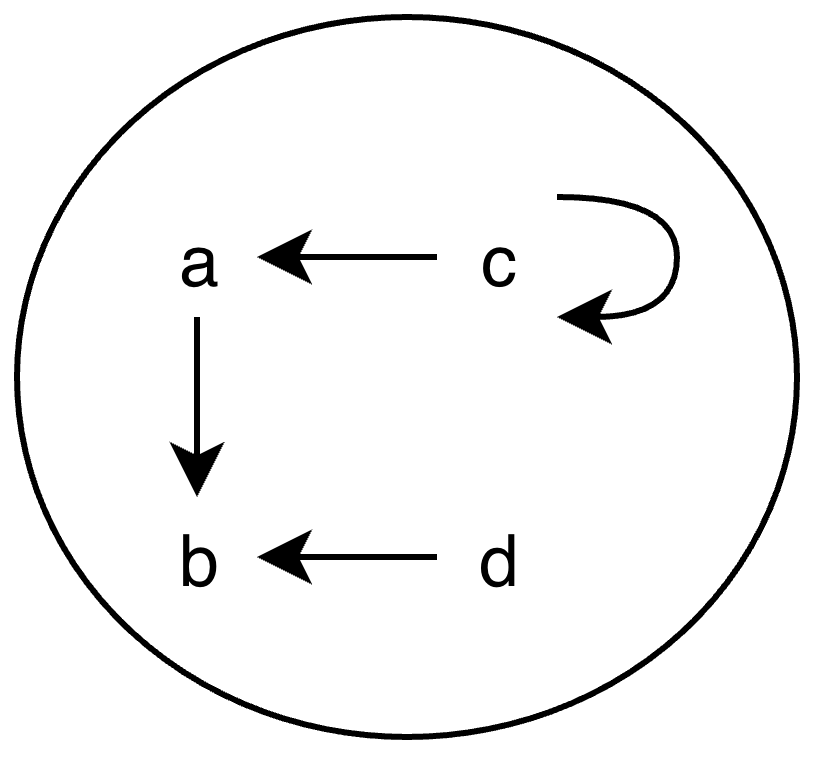
\includegraphics[width=3cm]{images/relazione-anti-simmetrica.png}
        \caption{Relazione anti-simmetrica}
        \label{fig:relazione-anti-simmetrica}
    \end{subfigure}
    \hspace{1.5cm}
    \begin{subfigure}{.3\textwidth}
        \centering
        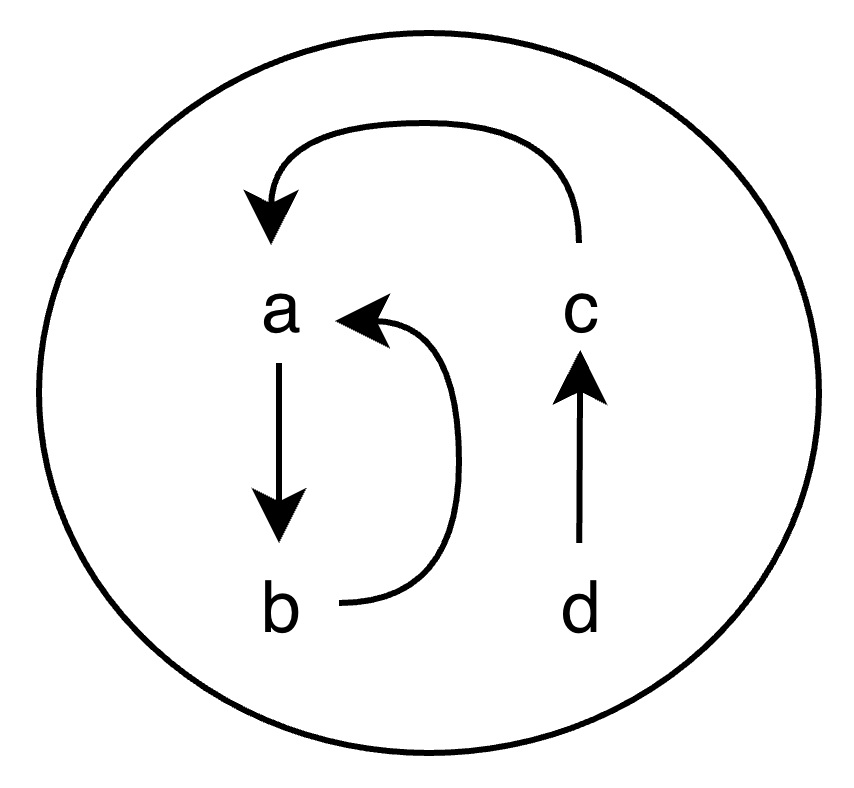
\includegraphics[width=3cm]{images/relazione-non-anti-simmetrica.png}
        \caption{Rel. non anti-simmetrica}
        \label{fig:relazione-non-anti-simmetrica}
    \end{subfigure}
\end{figure}
\begin{example}
Alcuni esempi di relazioni anti-simmetrica:
    \begin{itemize}
        \item L'Identità di A $Id_A: A \longleftrightarrow A$ è anti-simmetrica.
        \item La relazione completa $A$ X $A:A \longleftrightarrow A$ non è anti-simmetrica perchè sicuramente esisterà sia (a,b) che (b,a) ma non necessariamente a = b.
        \item La relazione vuota $\O: A \longleftrightarrow A$ è anti-simmetrica.
        \item La relazione minore $<: \mathbb{N} \longleftrightarrow \mathbb{N}$ è anti-simmetrica \footnote{Ricorda che se cade la premessa allora la conclusione è sempre vera per le leggi logiche sugli operatori}.
        \item La relazione minore-uguale $\leq: \mathbb{N} \longleftrightarrow \mathbb{N}$ è anti-simmetrica.
    \end{itemize}
\end{example}

\subsection{Teorema di caratterizzazione}
\begin{theorem}[Teorema di caratterizzazione]\label{Teorema-caratterizzazione}
    Pero tutti gli insiemi A e per tutte le relazioni $R: A \longleftrightarrow A$ vale che:
    \begin{enumerate}
        \item R è \textbf{riflessiva} $\Longleftrightarrow$ $Id_A \subseteq R$.
        \item R è \textbf{simmetrica} $\Longleftrightarrow$ $R \subseteq R^{op}$ (o anche $R^{op} \subseteq R, R = R^{op}$).
        \item R è \textbf{transitiva} $\Longleftrightarrow$ $R;R \subseteq R$.
        \item R è \textbf{anti-simmetrica} $\Longleftrightarrow$ $R \cap R^{op} \subseteq Id_A$.
    \end{enumerate}
\end{theorem}
\begin{demostration}[Simmetrica]
Proviamo a dimostrare il punto 2 quindi che R è \textbf{simmetrica} $\Longleftrightarrow$ $R \subseteq R^{op}$ (o anche $R^{op} \subseteq R, R = R^{op}$).\\\\
Per effettuare questa dimostrazione andiamo a dimostrare i due sensi dell'implicazione (in due sensi della freccia $\Longleftrightarrow$).
\begin{itemize}
    \item $\forall \: (a,b) \in R \Longrightarrow (b,a) \in R \Longrightarrow R \subseteq R^{op}$.\\
    Noi sappiamo che per la proprietà simmetrica che per ogni coppia di valori (a,b) dovrà esistere (b,a), quindi l'insieme R sarà composto da una serie di coppie e i loro opposti. Da qui deduciamo come se $(b,a) \in R$ e $(a,b) \in R$ e l'opposto di R, $R^{op}$, conterrà ugualmente tutte le coppie di R soltanto invertite (per la definizione di opposto), farà si che, essendo già presenti le coppie di valori invertite in R, $R \subseteq R^{op}$. In maniera più formale:
    $\forall (a,b) \in R$ sarà presente un $\forall (a,b) \in R^{op}$ e $\forall (b,a) \in R$ sarà presente un $\forall (b,a) \in R^{op}$ per la definizione di op e di simmetria.
    \item $R \subseteq R^{op} \Longrightarrow \forall \: (a,b) \in R \Longrightarrow (b,a) \in R $.\\
    Per dimostrare la proprietà simmetrica partendo da $R \subseteq R^{op}$ consideriamo che: $(a,b) \in R$ per assunzione $(a,b) \in R^{op}$ ma per definizione di opposto, per far in modo che $(a,b) \in R$ allora $(b,a) \in R$, è così dimostrato anche questo senso dell'implicazione.
 \end{itemize}
\end{demostration}

\subsection{Chiusure}
Le chiusure servono per rendere una relazione in un determinato modo tra riflessiva, simmetrica transitiva, applicando delle operazioni fra insiemi.
\subsubsection{Chiusura riflessiva}
La chiusura riflessiva di R è il modo "minimale" per rendere R riflessiva.
\begin{definition}[Chiusura riflessiva]
    Sia $R: A \longleftrightarrow A$ una relazione su in insieme A, la chiusura \textbf{riflessiva} di R è la relazione $R \cup Id_A$
\end{definition}
\begin{example}
Alcuni esempi di chiusure riflessive:\\
$Id_A: A \longleftrightarrow A$ = $Id_A$ \hspace{.7cm} $A: A \longleftrightarrow A$ = $A$ X $A$ \hspace{.7cm} $\O: A \longleftrightarrow A$ = $Id_A$ \\$<: \mathbb{N} \longleftrightarrow \mathbb{N}$ = $\leq$  \hspace{.7cm} $\leq: \mathbb{N} \longleftrightarrow \mathbb{N}$ = $\leq$
\end{example}
\begin{note}
Nota che per ogni $S: A \longleftrightarrow A$, se $R \subseteq S$ ed $R$ è riflessiva, allora $R \cup Id_A \subseteq S$ 
\end{note}

\subsubsection{Chiusura simmetrica}
La chiusura simmetria di R è un metodo "minimale" per rendere R simmetrica.
Sia $R: A \longleftrightarrow A$ una relazione su in insieme A:
\begin{definition}[Chiusura simmetrica]
    Sia $R: A \longleftrightarrow A$ una relazione su in insieme A, la chiusura \textbf{simmetrica} di R è la relazione $R \cup R^{op}$
\end{definition}
\begin{example}
Alcuni esempi di chiusure riflessive:\\
$Id_A: A \longleftrightarrow A$ = $Id_A$ \hspace{.7cm} $A: A \longleftrightarrow A$ = $A$ X $A$ \hspace{.7cm} $\O: A \longleftrightarrow A$ = $\O$ \\$<: \mathbb{N} \longleftrightarrow \mathbb{N}$ = $\neq$  \hspace{.7cm} $\leq: \mathbb{N} \longleftrightarrow \mathbb{N}$ = $\mathbb{N}$ X $\mathbb{N}$
\end{example}

\begin{note}
Nota che per ogni $S: A \longleftrightarrow A$, se $R \subseteq S$ ed $R$ è simmetria, allora $R \cup R^{op} \subseteq S$ 
\end{note}

\subsubsection{Chiusura transitiva}
Per arrivare a capire la chiusura transitiva come opera bisogna partire da un'intuizione. La proprietà transitiva intanto dice in maniera informale che $\forall x,y \in A X A. \exists (x,y)$ se $x$ "può raggiungere" $y$ in R; capiamo dunque come la chiusura transitiva arricchisce R con tutte le coppie (x,y) tali che y è raggiungibile da x seguendo degli archi.\\ \\
Sia data dunque una relazione $R: A \longleftrightarrow A$ dove $R = \{(a,b), (b,c), (c,d), (d,e), (d,f)\}$, e rappresentiamo graficamente i vari "passaggi per rendere tale relazione transitiva.
\begin{figure}[h!]
    \centering
    \begin{subfigure}{.3\textwidth}
        \centering
        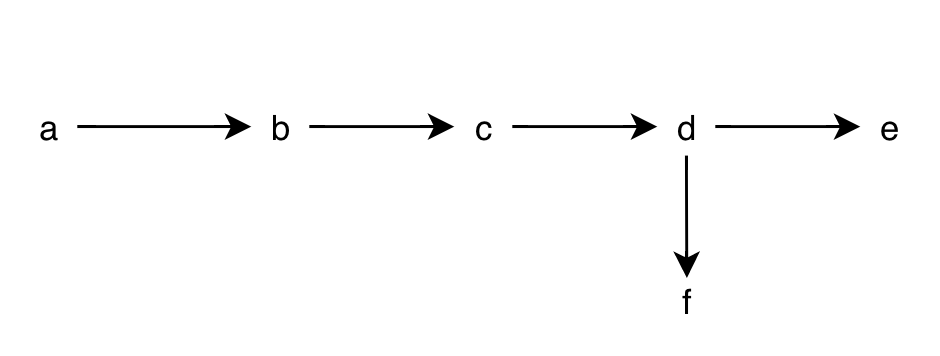
\includegraphics[width=5cm]{images/chiusura-transitiva-1.png}
        \caption{R}
        \label{}
    \end{subfigure}
    \hfill
    \begin{subfigure}{.3\textwidth}
        \centering
        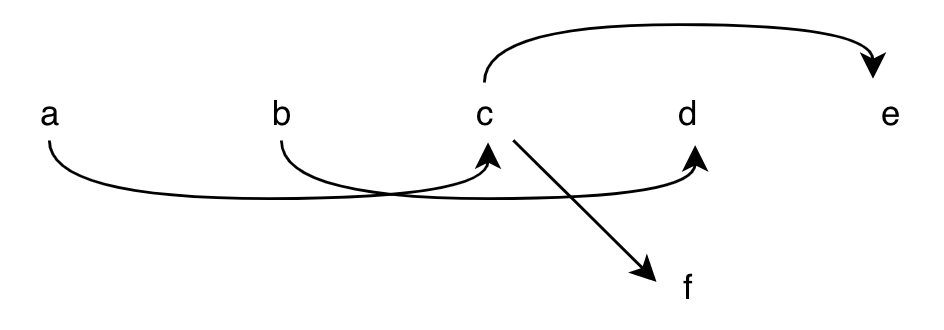
\includegraphics[width=5cm]{images/chiusura-transitiva-2.png}
        \caption{R;R}
        \label{}
    \end{subfigure}
    \hfill
    \begin{subfigure}{.3\textwidth}
        \centering
        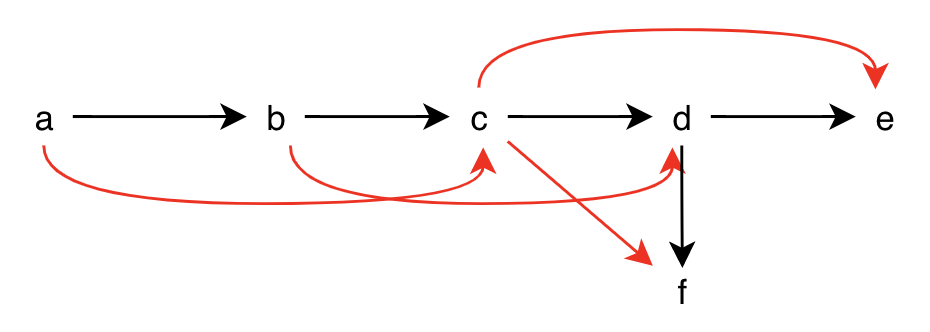
\includegraphics[width=5cm]{images/chiusura-transitiva-3.png}
        \caption{R $\cup$ R;R}
        \label{}
    \end{subfigure}
    \hfill
    \begin{subfigure}{.3\textwidth}
        \vspace{15pt}
        \centering
        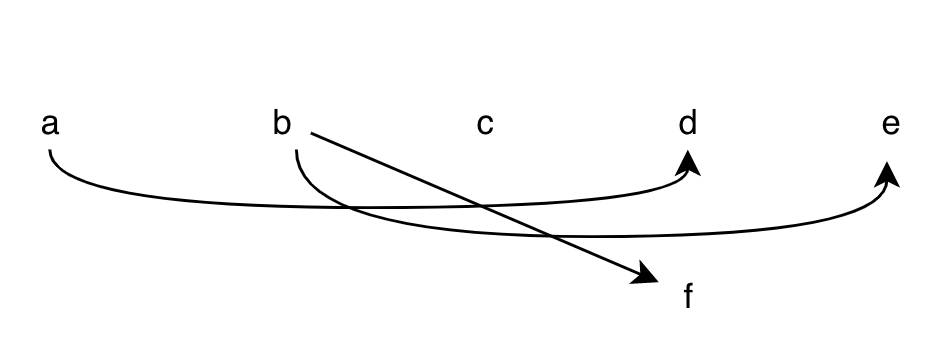
\includegraphics[width=5cm]{images/chiusura-transitiva-4.png}
        \caption{(R;R);R}
        \label{}
    \end{subfigure}
    \hfill
    \begin{subfigure}{.3\textwidth}
        \vspace{15pt}
        \centering
        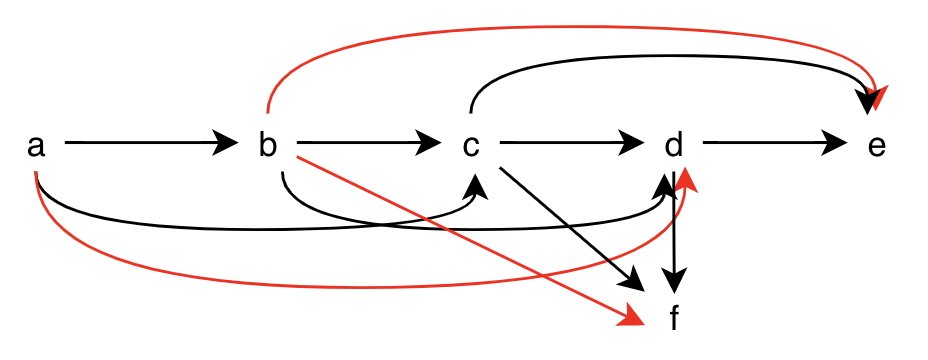
\includegraphics[width=5cm]{images/chiusura-transitiva-5.png}
        \caption{R $\cup$ R;R $\cup$ R;R;R}
        \label{}
    \end{subfigure}
    \hfill
    \begin{subfigure}{.3\textwidth}
        \vspace{15pt}
        \centering
        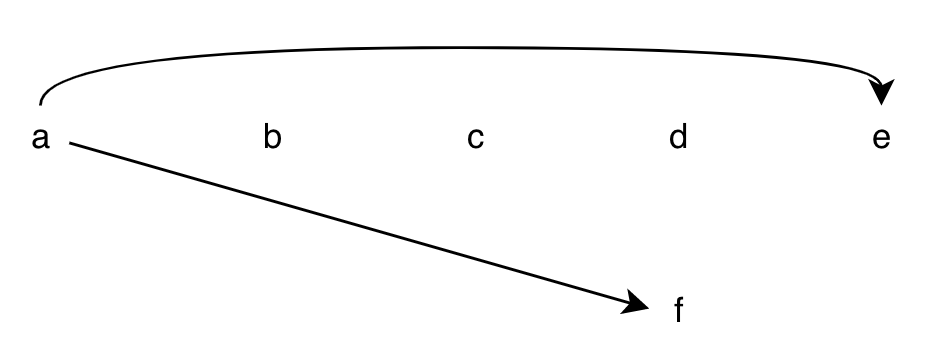
\includegraphics[width=5cm]{images/chiusura-transitiva-6.png}
        \caption{((R;R);R);R}
        \label{}
    \end{subfigure}
    \hfill
    \begin{subfigure}{.3\textwidth}
        \vspace{15pt}
        \centering
        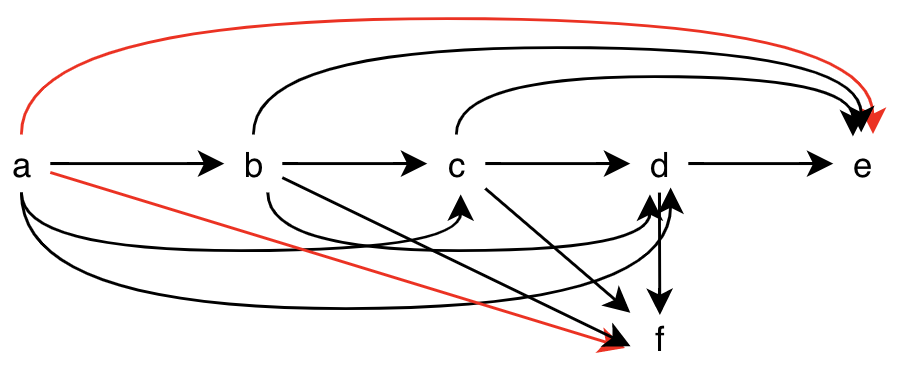
\includegraphics[width=5cm]{images/chiusura-transitiva-7.png}
        \caption{R $\cup$ R;R $\cup$ R;R;R $\cup$ R;R;R;R}
        \label{}
    \end{subfigure}
    \hspace{2cm}
    \begin{subfigure}{.3\textwidth}
        \vspace{15pt}
        \centering
        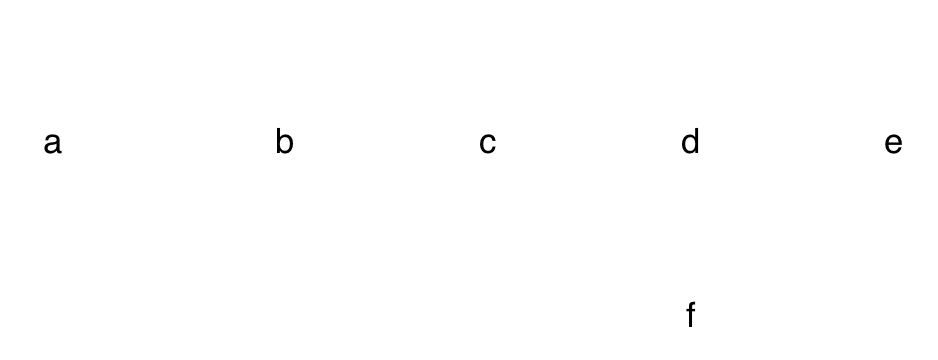
\includegraphics[width=5cm]{images/chiusura-transitiva-8.png}
        \caption{(((R;R);R);R);R}
        \label{}
    \end{subfigure}
\end{figure}
\\
Come si vede nelle sequenza di passi sopra, il metodo per fra diventare una relazione transitiva si basa sul ripetere una serie di composizioni ed unirle fra loro finché non si raggiunge uno stato o di vuoto (come in questo caso) o di loop. Questo genere di operazione può essere definita in modo più formale tramite la composizione n-aria di relazione.
\begin{definition}[Composizione n-aria di relazione]
    Sia A u insieme e $R: A \longleftrightarrow A$ una relazione su A, $\forall n \in \mathbb{N}$, la composizione n-aria della relazione R, $R^n$ è definita induttivamente come:
    \begin{enumerate}
        \item \underline{Caso base:} $R^0 = Id_A$
        \item \underline{Passo induttivo:} $R^{n+1} = R;R^n$
    \end{enumerate}
\end{definition}
\begin{example}
$R^0 = Id_A$ \hspace{.3cm} $R^1 = R;Id_A = R$ \hspace{.3cm} $R^2 = R;R$ \hspace{.3cm} $R^3 = R;R;R$ e così via.
\end{example}
Ora possiamo chiaramente definire la chiusura transitiva.
\begin{definition}[Chiusura transitiva]
    Sia $R: A \longleftrightarrow A$ una relazione su in insieme A, la chiusura transitiva di R è la relazione definita come $R^{+} = \bigcup\limits_{n \in \mathbb{N}^+} R^{n}$ con $\O \notin R^{+}$.
\end{definition}
\begin{example}
Alcuni esempi di chiusure transitiva:\\
$Id_A^+ = Id_A$ \hspace{.7cm} $(A: A \longleftrightarrow A)^+$ = $A$ X $A$ \hspace{.7cm} $(\O: A \longleftrightarrow A)^+$ = $\O$
\end{example}

\subsection{Stella di kleene}
\begin{definition}[Stella di kleene]
    Sia A un insieme ed $R: A \longleftrightarrow A$ una relazione su A. La chiusura di kleene (o stella di kleene) è la combinazione della chiusura riflessiva e transitiva di R ed è definita come:
    \begin{center}
         $R^* = \bigcup\limits_{n \in \mathbb{N}} R^n$ \:\: quindi \:\: $R^* = (R^+) \cup (Id_A)$
    \end{center}
\end{definition}
\begin{example}
Facciamo un esempio in cui consideriamo l'insieme $A = \{a,b,c,d\}$ ed applichiamo la stella di kleene alla relazione $R = \{(a,b),(a,d),(b,c)\}$.
\end{example}
\begin{figure}[h!]
    \vspace{-20pt}
    \begin{subfigure}{.3\textwidth}
        \centering
        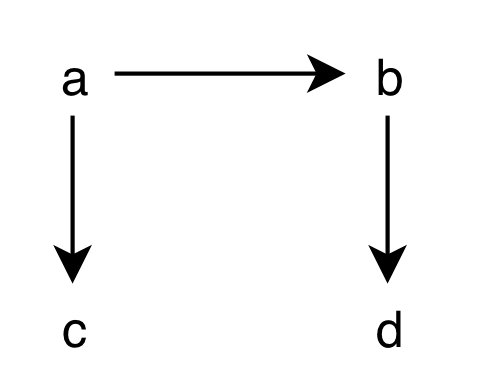
\includegraphics[width=4cm]{images/stella-kleene-1.png}
        \caption{R di partenza}
    \end{subfigure}
    \hfill
    \begin{subfigure}{.3\textwidth}
        \centering
        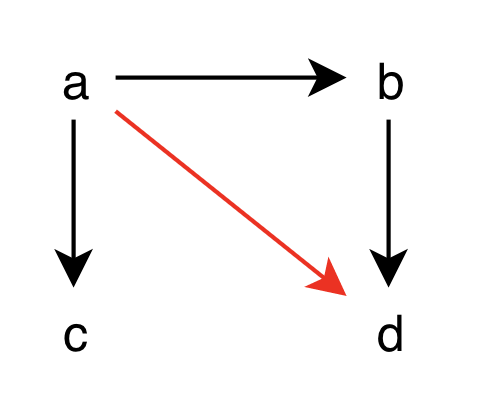
\includegraphics[width=4cm]{images/stella-kleene-2.png}
        \caption{R di partenza + transitiva (rosso)}
    \end{subfigure}
    \hfill
    \begin{subfigure}{.3\textwidth}
        \centering
        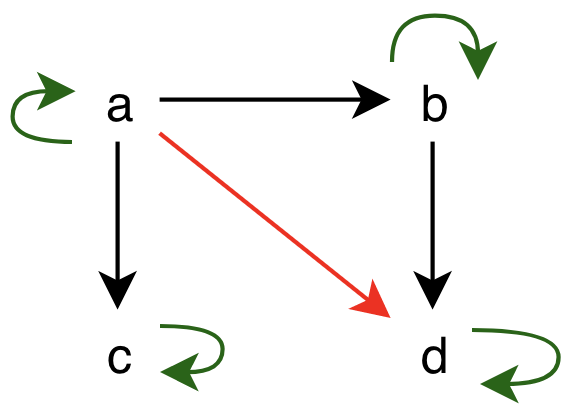
\includegraphics[width=4cm]{images/stella-kleene-3.png}
        \caption{R di partenza + transitiva (rosso) + riflessiva (verde)}
    \end{subfigure}
\end{figure}

\subsubsection{Apllicazione al While}
Prendiamo come esempio questo pezzo di codice while:
\begin{center}
    while ($x \geq 2$) do $\{x = x - 2\}$
\end{center}
Andiamo ora a definire i 3 componenti di questo ciclo.
\begin{itemize}
    \item $C = \{(x, x-2) | x \in \mathbb{Z}\}: \mathbb{Z} \longleftrightarrow \mathbb{Z}$.
    Identifica il \textbf{corpo} del while, cioè $x = x - 2$, che è la parte che viene eseguita ad ogni iterazione.
    \item $G = \{(x,x) | x \in \mathbb{Z} \: \land \: x \geq 2\}: \mathbb{Z} \longleftrightarrow \mathbb{Z}$. Identifica la \textbf{guardi}, cioè $x \geq 2$. Si può notare che $G \subseteq Id_{\mathbb{Z}}$ essendo che associa coppie di valori uguali, l'unica cosa che contraddistingue $G$ dall'identità e che i valori devono soddisfare la condizione $x \geq 2$.
    \item $\overline{G} = \{(x,x)\:|\:x \in \mathbb{Z} \: \land \: x < 2\}$.
    Identifica la \textbf{negazione della guardia} che sarebbe $\overline{G} = Id_{\mathbb{Z}} \setminus G$ cioè tutti i valori che non rispettano la condizione del while.
\end{itemize}
Utilizziamo i 3 componenti appena scritti per andare a definire il pezzo di programma sopra come una relazione.
\begin{equation}\label{while-relazione}
    W = (G;C)^*;\overline{G}
\end{equation}
Spieghiamo velocemente la forma scritta sopra [\ref{while-relazione}]. L'obbiettivo è ottenere una relazione che associ un valore consentito dalla guardia al valore finale che uscirà dal while.\\
La prima composizione che troviamo (G;C) è una relazione che dato una qualsiasi numero che rispetti le regole scritte nella guardia restituisce quel numero meno 2 ($x = x - 2$); andando poi ad applicare la stella di kleene su quella relazione, $(G;C)^*$ stiamo semplicemente aggiungendo la proprietà transitiva e riflessiva all'insieme, quindi per qualsiasi numero che rispetta le condizioni della guardia esisteranno delle coppie per tutti i "cicli" che il while permette, facciamo un esempio: prendiamo $x = 6$, il valore di x rispetta la guardia perché $x \in \mathbb{Z}$ e $x \geq 2$, inoltre, per la prima composizione, esisterà anche la coppia $(x, x-2)$ e cioè (6,4); ora, visto che la relazione è composta da tutti i numeri appartenenti a $\mathbb{Z}$ esisterà anche la coppia con partenza $x = 4$ e quindi formata da (4,2) e così anche le coppie (2,2) e (2,0); se applichiamo quindi la proprietà transitiva si andranno allora a creare le coppie (6,4), (6,2) e (6,0) che possiamo vedere che sono i vari passaggi del while.\\
Arrivati a questo punto però noi vogliamo ottenere una relazione che dano un valore restituisca il risultato finale del ciclo, quindi, riferendosi all'esempio di prima, basterà "eliminare" tutte le coppie "intermedie, e questo si fa con l'ultima composizione, $(G;C)^*;\overline{G}$ dove $;\overline{G}$ permette di creare coppie fra i valori di partenza e il valore che non rispetta più la condizione del while, quindi (6,0), (4,0) ecc.
\begin{demostration}
    Andiamo ora a dimostrare che per ogni coppia $(a,b) \in \mathbb{Z}$ X $\mathbb{X}$, $(a,b) \in W$ se e solo se il programma while eseguito a partite da uno stato in cui $x = a$ termina in uno stato in cui $x = b$. \\ \\
    \textbf{Caso 1°} (\underline{$x < 2$}) - Quello che dobbiamo dimostrare in questo caso è che le coppie $(a,a) \in W$ perché dati dei valori inferiori a 2 il ciclo non parte e quindi restituirà lo stesso valore.\\ \\ In questo caso teoricamente per la legge con cui è costruita la relazione G, $(a,a) \neq G$ e per cioè si verifica anche la condizione $(a,a)\neq G;C$, però nel caso $(G;C)^*$ si aggiunge all'insieme anche tutta $Id_{\mathbb{Z}}$ per la proprietà della stella di kleene, $Id_{\mathbb{Z}} \subseteq (G;C)^*$, allora arriviamo a vedere che $(a,a) \in (G;C)^*$ e che $(a,a) \in \overline{G}$ (questo perché a sono i valori minori di 2 e quindi rispettano la legge della relazione $\overline{G}$) quindi di conseguenza $(a,a) \in (G;C)^*;\overline{G}$ come desiderato. $\blacksquare$ \\ \\
    \textbf{Caso 2°} (\underline{$x \geq 2$}) - In questo caso dobbiamo invece dimostrare l'appartenenza all'insieme W di tutte le coppie con un x di partenza valido per l'attivazione del ciclo while.\\ \\
    Questa seconda casistica si dimostra in maniera intuitiva. Vediamo come prima cosa che $(a,a) \in G$ e $(a,a-2) \in C$ quindi $(a,a-2) \in (G;C)$, quindi per ogni $a \geq 2$ si andranno a costruire i vari passaggi del while, descrivibile come $(G;C)^n$ con $n \in \mathbb{N}^+$ dove $n$ è l'n-esima iterazione. Ad esempio:
    \begin{table}[h!]
        \centering
        \begin{tabular}{c c}
            $(6,4) \: \: \in \: \: (G;C)^1$ & $(7,5) \: \: \in \: \: (G;C)^1$  \\
            $(6,2) \: \: \in \: \: (G;C)^2$ & $(7,3) \: \: \in \: \: (G;C)^2$  \\
            $(6,0) \: \: \in \: \: (G;C)^3$ & $(7,1) \: \: \in \: \: (G;C)^3$ 
        \end{tabular}
    \end{table}
    \begin{note}
    \vspace{-10pt}
    Nota che nell'esempio sopra $(6, -2) \notin (G;C)^4$ in quanto $(0, -2) \notin G;C$
    \end{note}
    Ora per concludere la dimostrazione basta considerare che la composizione $(G;C)^*;\overline{G}$ va ad associare ogni interazione valida all'interno di while $(a,a-2)$ con i valori che non la validano (che si trovano nella relazione $\overline{G}$) quindi seguendo l'esempio sopra $(7,1) \in W$ e $(6,0) \in W$. Poiché questo ragionamento può essere applicato ag ogni numero pari o dispari maggiore o uguale a 2, questo conclude anche questo caso della dimostrazione. $\blacksquare$
\end{demostration}

\subsubsection{Leggi stella di kleene}
Per tutti gli insiemi A e le relazioni $R: A \longleftrightarrow A$ e $S: A \longleftrightarrow A$ valgono le seguenti uguaglianze.
\begin{table}[h!]
    \centering
    \setlength{\tabcolsep}{10pt}
    \renewcommand{\arraystretch}{1.3}
    \begin{tabular}{|c|c|}
        \hline
        \textbf{Riflessività} & $Id_A \subseteq R^*$ \\
        \textbf{Transitività} & $R^*;R^* \subseteq R^*$ \\
        \textbf{Chiusura} & $R \subseteq R^*$ \\
        \textbf{Indempotenza} & $(R^*)^* = R^*$ \\
        \textbf{*-id} & $Id_A^* = Id_A$ \\
        \textbf{*-compl} & $(A$ X $A)^*$ = $A$ X $A$  \\
        \textbf{*-vuoto} & $\O_{A;A}^* = Id_A$ \\
        \textbf{Distributività di * su $\cup$} & $R^* \cup S^* \subseteq (R \cup S)^*$ \\
        \textbf{Distributività di * su $\cap$} & $(R \cap S)^* \subseteq R^* \cap S^*$ \\
        \textbf{Distributività di * su $.^{op}$} & $(R^*)^{op} = (R^{op})^*$ \\
        \hline
    \end{tabular}
    \caption{Leggi stella di Kleene}
    \label{tab:leggi-stella-kleene}
\end{table}

\subsection{Relazioni di equivalenza}
\begin{definition}[Relazioni di equivalenza]
    Sia A un insieme $R: A \longleftrightarrow A$ una relazione su A, si dice che R è una relazione di equivalenza se \textbf{riflessiva}, \textbf{simmetrica}, \textbf{transitiva}. 
\end{definition}
\begin{example}
Alcuni esempi di relazioni di equivalenza:\\
$Id_A: A \longleftrightarrow A$ SI \hspace{.7cm} $A: A \longleftrightarrow A$ SI \hspace{.7cm} $\O: A \longleftrightarrow A$ NO \\$<: \mathbb{N} \longleftrightarrow \mathbb{N}$ NO perché non riflessiva \hspace{.7cm} $\leq: \mathbb{N} \longleftrightarrow \mathbb{N}$ NO perché non simmetrica
\end{example}

\subsubsection{Classe di equivalenza}
\begin{definition}[Classe di equivalenza]
    Data $R: A \longleftrightarrow A$ una relazione di equivalenza, ed $a \in A$, la classe di equivalenza di a si definisce come l'insieme: 
    \begin{equation}
        [a]_R = \{b \in A \:|\: (a,b) \in R\}
    \end{equation}
\end{definition}
La definizione vuol dire che, una classe di equivalenza di un determinato insieme di relazioni è un insieme di elementi appartenenti a questa relazione il quale, questi elementi, sono legati fra di loro da una relazione.
\begin{example}
    Prendiamo $A = \{a,b,c,d\}$ ed $R = \{(a,b), (b,a), (a,a), (b,b), (c,c), (d,d)\}$\\
    Le classi di equivalenza saranno per ogni elemento di A le seguenti:\\
    $[a]_R = \{a,b\}$ \hspace{.5cm} $[b]_R = \{a,b\}$ \hspace{.5cm} $[c]_R = \{c\}$ \hspace{.5cm} $[d]_R = \{d\}$
\end{example}
\begin{example}
    Altri esempi di classi di equivalenza. Dato un insieme A si considerino le relazioni $Id_A$ e la relazione $A$ X $A$, per tutti gli $a \in A$ vale che: \: \: \:
    $[a]_{Id_A} \: = \: \{a\}$ \hspace{.7cm} $[a]_{A \times A} \: = \: A$
\end{example}

\subsubsection{Teorema di biiezione}
\begin{definition}[Partizione]
    Dato un $F = A_1, A_2, A_3, ..., A_k$, F è una partizione di A se:
\end{definition}
\begin{enumerate}
    \item $\forall i \: A_i \neq \O$
    \item $\bigcup^m_{i=1}A_j = A$
    \item $\forall i, j A_i \cap A_j = \O\text{ con } i \neq j$
\end{enumerate}
Ora con la definizione di partizione e di classe di equivalenza possiamo osservare che:
\begin{itemize}
    \item L'insieme di tutte le classi di equivalenza di R definisce una partizione dell'insieme A.
    \[EC_R = \{[a]_r \:|\: a \in A\}\]
    \item Viceversa, ogni partizione di A definisce una relazione di equivalenza.
    \begin{center}
        $Rf = \{(a,b) \in A \times A \: | \: \exists i a,b \in A_i\}$
    \end{center}
\end{itemize}

\begin{theorem}[Teorema di biiezione]
    Sia A un insieme, ERel(A) l'insieme di tutte le relazioni di equivalenza su A, Part(A) l'insieme di tutte le partizioni su A. Allora:
    \begin{equation}
        ERel(A) \cong Part(A)
    \end{equation}
\end{theorem}

\subsection{Relazioni di ordinamento}
\subsubsection{Ordinamento parziale}
\begin{definition}[Ordinamento parziale]
    Sia A un insieme e $R: A \longleftrightarrow A$ una relazione su A. Si dice che R è una relazione di ordinamento parziale se è \textbf{riflessiva}, \textbf{transitiva} e \textbf{anti-simmetrica}.
\end{definition}
\begin{note}
    Nota che gli ordinamenti si scrivono utilizzando o il simbolo $\prec$, $\preceq$ oppure $\sqsubset$, $\sqsubseteq$.
\end{note}
\begin{example}
Alcuni esempi di ordinamento parziale:\\
$Id_A: A \longleftrightarrow A$ SI \hspace{.7cm} $A: A \longleftrightarrow A$ NO  \hspace{.7cm} $\O: A \longleftrightarrow A$ NO \\$<: \mathbb{N} \longleftrightarrow \mathbb{N}$ NO perché non riflessiva \hspace{.7cm} $\leq: \mathbb{N} \longleftrightarrow \mathbb{N}$ SI.
\end{example}

\begin{proposition}
Per ogni insieme A, l'inclusione $\mathcal{P}(X)$ è una relazione di ordinamento parziale, e si scrive come:
\begin{center}
    $\{(X,Y) \in \mathcal{P}(X) \times \mathcal{P}(X) \: | \: X \subseteq Y\}$
\end{center}
\end{proposition}
Per capire se la proposizione scritta sopra è vera dobbiamo verificare che la relazione create abbia le proprietà riflessiva, transitiva ed anti-simmetrica.\\ \\
Innanzitutto capiamo cosa crea questo insieme. Essendo il prodotto cartesiano fra due insiemi della parti su un insieme A sarà formato da coppie ordinate costituiate da insiemi (essendo che l'insieme $\mathcal{P}(X)$ è un insieme di insiemi che contiene tutti i possibili insiemi creabili con A), non è però un prodotto cartesiano "completo" ma verranno prese solo le coppie di valori che rispettano la legge $X \subseteq Y$ che vuol dire che in una coppia ordinata (A,B) dove A e B sono due insiemi $A \subseteq B$.Ora che abbiamo capito da cos'è costituita questa relazioni verifichiamo le varie proprietà.
\begin{enumerate}
    \item \textbf{Riflessiva}: la relazione sarà riflessiva perché al suo interno esisteranno tutte le coppie $(A,A)$, $(B,B)$, $(C,C)$ visto che un insieme è sempre sotto insieme uguale a se stesso.
    \item \textbf{Transitiva}: la relazione sarà anche transitiva visto che se prendiamo due coppie ordinate $(A,B)$ e $(B,C)$ dove per le regole della relazione $A \subseteq B$ e $B \subseteq C$ esisterà anche $(A,C)$ visto che se $A \subseteq B \subseteq C$ allora $A \subseteq C$.
    \item \textbf{Anti-simmetrica}: in fine la relazione sarà anche anti-simmetrica perché se esistono coppie $(A,B)$ dove $A \leq B$ non potrà mai esiste una coppia $(B,A)$ perché se $A \subseteq B$ e $A \leq B$, l'insieme B avrà obbligatoriamente elementi in più di A (non in meno perché in quel caso A non sarebbe sotto insieme) quindi, per le regole della relazione, non potrà esistere la coppia $(B,A)$ quindi la premessa è falsa e quindi la conseguenza, per le regole dell'implicazione, è vera. Mentre nel caso in cui $A = B$ la condizione di anti-simmetria è valida per sua stessa definizione.
\end{enumerate}

\subsubsection{Ordinamento}
\begin{definition}[Ordinamento]
    Sia $R: A \longleftrightarrow A$ una relazione di ordinamento parziale su un insieme A, si dice che R è ordinamento se R soddisfa le seguenti proprietà (totalità). Per tutti gli $(a,b) \in A \times A$ vale che $(b,a) \in R$ oppure $(b,a) \in R$. Formalmente:
    \begin{equation}
        \forall (a,b) \in A \times A \: | \: (a,b) \in R \lor (b,a) \in R
    \end{equation}
\end{definition}
\begin{example}
Alcuni esempi di ordinamento:\\
$Id_A: A \longleftrightarrow A$ NO \hspace{.5cm} $A: A \longleftrightarrow A$ Non è un ordinamento parziale  \hspace{.5cm} $\leq: \mathbb{N} \longleftrightarrow \mathbb{N}$ SI \\$<: \mathbb{N} \longleftrightarrow \mathbb{N}$ Non è un ord. parziale \hspace{.7cm} $\O: A \longleftrightarrow A$ Non è un ord. parziale.
\end{example}

\subsubsection{Ordinamento lessiografico}
\begin{definition}[Ordinamento lessiografico]
    Dato un ordinamento $\sqsubseteq_A: A \longleftrightarrow A$, \textbf{l'ordinamento lessiografico} è: $a_0a_1... a_n \sqsubseteq_{A^*} b_0b_1...b_m$ se esiste $i \in \mathbb{N}$ tale che:
    \begin{enumerate}
        \item $a_j = b_j$ per tutti i $j < i$
        \item $a_i \sqsubseteq_A b_j$ e $a_i \neq b_j$ oppure $i = n+1$ e $n < m$
    \end{enumerate}
\end{definition}
Questo tipo di ordinamento è usato per le parole nei dizionari o negli elenchi. Si usa se dato un insieme A e un ordinamento $\sqsubseteq_A: A \longleftrightarrow A$(ordinamento sui caratteri), si vuole definire un ordinamento $\sqsubseteq_{A^*}: A^* \longleftrightarrow A^*$(ordinamento sulle stringhe) sull'insieme delle stringhe su A.
Noi conosciamo l'ordinamento dei caratteri (l'afabeto), dato questo possiamo, tramite l'ordinamento lessiografico, ordinare le stringhe.
\begin{example}
Dato un $A = \{a,b,c,...,z\}$ con $a \sqsubseteq_A b \sqsubseteq_A c \sqsubseteq_A ... \sqsubseteq_A z$.\\
Allora tramite l'ordinamento lessiografico $alessandro \sqsubseteq_A anna \sqsubseteq_A annarella \sqsubseteq_A ...$
\end{example}
\newpage
\section{Grafi}
\subsection{Grafo orientato}
\begin{definition}[Grafo orientato]
Un grafo orientato è una relazione $E: V \leftrightarrow V$ su un insieme finito $V$. In un grafo $V$ è l'insieme di nodi o vertici, $E$ è l'insieme di archi o lati. Chiamiamo $G$ (o $G^1$, $G_1$, $G_2$) e scriviamo $G = (V,E)$
\end{definition}
 

\begin{example}\label{esempio-grafo-1}
    Qui di seguito un esempio di un grafo:
\end{example}
 
\hspace{-15pt}Dati i due insiemi $V$ e $E$:\\\\
$V = \{0,1,2,3,4,5\}$ \\
$E = \{(0,0), (0,1), (0,5), (1,3), (1,5), (2,1), (3,4), (3,5), (5,3), (5,4)\}$\\ \\
\begin{wrapfigure}[4]{r}{5cm}
    \vspace{-100pt}
    \centering
    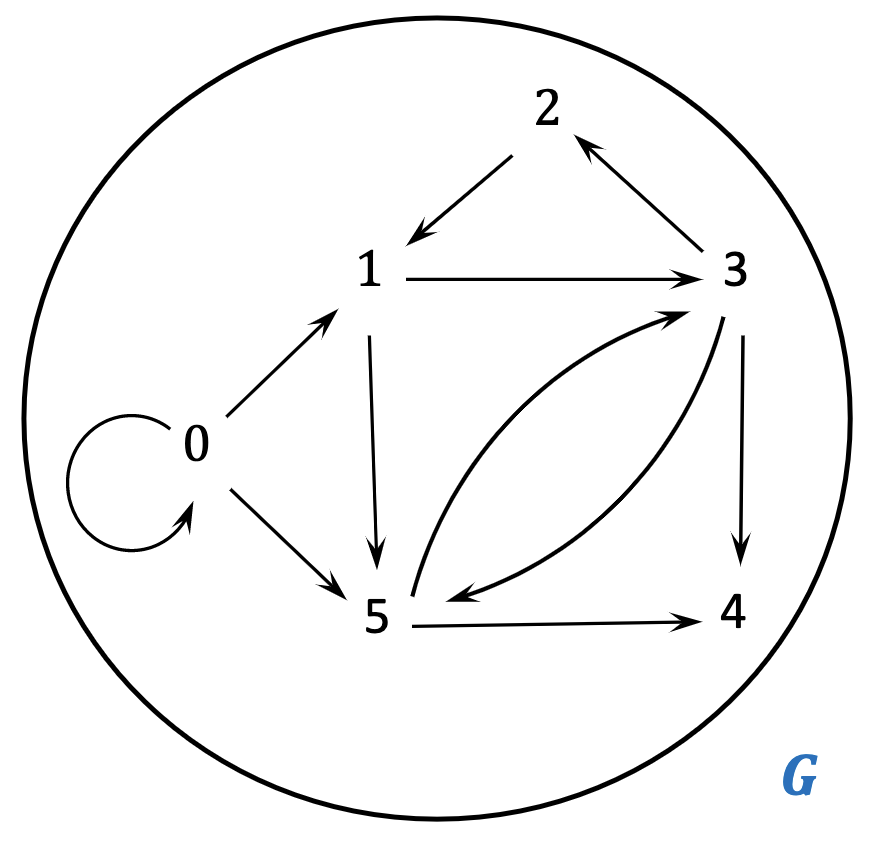
\includegraphics[width=3.7cm]{images/esempio-grafo.png}
    \vspace{-5pt}
    \caption{Grafo G}
    \label{fig:esempio-grafo}
\end{wrapfigure}
Quello rappresentato nell'immagine \ref{fig:esempio-grafo} è un grafo orientato.\\
In questo esempio $n = 6$ e $m = 10$ mentre l'arco $(0,0)$ è un cappio.

\subsubsection{Notazione sui grafi orientati}
Alcune punti di notazione e definizioni sui grafi (Esempi riferiti a immagine \ref{fig:esempio-grafo}):
\begin{itemize}
    \item \textbf{Cardinalità nodi}: $n = \lvert V \rvert $. \hspace{.5cm} \textbf{Cardinalità archi}: $m = \lvert E \rvert$. \hspace{.5cm} $V = \lvert V\rvert = \{0,1,\ldots, \lvert V\rvert-1\}$
    \item \textbf{Cappio}: Un arco $(1,1)$ quindi che parte e ritorna allo stesso nodo lo chiamiamo \textbf{cappio}.
    \item \textbf{Nodi adiacenti}: Nodi $x,y \in V$ sono detti \textbf{adiacenti} se $(x,y) \in E \lor (y,x) \in E$
    \item \textbf{Vicinato in uscita} di $x \in V$: \hspace{.7cm} $N^+(x) = \{y \mid (x,y) \in E\}$.
    \begin{example}
        $N^+(1) = \{3,5\}$.
    \end{example}
    \item \textbf{Vicinato in ingresso} di $x \in V$: \hspace{.7cm} $N^+(x) = \{y \: | \: (y,x) \in E\}$.
    \begin{example}
        $N^-(1) = \{0,2\}$.
    \end{example}
    \item \textbf{Grado di uscita}: dato un nodo $x \in V$: \hspace{.7cm} $d^+_x = |N^+(x)|$.
    \begin{example}
        $d^+_0 = 3$, $d^+_4 = 0$.
    \end{example}
    \item \textbf{Grado di ingresso}: dato un nodo $x \in V$: \hspace{.7cm} $d^-_x = |N^-(x)|$.
    \begin{example}
        $d^+_5 = 3$.
    \end{example}
\end{itemize}

\begin{definition}[Pozzo, sorgente, isolato]
    Definiamo un nodo si dice \textbf{sorgente} se non ha archi entrati, si dice \textbf{pozzo} se non ha archi uscenti e si definisce \textbf{isolato} se non ha ne archi uscenti ne entrati.
\end{definition}

\subsubsection{Grafi orientati come relazioni e proprietà TUSI}
Vediamo ora le quattro proprietà viste per le relazioni (Totale, univalente, surgettiva, iniettiva) come si applicano ai grafi. Dato un grafo orientato $E: V \leftrightarrow V$ possiamo dire che:
\begin{enumerate}
    \item $E: V \leftrightarrow V$ è \textbf{totale} $\Longleftrightarrow$ per ogni nodo $x \in V$ vale $d^+_x \geq 1$.
    \item $E: V \leftrightarrow V$ è \textbf{univalente} $\Longleftrightarrow$ per ogni nodo $x \in V$ vale $d^+_x \leq 1$.
    \item $E: V \leftrightarrow V$ è \textbf{iniettiva} $\Longleftrightarrow$ per ogni nodo $x \in V$ vale $d^-_x \geq 1$.
    \item $E: V \leftrightarrow V$ è \textbf{surgettiva} $\Longleftrightarrow$ per ogni nodo $x \in V$ vale $d^-_x \leq 1$.
\end{enumerate}

\subsubsection{Hand-shaking lemma}
\begin{proposition}[Hand-shaking lemma]
Per ogni grafo orientato $G = (V,E)$, vale che:
\begin{equation}\label{hand-shaking-lemma}
    \sum\limits_{x \in V}d^-_x \: \: \: = \: \: \: \sum\limits_{x \in V}d^+_x \: \: \: = \: \: \: |E|
\end{equation}
\end{proposition}
Questo lemma può essere dimostrando intuitivamente. Se infatti prendiamo un qualsiasi arco fra esso per forza avrà un nodo di partenza ed uno di fine, quindi si dovrà per forza fare un "+1" sia alla somma degli archi entrati, alla somma degli uscenti, che alla somma di tutti gli archi, se questa cosa la estendiamo a tutti gli archi di un grafo possiamo scrivere allora scrivere che $\sum\limits_{x \in V}d^-_x = \sum\limits_{x \in V}d^+_x = |E|$.
\begin{demostration}
Andiamo a dimostrare questa proprietà in modo più formale per induzione:
\begin{enumerate}
    \item \underline{Caso base:} Se $\lvert E\rvert = 0$ non ci sono archi quindi il grado di uscita di ogni nodo sarà per forza 0, e quindi anche la somma di tutti i gradi in uscita sarà 0.
    \begin{center}
        $\sum\limits_{x \in V}d^+_x = 0 = \lvert E\rvert $
    \end{center}
    \item \underline{Passo induttivo:} Supponiamo che la proprietà valga per tutti i grafi con $m$ archi, noi dobbiamo dimostrare il caso $m+1$. \\
    Prendiamo ora un grafo $G = (V,E)$ con $\lvert E\rvert = m+1$, essendo che $\lvert E \rvert > 0$ esiste per forza almeno un arco. Ora rimuoviamo da questo grafo un arco casuale $(i,j) \in E$ tale che si vada a creare un nuovo grafo $G' = (V, E')$ con $E' = E \setminus \{(i,j)\}$, inoltre possiamo anche vedere che in questo nuovo grafo $\lvert E'\rvert = \lvert E\rvert - 1$ che è uguale a $\lvert E'\rvert = m$.\\\\
    Avendo supposto che la proprietà per ogni $m$ sia vera abbiamo che $\sum_{x\in V}d'^+_x = \lvert E'\rvert$. 
    \\Ora noi sappiamo che se escludiamo per esempio $i$ dai nodi abbiamo che $d^+_x = d'^+_x$ per ogni $x \in V \setminus \{ i \}$, mentre $d^+_i = d'^+_i + 1$ perché in $d^+_i$ consideriamo un uscente in più che in $d'^+_i$ non abbiamo e quindi dobbiamo aggiungere. Risulta che quindi se sommiamo i gradi in uscita di $G$ in risultato sarà uguale alla somma dei gradi uscenti di $G'$ + il numero di archi di differenza (in questo caso 1) quindi:
    \begin{center}
        $\sum\limits_{x \in V}d^+_x = \sum\limits_{x \in V}d'^+_x + 1 = \lvert E'\rvert + 1 = \lvert E\rvert $
    \end{center}
    E così dimostrata questa proposizioni tramite induzione. $\blacksquare$
\end{enumerate}
\end{demostration}

\subsection{Rappresentazione grafi}
\begin{figure}[h!]
    \centering
    \begin{subfigure}{.3\textwidth}
        \centering
        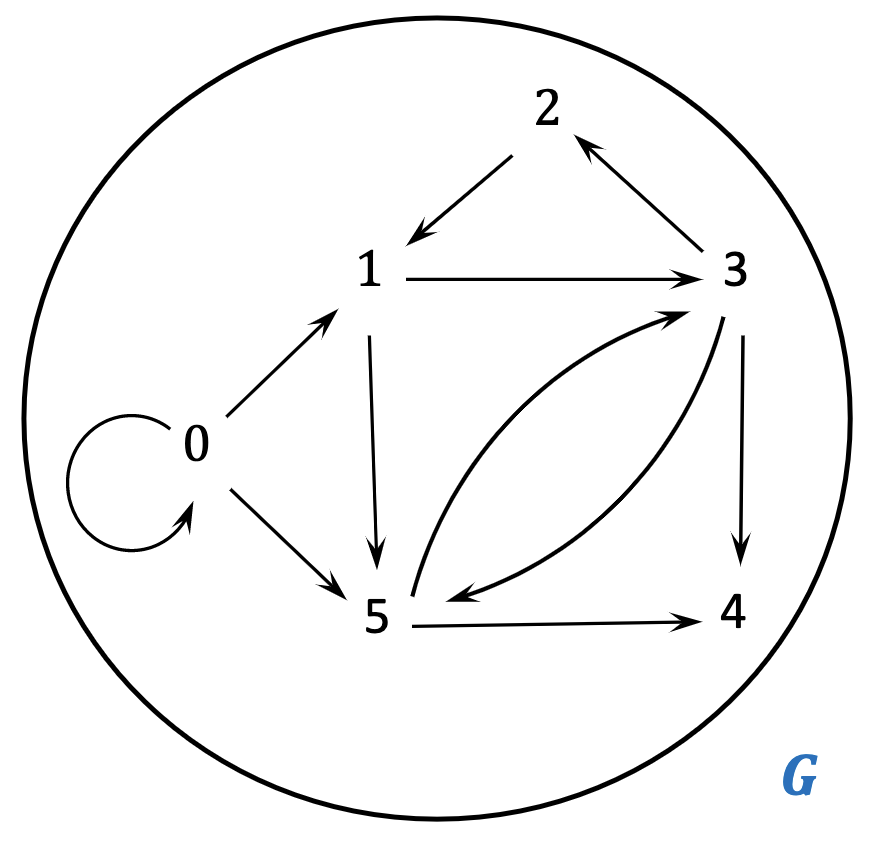
\includegraphics[width=3.3cm]{images/esempio-grafo.png}
        \caption{}
    \end{subfigure}
    \hfill
    \begin{subfigure}{.3\textwidth}
        \centering
        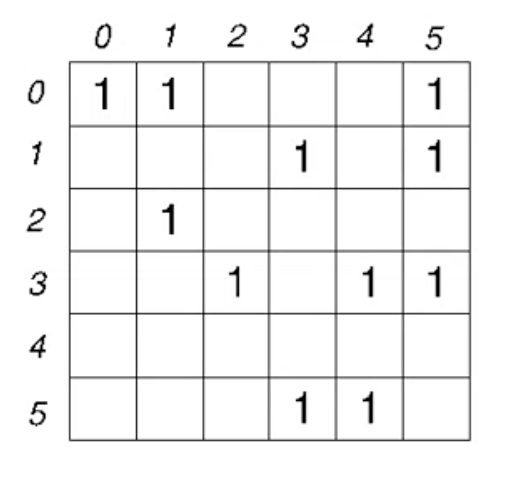
\includegraphics[width=3.3cm]{images/matrice-adiacenza.png}
        \caption{}
    \end{subfigure}
    \hfill
    \begin{subfigure}{.3\textwidth}
        \centering
        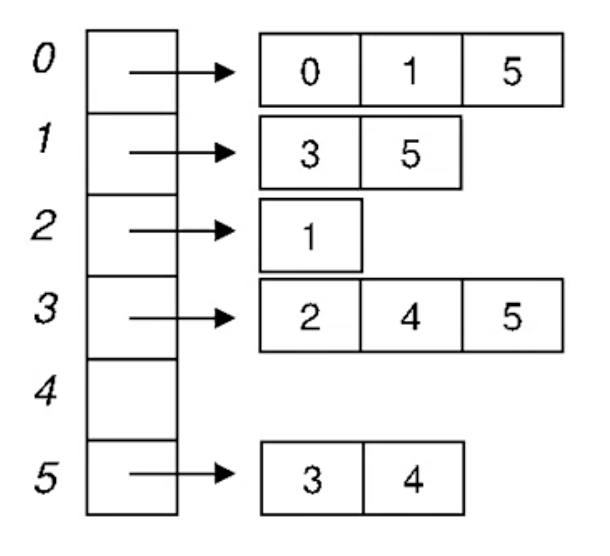
\includegraphics[width=3.3cm]{images/liste-adiacenza.png}
        \caption{}
    \end{subfigure}
    \vspace{-5pt}
    \caption{In (a) il grafo, in (b) la matrice di adiacenza ed in (c) la lista di adiacenza}
\end{figure}
\subsubsection{Matrici di adiacenza}
Una delle tecniche di rappresentazione di un grafo è tramite una matrice di adiacenza.
\begin{definition}[Matrice di adiacenza]
    La matrice di adiacenza di $G$ è una matrice quadrata $A$ con $n$ righe e $n$ colonne, numerate da $0$ a $n-1$, dove l'elemento di $A_ij$ (in riga $i$ e colonna $j$) assume un valore in $0$ se $(i,j) \notin E$ e $1$ se $(i,j) \in E$.
\end{definition}
Questo tipo di rappresentazione è molto utile per sfruttare tecniche di algebra lineare, ma non conviene in termine di spazio occupato se ci sono pochi archi da rappresentare.\\
Alcune proprietà dei grafi viste tramite le matrici di adiacenza:
\begin{itemize}
    \item Dato $x \in V$, $N^+(x)$ si ottiene guardando tutti gli $1$ nella riga $x$.
    \item Dato $x \in V$, $N^-(x)$ si ottiene guardando tutti gli $1$ nella colonna $x$.
    \item Per ottenere $|E|$ si sommano tutti gli $1$ nella matrice.
    \item $d^+_x$ si ottiene sommando gli $1$ di una riga.
    \item $d^-_x$ si ottiene sommando gli $1$ di una colonna.
\end{itemize}

\subsubsection{Liste di adiacenza}
Un metodo alternativo alle matrici di adiacenza sono le liste di adiacenza.
\begin{definition}[Liste di adiacenza]
    La rappresentazione con liste di adiacenza di un grafo orientato $G = (V,E)$ è costituita da un array di $A$ di $n = |V|$ insiemi in cui l'elemento i-esimo è il vicinato in uscita del nodo $i \in V$, cioè $A[i] = N^+(i)$.
\end{definition}
Questo tipo di rappresentazione occupa meno memoria delle matrici di adiacenza se $|E|$ è molto minore di $|V|^2$. Questo perché se prendiamo per esempio una $|E| = 10^{11}$ ed una $|V| = 10^9$ la rappresentazioni di una matrice occuperà $|V|^2$ spazi che sono uguali a $10^{18}$ mentre le liste occuperanno spazi uguali a $|V| + |E|$ che in questo caso sarebbero $10^9 + 10^{11}$ che è minore di della rappresentazione della matrice.\\
Alcune proprietà dei grafi viste tramite le matrici di adiacenza:
\begin{itemize}
    \item Dato $x \in V$, $N^+(x)$ si ottiene leggendo semplicemente la lista di adiacenza ad $x$.
    \item Dato $x \in V$, $N^-(x)$ si ottiene leggendo tutte le di di adiacenza e cercando occorrenze di $x$.
\end{itemize}

\subsection{Grafi orientati etichettati e pesati}
\begin{definition}[Grafo etichettato, grafo pesato]
    Un grafo orientato, etichettato o pesato è una tripla $G = (V,E,L)$ dove $L$ è una funzione $L: (V \cup E) \to D$ che associa ad ogni nodo e arco una etichetta presa da un certo dominio $D$ di valori. Nel caso che $D$ sia un valore numeri il grado si chiama anche pesato.
\end{definition}
La rappresentazioni di etichette su grafi orientati è simile a quella per grafi normali, quindi si possono usare le tecniche di matrici di adiacenza e di liste di adiacenza andando però nel primo caso ad aggiungere l'etichetta al posto del numero 1, mentre nelle liste di adiacenza gli elementi dell'array conterranno una coppia di valori: il nodo a cui è collegato e il valore dell'etichetta.
\begin{figure}[h!]
    \centering
    \begin{subfigure}{.3\textwidth}
        \centering
        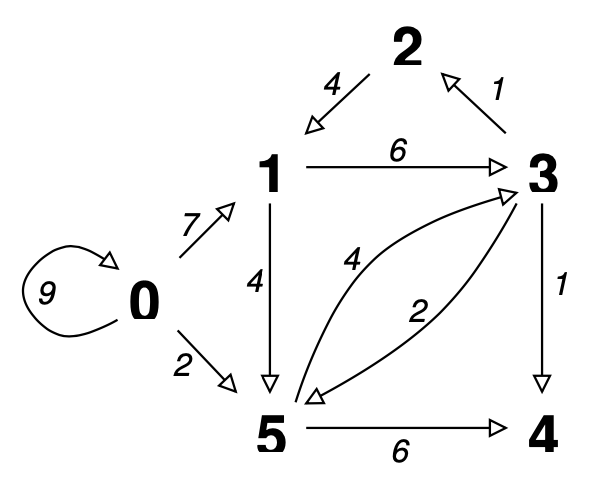
\includegraphics[width=3.5cm]{images/esempio-grafo-pesato.png}
        \caption{}
    \end{subfigure}
    \hfill
    \begin{subfigure}{.3\textwidth}
        \centering
        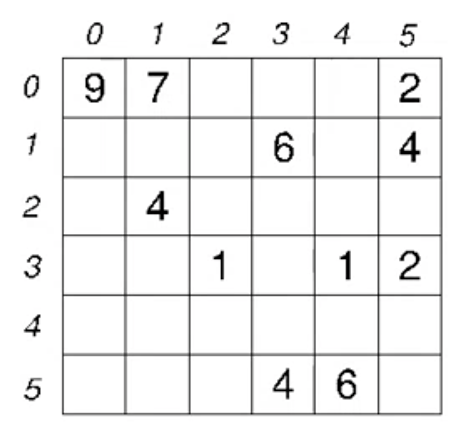
\includegraphics[width=3.5cm]{images/matrice-adiacenza-pesata.png}
        \caption{}
    \end{subfigure}
    \hfill
    \begin{subfigure}{.3\textwidth}
        \centering
        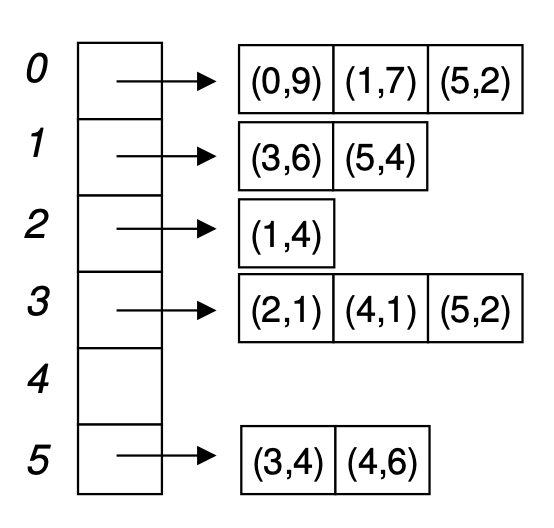
\includegraphics[width=3.5cm]{images/lista-adiacenza-pesata.png}
        \caption{}
    \end{subfigure}
    \vspace{-5pt}
    \caption{In (a) il grafo pesato, in (b) la matrice pesata ed in (c) la lista pesata}
\end{figure}

\newpage
\subsection{Cammini}
\begin{definition}[Cammino]
    Un \textbf{cammino} è una sequenza di nodi collegati da archi (nella stessa direzione).
\end{definition}

\subsubsection{Walk, trail e path}
Esistono 3 tipi di cammini: il \textbf{walk}, il \textbf{trail} ed il \textbf{path}
\begin{definition}[Walk]
    Dato un grafo orientato $G = (V,E)$ un \textbf{walk} è una sequenza di nodi.
    \begin{center}
        $P = v_0, v_1, \ldots, v_k$ tale che $(v_i,v_{i+1}) \in E$ per ogni $i \in K$
    \end{center}
\end{definition}
\hspace{-15pt}Vediamo che la \textbf{lunghezza} di $P$ è uguale a $k$ mentre gli estremi di un walk $P$ sono $v_0$ e $v_k$, e si dice che $P$ inizia con $v_0$ e termina con $v_k$.
\begin{note}
Un walk di lunghezza $0$ è un semplice nodo.
\end{note}

\begin{definition}[Trail e path]
    Un walk $P$ è detto \textbf{trail} se attraversa ogni arco in $E$ al più una volta. Un trail è detto \textbf{path} se attraversa ogni nodo in $V$ al più una volta.
\end{definition}

\begin{example}
    Prendendo come esempio l'immagine \ref{fig:esempio-grafo} vediamo che:
    \begin{itemize}
        \item La sequenza $\{0, 0, 1, 3, 2, 1, 3, 2\}$ è un walk ma non è un trail.
        \item Mentre la sequenza $\{0, 0, 1, 3, 4, 3, 4\}$ è un trail ma non è un path.
        \item Infine la sequenza $\{0, 1, 3, 4\}$ è un path.
    \end{itemize}
\end{example}

\subsubsection{Enunciati sui cammini}
\begin{proposition}\label{proposizione-walk-1}
Sia $G = (V,E)$ un grafo orientato e siano $x,y \in V$ due nodi. Allora vale che:
\begin{center}
    \footnote{Ricorda che $E^n$ è una composizione di$ $E per $n$ volte, quindi con $n=3$ è $E;E;E$}Esiste un walk di lunghezza $n\in \mathbb{N}$ da $x$ a $y$ $\Longleftrightarrow (x,y) \in E^n$
\end{center}
\end{proposition}
\begin{demostration}
Dimostrammo la proposizione \ref{proposizione-walk-1} per induzione.
\begin{enumerate}
    \item \underline{Caso base:} con $n=0$ può esistere un solo walk di lunghezza 0 e sarebbe un walk $(x,x)$ con il nodo $x \in V$. Questo caso si dimostra facilmente visto che $E^0 = Id_E$ e per definizione di identità $(x,x) \in Id_E$.
    \item \underline{Passo induttivo:} Per ipotesi induttiva assumiamo che il caso per un walk di lunghezza $n$ sia vero, dimostriamo ora che vale anche quello di lunghezza $n+1$. \\ \\
    Noi sappiamo che esista un walk di lunghezza $n + 1$ fra $x$ e $y$:
    \begin{enumerate}
        \item $\Longleftrightarrow \: \exists$ un walk $x, v_1, v_2, ..., v_n, y$ che a sua volta esiste.
        \item $\Longleftrightarrow (x, v_1) \in E$ ed esiste un walk $v_1, v_2, ..., v_n, y$, che esiste.
        \item $\Longleftrightarrow (x, v_1) \in E$ e $(v_1,y) \in E^n$.
        \item $\Longleftrightarrow (x,y) \in E^{n+1}$
    \end{enumerate}
    Nel (c) il primo passaggio del walk deve esistere già in $E$ ($E$ senza ulteriori composizioni$E^n$), il resto del walk invece è $(v_1,y) \in E^n$ e non in $n+1$ perché avendo "tolto" e messo a se il primo passo ($(x, v_1) \in E$) ci rimane un cammino di lunghezza $n$. Se quindi facciamo la composizione fra $E$ ed $E^n$ ($E;E^n$) torna che è uguale a dire $E^{n+1}$, quindi arriviamo al punto (d) che dimostra il passo induttivo. $\blacksquare$
\end{enumerate}
\end{demostration}

\newpage
\begin{lemma}\label{lemma-1}
    Sia $G=(V,E)$ un grafo orientato e siano $x,y \in V$ due nodi. Allora vale che:
    \begin{enumerate}
        \item Se esiste un walk da x a y $\Longrightarrow$ esiste un trail da x a y.
        \item Se il walk ha lunghezza $>0$, allora anche il trail ha lunghezza $>0$.
    \end{enumerate}
\end{lemma}
\begin{demostration}
Questo lemma può essere dimostrato intuitivamente in entrabi i suoi punti. \\ \\
\underline{Caso 1:} Innanzitutto partiamo da un walk P = 1,2,3,4,1,2,6,5 dove c'è almeno una ripetizione dello stesso arco (in questo caso si passa 2 volte fra 1,2) che quindi non lo rende un trail.\\
Possiamo però rendere questo walk un trail rimuovendo tutti i collegamenti da una all'altra coppia ripetuta (in questo caso si rimuove "3,4,1,2") visto che se 2 è connesso a 6 possiamo connetterlo direttamente senza passare per 3,4,1,2. Eseguendo questa operazione per tutte le ripetizioni otteniamo un trail. \\\\
\underline{Caso 2:} Se esiste un walk di lunghezza maggiore di 0 fra $x$ e $y$, come visto sopra, esisterà anche un trail fra $x$ e $y$, ma è immediato dire che se esiste un trail fra questi due nodi deve esistere almeno un arco che li collega e che quindi dimostra che la lunghezza è $>0$.
$\blacksquare$
\end{demostration}
\begin{figure}[h!]
    \centering
    \begin{subfigure}{.3\textwidth}
        \centering
        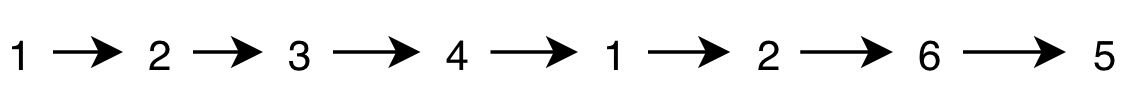
\includegraphics[width=5cm]{images/lemma-walk-trail-3.png}
        \caption{}
    \end{subfigure}
    \hfill
    \begin{subfigure}{.3\textwidth}
        \centering
        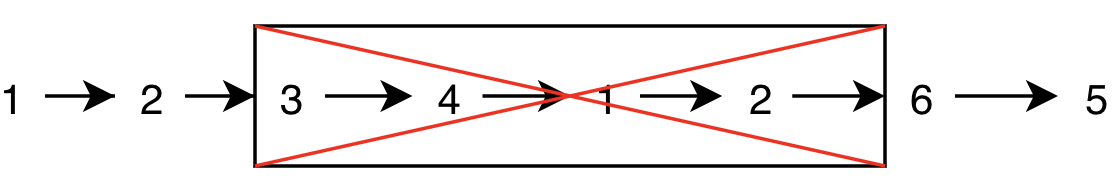
\includegraphics[width=5cm]{images/lemma-walk-trail-2.png}
        \caption{}
    \end{subfigure}
    \hfill
    \begin{subfigure}{.3\textwidth}
        \centering
        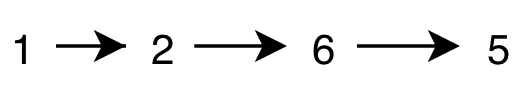
\includegraphics[width=3.5cm]{images/lemma-walk-trail-1.png}
        \caption{}
    \end{subfigure}
    \vspace{-5pt}
    \caption{Steps di trasformazione di un walk in un trail}
\end{figure}

\begin{lemma}\label{lemma-2}
Sia $G=(V,E)$ un grafo orientato e siano $x,y \in V$ due nodi. Allora vale che:
\begin{center}
    Se esiste un trail da x a y, allora esiste un path da x a y.
\end{center}
\end{lemma}
\begin{demostration}
Pure questo lemma si dimostra in maniera abbastanza intuitiva. Se prendiamo infatti un trail P = 4,5,6,7,6,9 che avendo una ripetizione di un nodo (il 6) non è un path, possiamo però farlo diventare andando a costruire un path rimuovendo il nodo ripetuto insieme a tutti i nodi intermedi (fra i due nodi doppi) e connettere il collegamento del nodo ripetuto al nodo mantenuto, riportato a questo esempio rimuoviamo 7,6 e connettiamo 9 a 4,5,6, questo fa uscire un path 4,5,6,9. Nel caso che con questa operazioni non sia ancora uscito un path basta ri-eseguirla per tutti i nodi ripetuti che rimangono. $\blacksquare$
\end{demostration}
\begin{figure}[h!]
    \centering
    \begin{subfigure}{.3\textwidth}
        \centering
        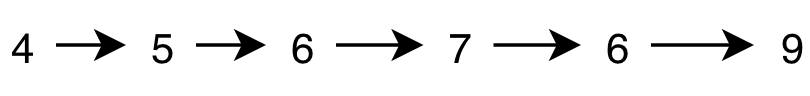
\includegraphics[width=5cm]{images/trail-path-1.png}
        \caption{}
    \end{subfigure}
    \hfill
    \begin{subfigure}{.3\textwidth}
        \centering
        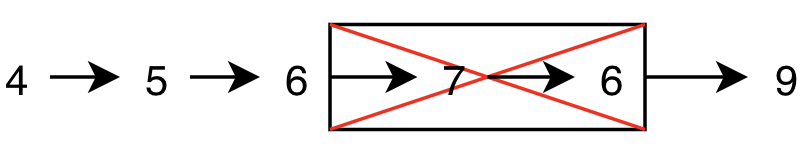
\includegraphics[width=5cm]{images/trail-path-2.png}
        \caption{}
    \end{subfigure}
    \hfill
    \begin{subfigure}{.3\textwidth}
        \centering
        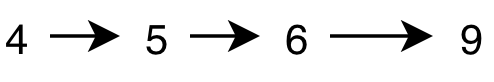
\includegraphics[width=3.5cm]{images/trail-path-3.png}
        \caption{}
    \end{subfigure}
    \vspace{-5pt}
    \caption{Steps di trasformazione di un trail in un path}
\end{figure}

\subsubsection{Walk chiusi, circuiti, cicli}
Quando in un walk si parte e si termina sullo stesso nodo possiamo andare a definire tale cammino in uno di questi 3 modi.
\begin{definition}[Walk chiuso, circuito e ciclo]\label{walk-chiusi-circuiti-cicli}
    Dato un walk P esso si definisce \textbf{walk chiuso} se gli estremi sono lo stesso nodo. Un walk chiuso che è un trail si definisce \textbf{circuito}, mentre un circuito che è un path viene chiamato \textbf{ciclo} (Senza considerare gli estremi).
\end{definition}
\begin{definition}[Grafo ciclico]
    Un grafo G si dice \textbf{ciclico} se esiste almeno un ciclo in G, in caso contrario di dice aciclico
\end{definition}

\newpage
\begin{proposition}\label{proposizione-walk-2}
    Sia G = (V,E) un grafo orientato e x un nodi in V. Le seguenti affermazioni sono equivalenti:
    \begin{enumerate}
        \item Esiste un walk chiuso da x a x.
        \item Esiste un circuito da x a x.
        \item Esiste un ciclo da x a x.
        \item $(x,x) \in E^*$
    \end{enumerate}
\end{proposition}
\begin{demostration}
Anche questa proposizione si dimostrazione intuitivamente applicando gli enunciati visti prima. Innanzitutto partiamo a dimostrare che se (1) allora (2). Questa affermazione è vera per la proposizione \ref{lemma-1}. Dimostriamo ora che se (2) allora (3). Questo si dimostra rapidamente come prima applicando una proposizione vista in precedenza, in questo caso la \ref{lemma-2}. In fine per la proposizione \ref{proposizione-walk-1} (1) se e solo se (4). E così dimostrato che queste 4 affermazioni si equivalgono. $\blacksquare$
\end{demostration}


\subsection{Connettività}
\begin{definition}[Fortemente connesso]\label{grafo-fortemente-connesso}
    Dato un grafo orientato $G = (V,E)$ si dice che questo grafo è \textbf{fortemente connesso} se per ogni coppia di nodi $x,y \in V$ esiste un walk da $x$ a $y$.
\end{definition}
\begin{definition}[Componente fortemente connesso]\label{componente-fortemente-connesso}
    Una componente fortemente connessa (SCC) di $G$ è un sottoinsieme non vuoto di nodi $U \subseteq V$ tale che:
    \begin{enumerate}
        \item Per ogni coppia di nodi $x,y \in U$ esiste un walk da $x$ a $y$.
        \item Se esiste un $U' \subseteq V$ che soddisfa la $1$ e $U \subseteq U'$, allora $U = U'$ \footnote{$U$ si definisce sottoinsieme massimale}.
    \end{enumerate}
\end{definition}
\begin{example}
    Prendiamo per esempio l'immagine \ref{fig:esempio-SCC}:
\end{example}
\begin{wrapfigure}[9]{l}{6cm}
    \vspace{-10pt}
    \centering
    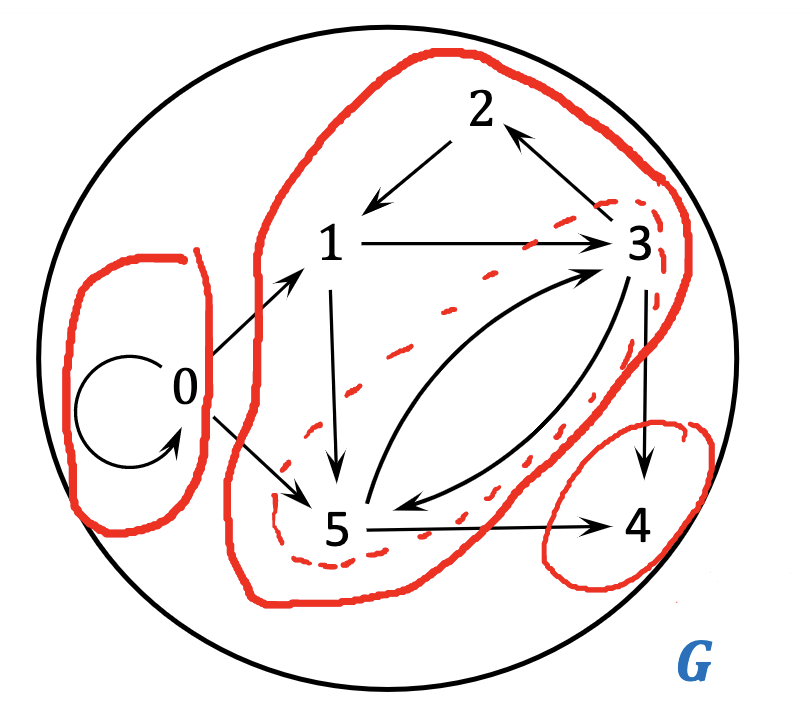
\includegraphics[width=3.7cm]{images/esempio-SCC.png}
    \caption{Grafo con i suoi SCC}
    \label{fig:esempio-SCC}
\end{wrapfigure}
In questa immagine vediamo che se prendiamo un sottoinsieme U = $\{5,4\}$ esso non è un SCC perchè non è validato il punto (2) visto che esiste un sottoinsieme $U' = \{1,3,5\}$ che lo contiene. \\Anche $U'$ non è un SCC mentre se prendiamo come $U = \{1,2,3,5\}$ questo è un SCC visto che c'è un walk per ogni elemento ed è il sottoinsieme massimale.\\
In questo esempio risulta che i SCC sono: 
\begin{center}
    $\{1,2,3,5\}$, $\{4\}$, $\{0\}$
\end{center}

\subsubsection{Componenti connesse e partizioni}
\begin{proposition}
    Dato un grafo $G=(V,E)$, l'insieme delle componenti fortemente connessi di $G$ è una partizione di $V$.
\end{proposition}
\begin{demostration}
Andiamo ora a dimostrare questa proposizione. Innanzitutto ricordiamo che $P = \{A_i\}_{i \in I}$ è una partizione dell'insieme $A$ se rispetta queste 3 condizioni:
\begin{enumerate}
    \item $\forall i$ $A_i \neq \O$
    \item $\bigcup^m_{i=1}A_j = A$
    \item $\forall i, j A_i \cap A_j = \O$ con $i \neq j$
\end{enumerate}
Quello che noi dobbiamo dimostrare è che l'insieme SCC = $\{C_1, C_2, \ldots, C_k\}$ è un partizione di $G$.
\begin{enumerate}
    \item La prima si dimostra immediatamente, perché un componente fortemente connesso non può essere vuoto per la sua definizione \ref{componente-fortemente-connesso}.
    \item Il secondo punto si dimostra prendendo una $x \in V$ e un insieme $U = \{x\}$, il quale rispetta la condizione (1) della definizione \ref{componente-fortemente-connesso}. Ora questo insieme può o essere una partizione, oppure esser contenuto in una componete fortemente connesso; capiamo dunque che se ripetiamo questa operazione per ogni elemento dell'insieme $V$ avremo una serie di SCC che alla peggio saranno tutti insiemi di un elemento o al meglio sarà tutto $V$, in ogni caso comunque ogni elemento apparterrà alla fine ad un SCC che se andiamo ad unire tutti insieme avremo $V$.
    \item Andiamo a dimostra il terzo punto per assurdo.\\ 
    Supponiamo che $\exists C_i, C_j$ partizioni distinte $\mid C_i \cap C_j \neq \O$. Se questa condizione è vera allora $\exists x \in C_i \cap C_j$ e $\exists y \in C_i \setminus C_j$ e anche $\exists z \in C_j \setminus C_i$ per definizione di intersezione.\\\\
    Se però la condizione che abbiamo posto per assurdo è vera allora $\forall \: y \in C_i$ e $\forall \: z \in C_j \Longrightarrow C_i \cup C_j$ soddisfa la proprietà (1) della definizione \ref{componente-fortemente-connesso}, e quindi che:\\
    $\exists$ walk $y \ldots x$, $\exists$ walk $x \ldots z \Longrightarrow \exists$ walk $y \ldots z$\\
    $\exists$ walk $z \ldots x$, $\exists$ walk $x \ldots y \Longrightarrow \exists$ walk $z \ldots y$ \\
    e questo dovrebbe avvenire perché se $C_i \cap C_j \neq \O$ vuol dire che c'è un elemento in comune in entrambi gli insieme che per la proprietà (1) dovrà avere un walk con gli altri elementi sia di $C_i$ che di $C_j$.
    Ma se ciò accadesse gli insiemi stessi $C_i$ e $C_j$ non sarebbero più partizioni perché sarebbe violata la proprietà (2) della definizione esistendo un insieme $C_i \cup C_j$ che li contiene. $\blacksquare$
\end{enumerate}
\end{demostration}

\subsubsection{Proprietà connettività}
\begin{proposition}\label{proposizione-connettività-1}
    Per tutti i grafi orientati $G=(V,E)$ e tutti gli $x,y \in V$ vale che:
    \begin{enumerate}
        \item $G$ è fortemente connesso $\Longleftrightarrow V \times V \subseteq E^*$.
        \item $(x,y) \in E^* \cap (E^*)^{op} \Longleftrightarrow$ $x$ ed $y$ appartengono alla stessa componente fortemente connessa.
    \end{enumerate}
\end{proposition}
\begin{demostration} \label{dimostrazione-prop-1}
Questo due proprietà sono vere perché:
\begin{enumerate}
    \item Nella prima dire di avere un grafo fortemente connesso vuol dire avere un grafo che per ogni $x, y \in V \times V$ nodi esiste un walk fra essi, ma ciò e vero se e solo se (per la proposizione \ref{proposizione-walk-1}) per ogni $x, y \in V \times V$ val che  $(x,y) \in E^*$\footnote{Ricorda che la stella di kleene applica la chiusura transitiva per rendere appunto transitivo l'insieme, quindi applica una sequenza di composizioni, che è lo stesso di $E^n$}, ma se ogni $(x,y)$ appartengono sia a $V \times V$ che a $E^*$ possiamo scrivere che $V \times V \subseteq E^*$ (non il viceversa perché la stella di kleene include anche la proprietà riflessiva).
    \item Per dimostrare la seconda consideriamo che se esiste un walk fra $x$ e $y$ e viceversa vuol dire che $x$ e $y$ fanno parte della stessa componente fortemente connessa e quindi $(x,y) \in E^*$ per la dimostrazione vista sopra, e $(x,y) \in (E^*)^{op}$, e questo perché: se lo vediamo come $(x,y) \in (E^{op})^*$ (possibile per le proprietà della stella di kleene) quello che facciamo è andare ad invertire tutti gli archi in E e poi aggiungere la chiusura di kleene che, aggiungendo la proprietà transitiva all'insieme, fa si che esista un walk fra (x,y); quindi in conclusione visto che ($x,y$) apparitene ad entrambi gli insiemi apparterrà anche alla loro composizione $(x,y) \in E^* \cap (E^*)^{op}$. $\blacksquare$
\end{enumerate}
\end{demostration}

\subsection{Grafo orientato aciclico (DAGs)}
\begin{definition}[DAG, Sorgenti, Pozzi]
    Un grafo orientato senza cicli si chiama \textbf{Directed Acyclic Graph (DAG)}. Al suo interno possono esistere uno o più nodi di grado di ingresso $0$ detti \textbf{sorgenti} e uno o più nodi di grado di uscita $0$ detti \textbf{pozzi}
\end{definition}

\begin{proposition}
    Se $G = (V,E)$ è un DAG, allora $E^*$ è un ordinamento parziale.
\end{proposition}
\begin{demostration}
Per dimostrare che un grafo è un DAG, allora la stella di Kleene sugli archi ($E^*$) è un ordinamento parziale. Bisogna quindi dimostrare le 3 proprietà che rendono una relazione su un insieme un ordinamento parziale, e cioè la \textbf{transitività}, la \textbf{anti-simmetria} e la \textbf{riflessività}.
\begin{itemize}
    \item \underline{Dimostrazione \textbf{transitiva} e \textbf{riflessiva}}: Queste due proprietà si dimostrano velocemente visto che la stella di Kleene aggiunge sia la proprietà transitiva che riflessiva all'insieme.
    \item \underline{Dimostrazione \textbf{anti-simmetrica}}: Per dimostrare questa proprietà basta, per il punto (4) del teorema di caratterizzazione \ref{teorema-caratterizzazione}, andare a dimostrare che $E^* \cap (E^*)^{op} \subseteq Id_V$.\\
    Ora noi sappiamo che se $(x,y) \in E^* \cap (E^*)^{op}$ esiste un walk fra $x$ e $y$ e viceversa per la proposizione \ref{proposizione-walk-1} (questo perché come anche descritto nella dimostrazione \ref{dimostrazione-prop-1} la stella di Kleene aggiunge una concatenazione di composizioni). Se poniamo per assurdo che $x \neq y$ quello che risulterebbe sarebbe un walk chiuso che attraversa entrambi, perché se esiste un walk ($x,y$) ed uno ($y, x$) esso crea un ciclo, ma questo non può essere possibili perché abbiamo supposto per ipotesi che $G$ sia un DAG. Quindi risulta che $x = y$. $\blacksquare$
\end{itemize}
\end{demostration}

\subsubsection{Ordinamento topologico}
\begin{definition}
    Dato un DAG $G = (V,E)$ un ordinamento topologico di $G$ è una biiezione $\eta: V \to n$ con $n = \{0,1,2,\ldots, n-1\}$ \footnote{Si ricorda che per la definizione vista nel capitolo 1 ogni numero naturale $n$ denota un insieme}tale che:
    \begin{equation}
        \textbf{per ogni arco } (u,v) \in E \textbf{ vale } \eta(u) < \eta(v)
    \end{equation}
\end{definition}
\hspace{-15pt}In altre parole, se disponiamo i vertici lungo una linea orizzontale in base alla loro numerazione $\eta$, in ordine crescente, otteniamo che gli archi risultano tutti orientati da sinistra verso destra
\begin{proposition}
    Ogni DAG ha almeno un ordinamento topologico, e ne possono esistere di più.
\end{proposition}

\subsection{Grafo non orientato}
\begin{definition}[Grafo non orientato]
    Un grado non orientato $G = (V,E)$ ha un insieme finito di nodi $V$ e un insieme di archi $E = P_2(V)$ dove $P_2(V) = \{X \subseteq V \mid |X| = 2\}$
\end{definition}
\begin{wrapfigure}[8]{l}{6cm}
    \vspace{-15pt}
    \centering
    \includegraphics[width=3.7cm]{images/esempio-grafo-non-orientato.png}
    \vspace{-5pt}
    \caption{Grafo G non oriento}
    \label{fig:esempio-grafo-non-orientato}
\end{wrapfigure}
La caratteristica principale dei grafi non orientati è che gli archi non hanno una direzione, quindi sono sottoinsiemi di nodi di cardinalità $2$. Scriviamo un arco fra $x$ ed $y$ come $xy \in E$, ovvero $\{x,y\} \in E$. Un grafo orientato inoltre non può avere cappi.\\ \\
Quello in figura \ref{fig:esempio-grafo-non-orientato} è un esempio di grafo non orientato. \\\\\\\\
\textbf{Notazione.} Alcune definizioni e notazioni sui grafi non orientati. Dato un grafo $G = (V,E)$ non orientato si dice che:
\begin{itemize}
    \item Il \textbf{vicinato} di un nodo $x \in V$: \hspace{.7cm} $N(x) = \{y \in V \mid xy \in E\}$
    \item Il \textbf{grado} di un nodo $x \in V$: \hspace{.7cm} $d_x = \lvert N(x)\rvert$.
\end{itemize}
\begin{definition}[Universale, Isolato]
    Un nodo $x$ si dice Univalente se è vicino di tutti i nodi quindi $N(x) \cup \{x\} = V$, mentre un nodo si dice isolato se non ha vicinato, quindi $N(x) = \O$
\end{definition}

\begin{definition}[Grafo orientato associato]
    Dato un grafo non orientato $G = (V,E)$, quindi un grafo con $E \subseteq P_2(V)$, il \textbf{grafo orientato associato} a $G$ è il grafo orientato $\widetilde{G} = (V, \widetilde{E})$, dove la relazione $\widetilde{E}$ è definita come:
    \begin{center}
        $\widetilde{E} = \{(x,y) \in V \times V \mid \{x,y\} \in E\}: V \leftrightarrow V$
    \end{center}
\end{definition}

\begin{figure}[h!]
    \centering
    \begin{subfigure}{.3\textwidth}
        \centering
        \includegraphics[width=3.5cm]{images/grafo-non-orientato.png}
        \vspace{-5pt}
        \caption{}
    \end{subfigure}
    \hspace{1cm}
    \begin{subfigure}{.3\textwidth}
        \centering
        \includegraphics[width=3.5cm]{images/grafo-orientato-associato.png}
        \vspace{-5pt}
        \caption{}
    \end{subfigure}
    \caption{In (a) il grafo non orientato ed in (b) il rispettivo grafo non associato}
\end{figure}

\subsubsection{Hand-shaking lemma}
	L'hand-shaking lemma varia per i grafi non orientatati rispetto a come era definito per quelli orientati.
\begin{lemma}[Hand-shaking lemma]
    Per ogni grafo non orientato $G = (V,E)$, vale che:
    \begin{center}
        $\sum\limits_{x \in V}d_x = 2\lvert E\rvert$
    \end{center}
    Esso dice infatti che la somma dei gradi di tutti i nodi è uguale a $2$ volte il numero di archi del grafo. 
\end{lemma}
Il lemma è valido perché: osservando che con l'aggiunta di un arco in un grafo si va a incrementare di $1$ il grado di $2$ nodi differenti, visto che un arco dovrà per forza connettere due nodi che non possono essere lo stesso (non esistendo il cappio), aumenterà di $2$ volta la somma di tutti i gradi, mentre aumenterà solo di $1$ il numero di archi, avendo aggiunto un solo arco, basta dunque andare a moltiplicare per $2$ il numero di archi per ottenere la somma dei gradi.

\subsubsection{Rappresentazione grafi non orientati}
Le rappresentazioni per i grafi non orientati sono similari a quelle dei grafi orientati. Esiste infatti sia la rappresentazione tramite \textbf{matrice di adiacenza} che tramite \textbf{lista di adiacenza}; le uniche differenze sono che, non esistendo un verso per gli archi, verranno riscritti $2$ volte i collegamenti, uno per ogni direzione, questo sia nelle matrici che nelle liste.
\begin{figure}[h!]
    \centering
    \begin{subfigure}{.3\textwidth}
        \centering
        \includegraphics[width=3.3cm]{images/esempio-grafo-non-orientato.png}
        \caption{}
    \end{subfigure}
    \hfill
    \begin{subfigure}{.3\textwidth}
        \centering
        \includegraphics[width=3.3cm]{images/matrice-grafo-non-orientato.png}
        \caption{}
    \end{subfigure}
    \hfill
    \begin{subfigure}{.3\textwidth}
        \centering
        \includegraphics[width=3.3cm]{images/lista-grafo-non-orientato.png}
        \caption{}
    \end{subfigure}
    \vspace{-5pt}
    \caption{In (a) il grafo non orientato, in (b) la matrice ed in (c) la lista di adiacenza}
\end{figure}

\subsubsection{Cammini nei grafi non orientati}
\begin{definition}[Walk]
    In un grafo non orientato $G = (V,E)$, un walk è una sequenza di nodi
    \begin{center}
        $P = v_0, \ldots, v_k$ tale che $\{v_i, v_i+1\} \in E$ per ogni $i \in K$
    \end{center}
    La lunghezza del walk $P$ è uguale a $k$.
\end{definition}

\begin{definition}[Trail, path]
    Si definisce trail un walk che non attraversa due volte lo stesso arco. Un path è un walk (o trail) che non attraversa due volte lo stesso nodo.
\end{definition}

Le proposizioni \ref{proposizione-walk-1}, \ref{proposizione-walk-2} e i lemmi \ref{lemma-1}, \ref{lemma-2}  sono validi in ugual modo per i grafi non orientati, bisogna solo tenere in considerazione il fatto che in questo tipo di grafi gli archi non hanno verso (in pratica bisogna sostituire la $E$ con $\widetilde{E}$), le dimostrazioni sono similari.

\subsubsection{Cicli e connettività nei grafi non orientati}
Per i grafi non orientati le definizioni di \textbf{walk chiuso}, \textbf{circuiti} e \textbf{cicli} sono uguali a quelli visti nei grafi orientati (Definizione \ref{walk-chiusi-circuiti-cicli}).
\begin{note}
Un walk chiuso (da $x$ a $x$) non implica un circuito (da $x$ a $x$), ma un circuito implica un ciclo
\end{note}
Ugualmente le definizioni di grafo \textbf{fortemente connesso} e  di \textbf{componente fortemente connesso} sono analoghe a quelle viste per i grafi orientati (Definizioni \ref{grafo-fortemente-connesso}, \ref{componente-fortemente-connesso}).\\
Anche qui, la proposizione \ref{proposizione-connettività-1} vale  per i grafi non orientati (bisogna sostituire la $E$ con $\widetilde{E}$).


\subsection{Cammini Euleriani}
\begin{definition}[Circuito e trail euleriano]
    Dato un grafo non orientato connesso $G = (V,E)$, un \textbf{circuito euleriano} è un circuito che passa esattamente una volta per tutti gli archi del grafo. Analogamente un \textbf{trail euleriano}. (conosciuto anche come percorso euleriano)
\end{definition}
Questa definizione parte del problema dei sette ponti di Konigsberg.
\begin{theorem}[Il teorema di Eulero]
Dato un grafo $G = (V,E)$ non orientato e connesso:
\begin{enumerate}
    \item Esiste un circuito euleriano $\Longleftrightarrow$ tutti i nodi hanno grado pari.
    \item Esiste un trail euleriano da $x$ a $y$, con $x \neq Y$ $\Longleftrightarrow$ $x$ a $y$ sono gli unici nodi di grado dispari.
\end{enumerate}
\end{theorem}

\begin{demostration}
Dimostrazione dei due punti del teorema di Eulero.\\\\
\underline{Punto (1)}: Per andare a dimostrare questo punto dobbiamo dimostrare i due sensi della freccia.
\begin{itemize}
    \item Se esiste un circuito euleriano $\Longrightarrow$ tutti i nodi hanno grado pari.\\
    Questo caso è facilmente dimostrabile perché: possiamo notare che ogni volta che in un circuito euleriano noi passiamo per un nodo ($x \to y \to z$) attraversiamo $2$ archi mai attraversati, questo vuol dire che il numero di archi incidenti\footnote{Ricorda che gli archi incidenti sono gli archi che escono/entrano in un nodo, in un grafo non orientato} in un nodo è il doppio delle volte in cui il circuito ci passa, inoltre non può verificarsi una casistica in cui un nodo ha solo un arco perché in quel modo non ci verificherebbe un circuito.\\ Essendo che il numero di archi incidenti ad un nodo è il doppio non potrà mai essere un numero dispari.
    \item Se tutti i nodi hanno grado pari $\Longrightarrow$ esiste un circuito euleriano.\\
    Innanzitutto prendiamo un nodo $r$ ed iniziamo a creare un percorso in G marcando ogni arco in cui passiamo in modo da non passarci una seconda volta, a questo punto solamente $r$ avrà un solo arco incidente marcato all'inizio, mentre ogni nodo in cui passiamo avrà due archi marcati (un per arrivarci ed uno per andare), continueremo finché non ritorneremo nel nodo $r$ creando un circuito, non potrà essere altrimenti perché se il nodo finale $u \neq r$ allora vorrebbe dire che ha un numero di archi incidenti dispari (avendo un arco per arrivarci e non uno per uscirci) e questo non è possibile per ipotesi.\\\\
    A questo punto chiamiamo il circuito trovato C, se C passa per tutti gli archi allora è euleriano ed abbiamo finito, in caso contrario dobbiamo utilizziamo l'ipotesi che G sia connesso per così dedurre che esista un nodo $r'$ in C che ha un arco incidente non marcato.\\\\ 
    Prendiamo ora $r'$ e ripetiamo l'operazione vista prima andando a ricreare un nuovo circuito $C'$, notiamo che $C'$ e $C$ sono disgiunti sugli archi (perché marchiamo man mano gli archi che passiamo), inoltre $C$ e $C'$ si incontreranno in $r'$. \\\\
    A questo punto avremo due circuiti $C$ e $C'$ che coincidono in un nodo $r'$ e con tutti archi disgiunti, se quindi andiamo ad unire questi due circuiti prendendo come nodo di partenza e di arrivo $r'$ avremo un circuito che o è euleriano o avrà un nodo $r''$ con un arco non segnato, vediamo dunque che possiamo nuovamente ripetere l'operazione precedentemente vista altre $n$ volte, andando volta in volta a combinare i circuiti trovati fino a che non si creerà un circuito euleriano. $\blacksquare$
\end{itemize}
\underline{Punto (2)}: Anche qui bisogna dimostrare i due sensi della freccia per dimostrare la sua veridicità.
\begin{itemize}
    \item Se esiste un trail euleriano da $x$ a $y$, con $x\neq y \Longrightarrow$ $x$ e $y$ sono gli unici nodi di grado dispari.\\
    Questo verso lo dimostriamo vedendo che ogni volta che attraverso un nodo $v$ utilizzo $2$ archi, uno per entrare ed uno per uscire, le uniche eccezioni sono per il nodo di partenza e per quello di arrivo che avranno grado uguale a $2k + 1$ dove $k$ è il numero di volte in cui si passa per quel nodo (esclusa la partenza o l'arrivo) ed il $+1$ indica appunto la partenza nel caso di $x$ e l'arrivo nel caso di $y$. Abbiamo così dimostrato il primo verso.
    \item Se $x$ e $y$ sono gli unici nodi di grado dispari $\Longrightarrow $ esiste un trail euleriano da $x$ a $y$.\\
    Prendiamo per dimostrare questo caso un grado G = (V,E) che sua un grado connesso con $x,y \in V$ di grado dispari e $\forall v \in V . v\notin \{x,y\}$ siano di grado pari (queste condizioni sono vere per l'ipotesi).\\
    Ora creiamo un nuovo grafo $G'$ uguale a G solo introducendo un nuovo nodo $z$ con due archi $\{z,x\}$ e $\{z,y\}$ (questo nuovo nodo rispetta le condizioni poste nell'ipotesi). \\
    $G'$ è connesso visto che il nodo $z$ è connesso ad almeno un nodo il quale, appartenendo anche al grafo G che era connesso per ipotesi, è collegabile a tutti gli altri nodi, dunque che $z$ lo sarà, e quindi $G'$ è connesso.\\
    Essendo che $G'$ + connesso tutti, tutti i odi hanno grado pari $\exists$ circuito euleriano per il punto (1) di questo teorema. Ma visto che esiste un circuito euleriano $z,x,\ldots,y,z$ esisterà allora un trail $x,..,y$ che sarà euleriano nel caso si consideri il grafo $G$ (quindi senza $z$ e i suoi archi). Così dimostriamo anche questa implicazione. $\blacksquare$
\end{itemize}
\end{demostration}

\subsection{Cicli e path Hamiltoniani}
\begin{definition}[Cicli e path Hamiltoniani]
    Dato un grafo connesso (orientato o non orientato), un \textbf{ciclo hamiltoniano} è un ciclo che passa esattamente una volta per tutti i nodi del grafo. Analogamente, path hamiltoniano.
\end{definition}
Questo tipo di cammino non prevede una caratterizzazione semplice come per i circuiti euleriani. Equivale inoltre a cercare una permutazione dei nodi che formano un path.

\subsubsection{Il problema del commesso viaggiatore}
Il problema del commesso viaggiatore consiste, dato un grafo pesato non orientato, di trovare un ciclo hamiltoniano di peso minimo, dove il peso è la somma dei pesi degli archi attraversati.
\begin{figure}[h!]
    \centering
    \begin{subfigure}{.3\textwidth}
        \centering
        \includegraphics[width=3.3cm]{images/es-problema-viaggiatore-1.png}
        \caption{}
    \end{subfigure}
    \hfill
    \begin{subfigure}{.3\textwidth}
        \centering
        \includegraphics[width=3.3cm]{images/es-problema-viaggiatore-2.png}
        \caption{}
    \end{subfigure}
    \hfill
    \begin{subfigure}{.3\textwidth}
        \centering
        \includegraphics[width=3.3cm]{images/es-problema-viaggiatore-3.png}
        \caption{}
    \end{subfigure}
    \caption{(a) il grafo pesato, (b) ciclo hamiltoniano in (c) un ciclo hamiltoniano di peso minimo}
\end{figure}

\subsection{Distanze}
\begin{definition}[Distanza]
    Una \textbf{distanza} (o metrica) su un insieme A è una funzione $d: A \times A \to \mathbb{R}$ che soddisfa le seguenti proprietà per ogni $x,y,z \in A$.
    \begin{enumerate}
        \item $d(x,y) \geq 0$.
        \item $d(x,y) = 0 \Longleftrightarrow x = y$.
        \item $d(x,y) = d(y,x)$ (simmetria).
        \item $d(x,y) \leq (x,z) + d(z,y)$ (disuguaglianza triangolare)
    \end{enumerate}
\end{definition}
Si può notare che tutte queste condizioni sono soddisfatte dalla distanza euclidea \footnote{Ricorda che la distanza euclidea è la distanza fra due punti in un piano cartesiano}, infatti (1) la distanza euclidea è sempre maggiore o uguale a 0, e se è 0 è perché abbiamo preso due punti uguali (2), inoltre (3) la distanza fra due elementi non cambia, indipendentemente da quale punto prendiamo per prima, ed in fine in un triangolo la somma delle lunghezze di due lati  maggiore o uguale a quella del terzo lato (4).

\begin{definition}[Distanza su un grafo non orientato]
    Sia $G = (V,E)$ un grafo non orientato connesso. Dati due nodi $x,y \in V$, la loro \textbf{distanza} $d(x,y)$ è la lunghezza del walk più breve tra $x$ e $y$ (il cammino minimo).
\end{definition}
Possiamo vedere che in quest'ultima definizione sono rispettate i quattro punti della definizione di distanza.
\begin{enumerate}
    \item La distanza fra $x$ e $y$ è sempre $\geq 0$ perché in caso contrario vorrebbe dire che non esiste, e ciò non è possibile per la definizione stessa (nella definizione diciamo che il grafo è connesso).
    \item Se la distanza fra due nodi è $0$ allora il nodo è lo stesso.
    \item Se esiste un cammino da $x$ a $y$ con una certa distanza, questo cammino può essere percorso anche da $y$ a $x$ e quindi mantiene la stessa distanza.
    \item Essendo la distanza la lunghezza del walk più breve la distanza fra $x$ e $y$ sarà per forza minore o uguale di quella fra $x$ e $z$ sommata con quella fra $z$ e $y$.
\end{enumerate}

\begin{definition}[Distanza su grafo induttivamente]
    Sia $G = (V,E)$ un grafo non orientato connesso. Dati due nodi $x,y \in V$, al loro distanza $d(x,y)$ può essere definita induttivamente:
    \begin{itemize}
        \item \underline{Caso base}: $d(x,y) = 0$, se $x = y$.
        \item \underline{Passo induttivo}: $d(x,y) = 1 + min\{d(z,y) \mid z\in N(x)\}$. Dove $N(x)$ è il vicinato di $x$
    \end{itemize}
\end{definition}

La definizione di distanza (come lunghezza del cammino minimo) si può applicare anche a grafi orientati fortemente connessi, ma in questo caso non vengono rispettate tutte le proprietà:
\begin{enumerate}
    \item $d(x,y) \geq 0$ è vera per la definizione di grafo fortemente connesso.
    \item $d(x,y) = 0$ se e solo se $x = y$ è vera perché l'unico cammino di lunghezza $0$ è quello fra un nodo e se stesso.
    \item $d(x,y) = d(y,x)$ invece non è rispetta perché essendoci un verso negli archi possono esistere percorsi più brevi differenti.
    \item Visto che il punto (3) non è verificato non è necessario verificare il (4).
\end{enumerate}
Nel caso di grafi fortemente orientati definiamo la funzione della distanza una quasi-metrica.

\begin{proposition}\label{proposizione-distanza-1}
    Sia $G = (V,E)$ un grafo orientato connesso e $x$ un nodo. Sia $y$ un nodo a distanza massima da $x$, allora $G\setminus \{y\}$ è connesso.
\end{proposition}

\begin{demostration}
    Dimostriamo la proposizione scritta sopra, essa dice che:
    \begin{center}
        $\forall v \in V, d(x,y) \geq d(x,v) \Longrightarrow \forall v \in V \setminus \{y\}$ $\exists$ path $P = x,\ldots,v$. che non include y.
    \end{center}
    I path $P = x,\ldots,v$ non devono includere y perché se lo includesse allora $\exists$ $P' = x\ldots,y$ più corto di $P$ e questo contraddice che $d(x,y) \geq d(x,v)$.\\
    Se dal nostro grafo rimuovo y segue per quanto detto prima che $\forall v \in V \setminus \{y\}$ esiste ancora un path $P = x,\ldots,v$.
    Allora vediamo che $\forall v,w$ $\exists$ walk $W = v,\ldots,x,\ldots,w \Longrightarrow G \setminus \{y\}$ è connesso. $\blacksquare$
\end{demostration}

\subsubsection{Diametro, altezza, profondità}
\begin{definition}[Diametro di grafo]
    Il diametro di un grafo $G$ (oriento o meno) è la massima distanza tra coppie di nodi:
    \[diam(g) = \max_{x,y \in V}d(x,y)\]
\end{definition}

\begin{definition}[Profondità, altezza di nodi, albero pieno]
    Dato un albero radicato, la \textbf{profondità} di un nodo $x$ è la distanza $d(x,t)$ dalla radice $r$, e \textbf{l'altezza} di $x$ è la massima distanza tra $x$ e le sue foglie discendenti. L'altezza dell'albero è l'altezza della radice. Inoltre definiamo un albero cardinale come \textbf{pieno} se è completo e le foglie sono tutte alla stessa distanza dalla radice.
\end{definition}



\newpage
\subsection{Alberi}

\begin{definition}[Albero, foglia]
    Un \textbf{albero} è un grafo non orientato connesso, aciclico e non vuoto (con almeno $1$ nodo).
    I nodi interni hanno quindi grado $>1$ mentre i nodi di grado $1$ sono detti \textbf{foglie}.
\end{definition}

\begin{definition}[Foresta]
    Una \textbf{foresta} è un grafo non orientato, aciclico e non vuoto dove ogni componente connessa è un albero assestante.
\end{definition}
\hspace{-15pt}Da queste definizioni possiamo dedurre alcune proprietà relative agli alberi.
\begin{wrapfigure}[8]{r}{7cm}
    \centering
    \includegraphics[width=5cm]{images/es-albero.png}
    \vspace{-5pt}
    \caption{Esempio di albero}
\end{wrapfigure}
\begin{itemize}
    \item Il numero di path possibili fra due nodi è sempre uno, perché se esistessero due path distinti la concatenazione di questi due path sarebbe un walk chiuso e quindi il grafo avrebbe cicli (ricorda la proposizioni \ref{proposizione-walk-2} che ci dice che dire walk chiuso o ciclo è analogo).
\end{itemize}

\begin{itemize}
    \item Se andiamo a toglie un arco in un albero si andrà a creare una foresta con 2 alberi.
    \item Se invece andiamo ad aggiungere un arco quello che uscirà non sarà più un albero perché si creerà un ciclo.
\end{itemize}


\begin{proposition}
    Dato un albero G = (V,E) con $n = |V|$ nodi, valgono le seguenti proprietà:
    \begin{enumerate}
        \item Se $n \geq 2$ (ovvero l'albero ha almeno due nodi), allora G ha almeno una foglia (ovvero un nodo di grado 1).
        \item G ha esattamente $n-1$ archi, cioè $|E| = n-1$.
        \item Per ogni coppia di nodi distinti $x,y \in V$, esiste un unico path da x a y.
        \item Per ogni arco $xy \in E$, la rimozione di $xy$ rende il grafo non connesso.
        \item Per ogni coppia di nodi distinti $x,y \in V$ tale che $xy \notin E$, l'aggiunta dell'arco xy crea un ciclo, cioè $G' = (V, E \cup {xy})$ è un ciclo.
    \end{enumerate}
\end{proposition}


\begin{demostration}
Andiamo ora a dimostrare ogni punto della proposizione sopra.
\begin{enumerate}
    \item Per dimostrare il primo punto prendiamo innanzitutto un albero T = (V,E) con almeno 2 nodi, per la proposizione \ref{proposizione-distanza-1} $\exists y \in V \: |\: T \setminus \{y\}$ è connesso $\Longrightarrow T \setminus \{y\}$ rimane connesso quindi rimane un albero.\\
    Ora, se re-introduciamo y possiamo vedere 2 casi:
    \begin{itemize}
        \item O $|N(y)| = 1$ (il vicinato di $y$ è 1), quindi $y$ è una foglia di T e la proprietà e verificata.
        \item Oppure $|N(y)| \geq 2$ (il vicinato di $y$ è maggiore o uguale a 2), in questo caso però $\exists$ path $P = w,...,z$ in $T \setminus \{y\}$ e $\exists \{z,y\}, \{y,w\} \in E$ (queste due condizioni sono previste visto che un albero è connesso), ma ciò porterebbe ad un ciclo che è impossibile.
    \end{itemize}
    Vediamo dunque che solo la prima casistica è possibile, e quindi abbiamo dimostrato questo punto. $\blacksquare$
    \item Per andare a dimostrare questo punto procediamo per induzione su n.
    \begin{itemize}
        \item \underline{Caso base:} Se n=1 allora l'albero ha un solo nodo e quindi nessun arco, la proprietà in questo caso è quindi dimostrate perché $n-1 = 0$, e $m=0$.
        \item \underline{Passo induttivo:} Assumiamo per ipotesi induttiva che la proprietà valga per tutti gli $n$ nodi, dimostriamo che vale anche per gli $n+1$ nodi. Un albero in questo caso ha almeno 1 nodo quindi $n \geq 1$ mentre nel caso $n+1$ gli alberi avranno come minimo 2 nodi ($n+1 > 1$ che è uguale a dire $n + 1 \geq 2$), per la proprietà (1) G ha almeno una foglia $y$.\\\\
        Prendiamo ora un albero $G' = G \setminus \{y\}$, togliamo dunque una foglia ed un arco (l'unico arco connesso a $y$) ed otteniamo che in $G'$ il numero di nodi $n = (n + 1)-1$ che quindi è $n = n$ ed il numero di archi è $m = (n-1)-1$ quindi $m = n$. Visto che $G'$ ha $n$ archi e $G$ ne ha $n+1$ abbiamo dimostrato l'ipotesi induttiva. $\blacksquare$
    \end{itemize}
    \item Dimostriamo questa proprietà per assurdo, quindi supponiamo che esistano due path distinsi $P_1$ e $P_2$ da $x$ a $y$. \\
    Prendiamo un nodo $z$ che sia l'ultimo nodo in comune fra $P_1$ e $P_2$ prima che $P_1$ e $P_2$ divergano in due percorsi distinti, e prendiamo un $w$ che sia invece il primo nodo dopo $z$ in $P_1$ attraversato anche da $P_2$ (l'esistenza di questi due nodi è obbligatoria perché $P_1$ e $P_2$ partono ed arrivano sugli stessi nodi, alla peggio $z = x$ e $w = y$). \\\\
    Essendo un albero un grafo connesso esisterà un cammino fra $z$ e $w$ che però sarà un ciclo perché partendo da $z$ andiamo a $w$ passando per i nodi di $P_1$ e da $w$ posso tornare a $z$ per i nodi in $P_2$; questa però è una contraddizione, è quindi verificata la proprietà. $\blacksquare$ 
    \item Questa propria si dimostra in modo veloce vedendo innanzitutto che se prendiamo un albero G con al suo interno due nodi $x$ e $y$ esisterà un unico path $P = xy$, perché in caso c'è ne fossero di più l'albero avrebbe un ciclo e quindi non sarebbe più un albero (meno di un path non è possibile per definizione di albero). Se andiamo a rimuovere P allora $\nexists$ path fra $x$ e $y$ e quindi il grafo non è connesso. $\blacksquare$
    \item Anche l'ultima proprietà si dimostra velocemente, visto che se abbiamo un albero G con due nodi $x$ e $y$ allora per definizione di albero $\exists$ path $P = x...y$ (che non sarà $xy$ per ipotesi), se aggiungiamo un arco $xy$ allora si otterrà un ciclo. $\blacksquare$
\end{enumerate}
\end{demostration}

\subsubsection{Albero radicato}
\begin{definition}[Albero radicato]
    Un \textbf{albero radicato} G=(V,E,r) è costituto da un albero G=(V,E) e da un nodo $r\in V$ chiamato \textbf{radice}.
\end{definition}

\begin{definition}[Antenato, genitore, discendete, figlio]
    Dato un albero radicato G=(V,E,r) e dato un nodo $y \in V$ e $y \neq r$ possiamo dare le seguenti definizioni.
    \begin{itemize}
        \item I nodi lungo l'unico cammino che collega y a r si chiamano \textbf{antenati}.
        \item Il primo nodo fra gli antenati (quello adiacente a y) è detto il \textbf{genitore} di y.
        \item Simmetricamente y viene detto \textbf{discendente} dei suoi antenati e \textbf{figlio} del nodo genitore.
    \end{itemize}
\end{definition}

\begin{definition}[Sottoalbero]
    Dato un albero radicato G = (V,E,r) e dato un nodo $r' \in V$ il \textbf{sottoalbero} di G con radice $r'$ è l'albero radicato G' = (V',E',r') in cui $V' \subseteq V$ contiene r' e tutti i suoi discendenti in G, e $E' \subseteq E$ contiene tutti gli archi di G tra i nodi di V'.
\end{definition}

\begin{wrapfigure}[9]{l}{7.5cm}
    \vspace{-15pt}
    \centering
    \includegraphics[width=3cm]{images/es-albero-radicato.png}
    \caption{Albero radicato con radice r}
    \label{es-albero-radicato}
\end{wrapfigure}

Se prendiamo l'immagine \ref{es-albero-radicato} vediamo che la radice $r = 0$.
La radice ha come figli 1 e 2 mentre 2 ha come antenato solo la radice.\\\\
Se prendiamo il nodo 8 questo nodo è padre di 9 e ha come fratello 7.\\
Il nodo 9 invece è un discendete di 2 essendo che 2 è un suo antenato.\\\\

\begin{definition}[Albero ordinale, albero cardinale]
    Un albero radicato si dice \textbf{albero ordinale} se per ciuscun nodo interno è definito un ordinamento totale tra i suoi figli. Un albero radicato si dice \textbf{albero cardinale} o k-ario se ogni nodo interno ha esattamente k figli, alcuni dei quali possono essere vuoti.
\end{definition}

\begin{definition}[Albero completo, binario]
    Un albero cardinale è \textbf{completo} se ogni nodo interno ha tutti e k i figli non vuoti. Un caso speciale di albero cardinale è quello con k=2, esso si dice infatti \textbf{albero binario}; in esso il primo figlio viene chiamato figlio sinistro ed il secondo figlio viene chiamato figlio destro.
\end{definition}

\subsection{Isomorfismo}
\begin{definition}[Isomorfismo]
    Dati due qualunque grafi $G_1 = (V_1, E_1)$ e $G_2 = (V_2, E_2)$ dove $\lvert V_1\rvert = \lvert V_2\rvert$ e $\lvert E_1\rvert = \lvert E_2\rvert$, un isomorfismo fra questi due  grafi è una biiezione $f: V_1 \mapsto V_2$ tra i loro nodi tale che:
    \begin{center}
        \vspace{-5pt}
        $\forall u,v \in V_1$ vale che $uv \in E_1 \Longleftrightarrow f(u)f(v) \in E_2$.
    \end{center}
\end{definition}
\hspace{-15pt}Possiamo definire due grafi isomorfi se esiste un isomorfismo fra di loro. Essere isomorfi è una relazione di equivalenza visto che sono presenti le proprietà riflessiva, simmetrica, transitiva.\\\\
Intuitivamente due grafi sono isomorfi se posso renderli identici "rinominando" i vertici, infatti la biiezione ci dice come rinominare.\\
Da aggiungere è una condizione necessaria ma non sufficiente cioè che: i nodi devono avere gli stessi grafi, infatti posso subito dire che due grafi non sono isomorfi se la sequenza dei grafi (in ordine decrescente o crescente) non è identica.
\begin{figure}[h!]
    \vspace{-5pt}
    \centering
    \begin{subfigure}{.3\textwidth}
        \centering
        \includegraphics[width=6cm]{images/esempio-isomorfismo.png}
        \vspace{-8pt}
        \caption{}
    \end{subfigure}
    \hspace{3cm}
    \begin{subfigure}{.3\textwidth}
        \centering
        \includegraphics[width=4.5cm]{images/es-non-isomorfmismo.png}
        \vspace{-5pt}
        \caption{}
    \end{subfigure}
    \vspace{-5pt}
    \caption{(a) Esempio Isomorfismo, (b) Esempio non isomorfismo}
\end{figure}

\subsection{Grafi notevoli}
Esistono una serie di grafi, detti grafi notevoli, che per la loro struttura particolare hanno preso dei nomi specifici, essi possono essere anche ritrovati di frequente in differenti casistiche in cui si utilizzano grafi.
\begin{figure}[h!]
    \vspace{-10pt}
    \begin{subfigure}{.3\textwidth}
        \centering
        \includegraphics[width=3cm]{images/clinque.png}
        \vspace{-5pt}
        \caption{Clinque}
    \end{subfigure}
    \hfill
    \begin{subfigure}{.3\textwidth}
        \centering
        \includegraphics[width=2.5cm]{images/ciclo.png}
        \vspace{-5pt}
        \caption{Ciclo}
    \end{subfigure}
    \hfill
    \begin{subfigure}{.3\textwidth}
        \centering
        \includegraphics[width=2.5cm]{images/lineare.png}
        \vspace{-5pt}
        \caption{Lineare}
    \end{subfigure}
    \hfill
    \begin{subfigure}{.3\textwidth}
        \centering
        \includegraphics[width=2.5cm]{images/griglia.png}
        \vspace{-5pt}
        \caption{Griglia}
    \end{subfigure}
    \hfill
    \begin{subfigure}{.3\textwidth}
        \centering
        \includegraphics[width=2.5cm]{images/stella.png}
        \vspace{-5pt}
        \caption{Stella}
    \end{subfigure}
    \hfill
    \begin{subfigure}{.3\textwidth}
        \centering
        \includegraphics[width=2.5cm]{images/albero-completo.png}
        \vspace{-5pt}
        \caption{Albero completo}
    \end{subfigure}
    \vspace{5pt}
    \caption{Serie di grafi notevoli}
\end{figure}
\newpage
\section{Calcolo combinatorio}

\subsection{Cardinalità insiemi}
Il calcolo combinatorio serve per dare delle risposte a domande come: quanti sono? In quanti modi? Quante possibili combinazioni?
Per questa forma di calcolo si fa molto utilizzo del concetto di cardinalità di un insieme.

\begin{definition}[Cardinalità]
La \textbf{cardinalità} di un insieme (finito) A è il numero dei suoi elementi e si indica con $|A|$.
\end{definition}

\begin{example}
$|\{a,e,i,o,u\}| = |\{i,i,i,o,u,e,a,a\}| = 5$ (Le ripetizioni non si contano)\\
$|\O| = 0$ \hspace{.7cm} $|n| = |\{0,1,2,...,n-1\}| = n$ \hspace{.7cm} $|2| = |\{0,1\}| = 2$
\end{example}

\begin{lemma}[Lemma-x]\label{lemma-x}
Dato un insieme A, sia $P = \{A_i\}_{i \in I}$ una partizione di $A$ quindi:
\begin{itemize}
    \item $\bigcup\limits_{i \in I}A_i = A$ (Punto (2) della definizione di partizione)
    \item $\forall i,j \in I . i\neq j \Longrightarrow A_i \cap A_j = \O$ (Punto (3) della definizione di partizione)
\end{itemize}
Allora vale che $|A| = \sum\limits_{i\in I}|A_i|$.
\end{lemma}
\begin{note}
Notare che nella proposizione sopra non è necessario che valga la condizione (1) di una partizione quindi che ($\forall i \in I . A_i \neq \O$), e ciò perché se consideriamo una partizione vuota essa non andrà ad influire sulla somma delle cardinalità avendo valore 0. 
\end{note}
\begin{demostration}
Per dimostrare questa proposizione supponiamo che $|A| \neq \sum\limits_{i\in I}|A_i|$, quindi $|A|$ sarà o maggiore o minore della sommatoria delle sue partizioni:
\begin{itemize}
    \item $|A| > \sum\limits_{i\in I}|A_i|$: questo caso contraddice il secondo punto della definizione di partizioni infatti fosse vero questo caso dovrebbe esistere un $a \in A$ che però $a \notin \forall i \: A_i$
    \item $|A| < \sum\limits_{i\in I}|A_i|$: questa casistica invece contraddice il terzo punto delle partizioni, infatti per far si che la cardinalità di A sia inferiore alla somma delle cardinalità delle partizioni dovrebbe esistere un $a \in A$ che contiamo due volte (ed è quindi presente in due partizioni distinte) ma questo farebbe si che $\exists A_i \neq A_j$ dove $A_i \cap A_j \neq \O$. $\blacksquare$
\end{itemize}
\end{demostration}

\subsubsection{Cardinalità di operazioni su insiemi}
\begin{proposition}
Per tutti gli insiemi A e B valgono i seguenti fatti:
\begin{enumerate}
    \item $|A| = |A\setminus B| + |A\cap B|$
    \item $|A \cup B| = |A\setminus B| + |A \cap B| + |B \setminus A|$
\end{enumerate}
\end{proposition}

\begin{demostration}
Dimostrazione con i diagrammi di eulero-vann della proprietà (1).
\end{demostration}
\begin{figure}[h!]
    \vspace{-5pt}
    \centering
    \begin{subfigure}{.3\textwidth}
        \centering
        \includegraphics[width=4.2cm]{images/dim-prop-cardinalità-1.png}
        \caption{}
    \end{subfigure}
    \hfill
    \begin{subfigure}{.3\textwidth}
        \centering
        \includegraphics[width=4.2cm]{images/dim-prop-cardinalità-2.png}
        \caption{}
    \end{subfigure}
    \hfill
    \begin{subfigure}{.3\textwidth}
        \centering
        \includegraphics[width=4.2cm]{images/dim-prop-cardinalità-3.png}
        \caption{}
    \end{subfigure}
    \caption{In (a) $|A\setminus B|$, in (b) $|A\cap B|$, in (c) la somma di (a) e (b) uguale a $|A|$}
\end{figure}

\begin{corollar}
Per tutti gli insiemi A e b valgono i seguenti fatti:
\begin{enumerate}
    \item $|A \setminus B| = |A| - |A\cap B|$
    \item $|A \cup B| = |A| + |B| - |A \cap B|$
    \item $|A \cup B| \leq |A| + |B|$ e sono uguali $\Longleftrightarrow$ A e B sono disgiunti (lemma \ref{lemma-x})
    \item Se $B \subseteq A$ allora $|B| \leq |A|$
\end{enumerate}
\end{corollar}

\subsubsection{Principio di inclusione-esclusione}
La cardinalità dell'unione fra due insiemi si può definire come:
\begin{center}
    $|A \cup B| = |A| + |B| - |A \cap B|$
\end{center}
Questa formula può essere generalizzata a a 3 insiemi, essa si scrive come:
\begin{center}
    $|A \cup B \cup C| = |A| + |B| + |C| - |A\cap B| - |A\cap C| - |B \cap C| + |A \cap B \cap C|$
\end{center}
\begin{demostration}
Scriviamo $|A \cup B \cup C|$ come $|(A \cup B) \cup C|$ e prendiamo $(A \cup B)$ come fosse un unico insieme ed applichiamo la formula base.
\begin{itemize}
    \item $|(A \cup B) \cup C| = |(A \cup B)| + |C| - |(A \cup B) \cap C|$ (Ri-applichiamo la formula base su $(A \cup B)$).
    \item $= |A| + |B| - |A \cap B| + |C| - |(A \cup B) \cap C|$ (Scriviamo $|(A \cup B) \cap C|$ usando le proprietà degli insiemi).
    \item $= |A| + |B| - |A \cap B| + |C| - |(A \cap C) \cup (B \cap C)|$ (Usiamo lo stesso ragionamento iniziale su $|(A \cap C) \cup (B \cap C)|$).
    \item $= |A| + |B| - |A \cap B| + |C| - |(A \cap C) + (B \cap C)| - |(A \cap C) \cap (B \cap C)|$ (Riscriviamo $(A \cap C) \cap (B \cap C)$).
    \item $= |A| + |B| - |A \cap B| + |C| - |(A \cap C) + (B \cap C)| - |A \cap B \cap C|$ $\blacksquare$
\end{itemize}
\end{demostration}

\hspace{-15pt}Possiamo generalizzare ulteriormente questa formulala estendendola su $n$ insiemi .
\begin{definition}[Principio di inclusione-esclusione]
    Presi r insiemi $S_1, S_2,..., S_r$, abbiamo la seguente uguaglianza, dove $(-1)^i$ vale 1 se i è un numero pari e vale $-1$ se i è dispari:
    \begin{equation}
        \Biggl\lvert \bigcup\limits_{j=1}^r S_j \Biggr\rvert = \sum\limits_{I \subseteq \{1,2,...,r\}, I\neq \O }(-1)^{|I|+1} \Biggl\lvert\bigcap\limits_{i\in I}S_i\Biggr\rvert
    \end{equation}
\end{definition}
\hspace{-15pt}Questa formula spiegata a parole più semplici dice che:
\begin{itemize}
    \item Per ogni possibile sottoinsieme non vuoti $I \subseteq \{1,2,...,r\}$ consideriamo tutti gli insiemi $S_i$ tali che $i \in I$, e calcoliamo la cardinalità $n_i$ della loro intersezione.
    \item Sommiamo tutti i valori $n_I$ così calcolati per cui la cardinalità di $I$ è un numero dispari, e sottraiamo tutti i valori $n_I$ per cui la cardinalità di $I$ è un numero pari.
\end{itemize}
\begin{example}
Facciamo un esempio vedendo come si va a ricreare la stessa formula vista in precedenza con il caso $|A \cup B \cup C|$.
Prendiamo come $I \subseteq \{1,2,3\}$ prima $I = \{1\}$ poi $I = \{2\}$ e poi $I = \{3\}$ essi fanno si che $(-1)^{|I|+1} = 1$ quindi abbiamo che $|A| + |B| + |C|$ (Perché $\Biggl\lvert\bigcap\limits_{i\in I}S_i\Biggr\rvert$ con $I = \{1\}$, $I = \{2\}$, $I = \{3\}$ fa $|A|$ per il primo caso, $|B|$ per il secondo e $|C|$ per il terzo). \\\\
Continuiamo prendendo ora $I = \{1,2\}$ poi $I = \{2,3\}$ e poi $I = \{1,3\}$, in questo caso $(-1)^{|I|+1} = (-1)^{2+1} = -1$ quindi aggiungiamo le intersezioni ed otteniamo $|A| + |B| + |C| - |A \cap B| - |A \cap C| - |B \cap C|$. \\\\
Prendiamo ora l'ultimo sottoinsieme che ci manca e cioè $I = \{1,2,3\}$, questo fa si che $(-1)^{|I|+1} = (-1)^{3+1} = 1$ e così otteniamo $|A| + |B| + |C| - |A \cap B| - |A \cap C| - |B \cap C| + |A \cap B \cap C|$ che è la formula a vista in precedenza
\end{example}

\hspace{-15pt}Dal principio di inclusione-esclusione seguano come corollari il lemma \ref{lemma-x} visto sopra, la formula  $|A \cup B| = |A| + |B| - |A \cap B|$, e come visto nell'esempio anche la formula $|A \cup B \cup C| = |A| + |B| + |C| - |A\cap B| - |A\cap C| - |B \cap C| + |A \cap B \cap C|$.

\subsubsection{Cardinalità del prodotto cartesiano}
\begin{proposition}
Per tutti gli insiemi A,B vale che $|A \times B| = |A| \cdot |B|$.
\end{proposition}

\begin{demostration}
Per dimostrare questa proposizione usiamo il lemma \ref{lemma-x}. Innanzitutto definiamo $\forall a \in A$ una partizioni $S_a = \{(a,b) | b \in A\}$ in modo che $S_a \subseteq A \times B$. Vediamo anche che $|S_a| = |B|$. Ora se verifichiamo i due punti della lemma-x per vedere se possiamo applicare il lemma.
\begin{enumerate}
    \item $\bigcup\limits_{a \in A}S_a = A \times B$ è vera visto che $S_a$ si forma di coppie $(a_1, b_1), (a_1,b_2) ...$ per tutti gli elementi di $B$ quindi andando ad unire tutti gli $S_a$ (cioè le varianti con tutte le $a \in A$) abbiamo $A \times B$.
    \item $\forall a \neq a' S_a \cap S_a' = \O$ perché se cambiamo le $a$ avremo due insiemi completamente diversi.
\end{enumerate}
Vediamo dunque che l'insieme $S = \{S_a\}_{a \in A}$ (l'insieme di sotto insiemi)  è una partizione di $A \times B$. Quindi per il lemma-x abbiamo che:
\begin{center}
    $|A \times B| = \sum\limits_{a\in A}|S_a| = \sum\limits_{a \in A}|B| = |A| \cdot |B|$. $\blacksquare$
\end{center}
\end{demostration}

\begin{proposition}
Per ogni $n \geq 1$, per tutti gli insiemi $A_1, A_2, ...,A_{n-1}, A_{n}$ vale che:
\begin{center}
    $|A_1 \times A_2 \times ... \times A_{n-1} \times A_{n}| = |A_1| \cdot |A_2| \cdot ... \cdot |A_{n-1}| \cdot |A_{n}|$
\end{center}
\end{proposition}

\begin{demostration}
Dimostriamo questa proprietà per induzione.
\begin{enumerate}
    \item \underline{Caso base}: prendiamo $n = 1$, quindi $|A_1| = |A_1|$ verifica quindi la proprietà. Mentre se prendiamo $n = 2$, abbiamo che $|A_1 \times A_2| = |A_1| \cdot |A_2|$ che anche è dimostrata perché $|A_1| \cdot |A_n| = |A_1| \cdot |A_2|$.
    \item \underline{Passo induttivo}: Ora per induzione prendiamo come vera $P(n)$ e dimostriamo $P(n+1)$.\\
    Per dimostrare il passo induttivo ricordiamo che (a) $A \times B \times C \cong (A \times B) \times C$ e che (b) due insiemi hanno una biezione se e solo se hanno la stessa cardinalità.\\\\
    $P(n+1) = |A_1 \times A_2 \times ... \times A_{n} \times A_{n+1}|$ applicando la proprietà (a) e (b) riscritte sopra otteniamo $|(A_1 \times A_2 \times ... \times A_{n}) \times A_{n+1}|$ se poi scriviamo che $B = (A_1 \times A_2 \times ... \times A_{n})$ abbiamo che $|B \times A_{n+1}|$ che per caso base è uguale a $|B| \cdot |A_{n+1}| = |A_1| \cdot |A_2| \cdot ... \cdot |A_{n+1}|$. Abbiamo così concluso la dimostrazione $\blacksquare$.
\end{enumerate}
\end{demostration}

\begin{example}
Un esempio di cardinalità di prodotti cartesiani sono le targhe delle macchine italiane. \\
Le targhe hanno un formato XXCCCXX dove X è l'alfabeto (esclusi I,O,Q,U) e C sono le 10 cifre decimali. Quindi $|X| = 22$ e $|C| = 10$.
L'insieme delle possibili targhe di calcola dunque facendo $X \cdot X \cdot C \cdot C \cdot C \cdot X \cdot X = 22 \cdot 22 \cdot 10 \cdot 10 \cdot 10 \cdot 22 \cdot 22$.
\end{example}

\begin{corollar}
Sia $A^n$ l'insieme delle sequenze di lunghezza n su un inseme A. La sua cardinalità è $|A^n| = |A|^n$
\end{corollar}

\begin{example}
Esempio con la sequenza di caratteri ASCII esteso, di lunghezza n: con A = 256, quindi $|A^n| = 256^n$.
\end{example}
\begin{example}
Esempio con sequenza binaria di lunghezza n: con $A = \{0,1\} = 2$, abbiamo $|2^n| = 2^n$
\end{example}

\hspace{-15pt}Possiamo calcolare $|2^n|$ anche induttivamente. Sia $B(n)$ il numero di sequenze binarie di lunghezza $n$.
\begin{itemize}
    \item \underline{Caso base}: $B(0) = 1$, la sequenza vuota.
    \item \underline{Passo induttivo}: Ogni sequenza binaria di lunghezza $n+1$ + ottenuta aggiungendo 0 o 1 a una sequenza di lunghezza $n$, quindi: $B(n+1) = 2 \cdot B(n)$.
\end{itemize}

\newpage
\subsection{Relazioni e cardinalità}
\begin{proposition}\label{prop-rel-card-1}
Per tutti gli insiemi A, B e per tutte le relazioni $R: A \leftrightarrow B$ (quindi $R\subseteq A \times B$ e $0\geq |R|$ ed anche $|R| \leq |A| \cdot |B|$) vale che:
\begin{itemize}
    \item Se R è \textbf{totale} allora $|A|\leq |R|$.\\
    Perché se è totale tutti gli elementi dell'insieme di partenza hanno almeno un collegamento con l'insimeme di arrivo, perciò in R dovranno esserci almeno $|A|$ coppie ordinate o più (una per ciascun elemento di A che indica un collegamento).
    \item Se R è \textbf{univalente} allora $|R|\leq |A|$.\\
    Perché sia univalente tutti gli elementi di A devono collegarsi al più con uno di B dunque al massimo ci saranno $|A|$ coppie ordinate in R e non di più (sennò ci saranno per forsa ripetizioni di elementi di A).
    \item Se R è \textbf{surgettiva} allora $|B|\leq |R|$.
    Per surgettività discorso simili a quello del totale solo riferito agli elementi dell'insieme di arrivo.
    \item Se R è \textbf{iniettiva} allora $|R|\leq |B|$.
    Anche per iniettività discorso simili a quello di univalenza solo riferito all'insieme B.
\end{itemize}
\end{proposition}

\begin{note}\label{nota-1}
Nota anche che per far si che la relazione R sia una funzione $|R| = |A|$ e per far si che R sia biiezione allora $|R| = |A| \land |R| = |B|$ quindi $|A| = |B|$.
\end{note}

\subsubsection{Pigeonhole Principle}
Se abbiamo $n$ piccioni e li vogliamo collocare nelle $m$ caselle di una piccionaia, se $n > m$ allora almeno una casella conterrà due piccioni. Possiamo formalizzare questo enunciato nel seguente modo.
\begin{definition}[Pigeonhole Principle]
    Dati due insiemi P e C, se $|P| > |C|$ allora non esiste nessuna relazione $R: P \leftrightarrow C$ che sia totale e iniettiva. Infatti se esistesse una tale R, per la proposizione \ref{prop-rel-card-1} avremo $|P| \leq |R|$ (R totale) e $|R| \leq |C|$ (R iniettiva), da cui $|P| \leq |C|$ per transitività, contraddicendo l'ipotesi $|P| > |C|$.
\end{definition}

\subsubsection{Regola di biiezione}
Possiamo formalizzare quello scritto nella nota \ref{nota-1} riguardante la biiezione nel seguente corollario.
\begin{corollar}[Regola di biiezione]\label{regola-biiezione}
Per tutti gli insiemi A,B vale che se esiste una biiezione $R: A \leftrightarrow B$ allora $|A| = |B|$.
\end{corollar}

\begin{proposition}
Per ogni coppia di insiemi A e B vale che $|Fun(A,B)| = |B^{|A|}| = |B|^{|A|}$
\end{proposition}

\begin{demostration}
    Per dimostrare che $|Fun(A,B)| = |B|^{|A|}$ dimostriamo che esiste una biiezione fra $|Fun(A,B)|$ e $|B|^{|A|}$.\\
    Fun è totale e univalente, questo vuol dire che $\forall a \in A$ $f$ assegna esattamente 1 elemento di B.\\
    Possiamo scrivere $f: A \to B$ come $f: a_1, a_2, a_3, ..., a_{|A|}$ e $|B|^{|A|}$ come $b_1, b_2, b_3, ..., b_{|A|}$.\\
    Vediamo così che i due insiemi contengono lo stesso numero di elementi quindi può esistere una biiezione fra i due insiemi. $\blacksquare$
\end{demostration}

\begin{proposition}\label{proprosizione-reg-bii-1}
Per tutti gli insiemi A e per tutti i numeri naturali $n\in \mathbb{N}$ vale che; se $|A| = n$ allora $A \cong n$.
\end{proposition}
\hspace{-15pt}Questa proposizione è vera perché se consideriamo $n$ come un insieme di $n$ elementi (esempio $2 = \{0,1\}$) avendo A la stessa cardinalità di $n$ (ricorda che $|n| = n$) esisterà una biiezione fra i due insiemi.

\begin{theorem}
Per tutte le coppie di insiemi A e B vale che:
\begin{center}
    $A \cong B$ se e solo se $|A| = |B|$
\end{center}
\end{theorem}
\begin{demostration}
    Per dimostrare il teorema, trattandosi si un se e solo se, dobbiamo dimostrare i due versi della freccia:
    \begin{itemize}
        \item $A \cong B \Longrightarrow |A| = |B|$ immediato dal corollario \ref{regola-biiezione}.
        \item $A \cong B \Longleftarrow |A| = |B|$ assumiamo che $|A| = |B| = n$. Per la proposizione \ref{proprosizione-reg-bii-1} $A \cong n$ e $B \cong n$ quindi per le proprietà della biiezione $A \cong B$. $\blacksquare$
    \end{itemize}
\end{demostration}

\subsection{Permutazioni}
Fra i classici problemi del calcolo combinatorio abbiamo il caso in cui dato un insieme di $n$ oggetti, determinare quanti "raggruppamenti" diversi si possono avere disponendoli su $k$ posti. Da qui si possono usare formule diverse a seconda che l'ordine abbia importanza oppure no, ci possano essere ripetizioni oppure no.
\begin{definition}[Permutazione]
    Sia A un insieme con $|A| = n$. Una \textbf{permutazione} di A è una sequenza ordinata di tutti gli elementi di A: $a_0, a_1, ..., a_{n-1}$.
\end{definition}

\hspace{-15pt}Possiamo definire in maniera alternativa una permutazione di A come una funzione (una biiezione):
\begin{center}
    $\pi: A \to n$ con $n = |A|$
\end{center}
Infatti $\pi$ mappa ogni elemento di A con la posizione in cui si trova nella permutazione, è biiezione perché le permutazioni non ammettono ripetizioni e perché le permutazioni prevedono tutti gli elementi.

\begin{example}
Facciamo un esempio delle possibili permutazioni di $A = \{a,b,c,d\}$, $Perm(A)$ sono:\\
abcd - abdc - acbd - acdb - adbc - adcb - bacd - badc - bcad - bcda - bdac - bdca - ecc...\\
Il loro numero si calcola con $4! = 24$.\\
Se prendiamo un insieme $B = \{1,2,3,4\}$ o $S = \{$cuori, quadri, fiori, picche $\}$ il numero di permutazione è sempre $4! = 24$.
\end{example}

\begin{note}
Possiamo notare dall'esempio precedente che il numero di permutazioni dipende sola dal numero di elementi. Formalmente:
\begin{center}\vspace{-5pt}
    $|A| = |B| \Longrightarrow |Perm(A)| = |Perm(B)|$
\end{center}
E questo perché $Perm(A) \cong Bii(A,|A|) \cong Bii(B,|B|) \cong Perm(B)$
\end{note}

\begin{proposition}
Sia A un insieme di cardinalità $n > 0$. Allora ci sono esattamente
\begin{center}
    $P(n) = n!$
\end{center}
\end{proposition}
\hspace{-15pt}La dimostrazione per induzione è uguale a quella del fattoriale.

\subsubsection{Cardinalità delle biiezioni tra due insiemi}
Come visto in precedenza le permutazioni possono essere viste come una biiezione, da questa considerazione possiamo dimostrare che:
\begin{center}
    $Bii(A,B) = \begin{cases}
        0 & se \:\: |A| \neq |B|\\
        |A|! & se \:\: |A| = |B|\\
    \end{cases}$
\end{center}
Possiamo infatti immaginare che partendo dal primo elemento di A, $a_1$ esso avrà $|A|$ possibili scelte nell'insieme di partenza con cui essere in biiezione, l'elemento $a_2$ invece ne avrà $|A|$ meno l'elemento scelto per $a_1$ quindi $|A|-1$ e così per tutti gli elementi:\\
$a_1 \to |A|$, $a_2 \to |A| - 1$, $a_3 \to |A| - 2$, ..., $a_{|A|} \to 1$ \hspace{.5cm} Quindi $|Bii(A,B)| = |A| \cdot |A|-1 \cdot ... \cdot 1 = |A|!$

\subsubsection{Anagrammi e permutazioni con ripetizioni}
\begin{example}
Esempio di un anagramma: CERTOSA è anagramma di COSTARE. \\
CERTOSA ha $7! = 5040$ possibili anagrammi.\\\\
Se prendiamo invece $ANNA$ ha 6 anagrammi:\\
AANN \hspace{.5cm} ANAN \hspace{.5cm} ANNA \hspace{.5cm} NAAN \hspace{.5cm} NANA \hspace{.5cm} NNAA\\
Possiamo vedere dunque ch non possiamo usare la normale formula delle permutazioni, infatti $6 \neq 4! = 24$, avendo ANNA 2 caratteri ripetuti.\footnote{Ricorda che una parola non è un insieme ma è una sequenza di lettere, e può quindi contenere ripetizioni}
\end{example}

\begin{proposition}[Permutazioni con ripetizioni]
Sia $S = s_1, s_2, ..., s_k$ una sequenza di elementi di un insieme $A = \{a_1, a_2, ..., a_n\}$ di cardinalità n, ogni elemento di A può comparire 0 o più volte. Inoltre per ogni $i \in \{1,2,..., n\}$ sia $c_i$ il numero di volte che l'elemento $a_i$ compare nelle sequenza S. Il numero di \textbf{permutazioni con ripetizioni} della sequenza è dato da:
\begin{equation}
    \frac{\displaystyle k!}{\displaystyle c_1! \cdot c_2! \cdot ... \cdot c_n!}
\end{equation}
\end{proposition}

\subsection{Disposizioni}
\begin{definition}[Disposizioni]
    Dato un insieme finito A con $|A| = n$ e un intero $k \leq n$, una \textbf{disposizione} degli elementi d A in k posti è una sequenza ordinata $a_1, ..., a_k$.
\end{definition}

\begin{example}
Se per esempio prendiamo $A = \{a,b,c,d,e\}$ e $k = 2$ (quindi 2 posti dove disporre gli elementi dell'insieme) abbiamo 20 possibili disposizioni:\\
ab, ae, bd, cb, da, de, ec, ac, ba, be, cd, db, ea, ed, ad, bc, ca, ce, dc, eb
\end{example}

\begin{proposition}
Sia A un insieme di cardinalità $n > 0$ e k tale che $0 < k \leq n$. Allora ci sono esattamente:
\begin{equation}
    D(n,k) = \frac{\displaystyle n!}{\displaystyle (n - k)!}
\end{equation}
disposizioni degli elementi di A in k posti.
\end{proposition}
\hspace{-15pt}Questa formula è semplicemente ricavata da una permutazione al numeratore (che però da sola conterrebbe potenzialmente anche elementi in posizioni extra) e da le posizione da non conteggiare al denominatore.

\begin{demostration}
    Dimostriamo per induzione su k questa proprietà.
    \begin{enumerate}
        \item \underline{Caso base:} Per $k=1$ abbiamo $D(n,1) = n = \frac{\displaystyle n \cdot (n - 1)!}{\displaystyle (n - 1)!}$.
        \item \underline{Passo induttivo:} Assumiamo vero $P(k)$ e dimostriamo $P(k+1)$. Quindi $D(n,k) = \frac{\displaystyle n!}{\displaystyle (n - k)!}$ la consideriamo vera mentre noi dobbiamo dimostrare: $D(n,k+1) = \frac{\displaystyle n!}{\displaystyle (n - (k + 1))!}$\\\\
        $D(n,k+1) = \frac{\displaystyle n!}{\displaystyle (n - k)!} \cdot (n-k) = \frac{\displaystyle n!}{\displaystyle (n - (k + 1))!}$. \\\\
        (Perché andando ad aggiungere un posto "k+1" dovremo mantenere una posizione in più nella permutazione nel quale si sceglierà fra n-k elementi).$\blacksquare$
    \end{enumerate}
\end{demostration}

\subsection{Combinazioni}
\begin{definition}[Combinazioni]
    Sia A un insieme di cardinalità n e sia $k \leq n$ un numero naturale. Una \textbf{combinazione} di k elementi di A è un k-insieme di A, cioè un sottoinsieme di A di cardinalità k. L'insieme di tutte le combinazioni di k elementi di A è quindi denotato con $\mathcal{P}_k(A).$
\end{definition}

\begin{example}
Prendiamo per esempio l'insieme $A = \{a,b,c,d,e\}$, le 10 combinazioni possibili sono:
abc, abe, ace, bcd, bde, abd, acd, ade, bce, cde.
\end{example}

\begin{note}
Nota che nelle combinazioni non ci interessa l'ordine degli elementi $\{a,b,c\} = \{c,b,e\}$.
\end{note}

\begin{definition}[Coefficiente binomiale]
Dato un insieme A di cardinalità n, il numero di combinazioni di k elementi è chiamo \textbf{coefficiente binomiale}.
\begin{equation}
    \binom{n}{k} = \frac{\displaystyle n!}{\displaystyle k! \cdot (n - k)!}
\end{equation}
\end{definition}

\hspace{-15pt}Per giustificare questa formula partiamo dal fatto che per disporre n elementi in k posti si deve applicare una disposizione del tipo $D(n,k) = \frac{n!}{(n - k)!}$, essendo una disposizioni però teniamo conto della posizione degli elementi, andando così a creare più possibilità rispetto alle combinazioni dove non teniamo conto delle posizioni. Per eliminare dunque le possibilità extra andiamo a dividere per le permutazioni degli n elementi $P(n) = n!$ otteniamo dunque:
\begin{center}
    $\binom{n}{k} = \frac{D(n,k)}{P(k)} = \frac{\frac{n!}{(n-k)!}}{k!} = \frac{n!}{k! \cdot (n - k)!}$
\end{center}

\begin{demostration}
    Dimostrazione per induzione del coefficiente binomiale:
    \begin{enumerate}
        \item \underline{Caso base:} Definiamo due casi base.
        \[\binom{n}{0} = \frac{n!}{0! \cdot n!} = 1 \hspace{.3cm}\text{e}\hspace{.3cm} \binom{n}{n} = \frac{n!}{n! \cdot 0!} = 1\]
        \item \underline{Passo induttivo:} Prendiamo come vera l'ipotesi induttiva $P(k)$ e dimostriamo $P(k + 1)$. Dobbiamo dunque dimostrare la validità della formula: \[\frac{n!}{(k+1)! \cdot (n - (k+1))!}\]
        $\binom{n}{k} = \binom{n - 1}{k} + \binom{n - 1}{k - 1} = \frac{(n-1)!}{k! (n - 1 - k)} + \frac{(n-1)!}{(k - 1)! (n - k)}$ (Spiegazioni della formula usata su dispense).\\\\
        $= \frac{(n-1)!}{(k-1)!(n-1-k))} \cdot \bigl(\frac{1}{k} + \frac{1}{n-k} \bigr)$ (Raccogliamo le due frazioni).\\\\
        $= \frac{(n-1)!}{(k-1)!(n-1-k))} \cdot \frac{n}{k(n-k)} = \frac{n!}{k!(n-k)!}$ (Risolviamo l'equazione). $\blacksquare$
    \end{enumerate}
\end{demostration}

\begin{example}
Calcoliamo le combinazioni di 3 elementi di $A = \{a,b,c,d,e\}$.\\
$\binom{5}{3} = \frac{5!}{ 3! \cdot (5 - 3)!} = \frac{5!}{5! \cdot 2!} = \frac{20}{2} = 10$
\end{example}

\subsection{Contare sui grafi}
\subsubsection{Grafi non orientati}
Partiamo ponendoci una domanda. Dati i nodi $\{1,2,...,n\}$, quanti grafi diversi possiamo comporre?\\
Chiamiamo $G_n$ l'insieme di grafi con $n$ nodi, quindi quello che cerchiamo è la sua cardinalità. Per riuscire a contare tutte le possibilità dobbiamo considerare quanti grafi possono esistere dando un numero di archi.
\begin{example}
Prendiamo $n=3$ nodi e calcoliamo:\\
Quanti grafi esistono con 0 archi? Esiste 1 grafo.\\
Se invece vogliamo quanti grafi esistono con 1 arco questi sono 3.\\
Possiamo continuare vino ad il caso con 3 archi perché andando a tutti le casistiche con archi $>3$ abbiamo che non esistono grafi.
\end{example}
\hspace{-15pt}Possiamo notare che nel caso di $n=3$ nodi e 0 archi il calcolo si bassa su fare $\binom{n}{0}$ mentre per $n=3$ e 3 archi abbiamo $\binom{n}{1}$, cosi anche per tutti i casi con numero di archi minori o uguali a $n$. Vediamo dunque che il modo di calcolare il numero di grafi con $n$ nodi è:
\[|G_n| = \sum_{i \in \{0,...,m_{max}\}}\binom{m_{max}}{i} \text{ con } m_{max} = \frac{n(n-1)}{2} \text{ il numero massimo di archi}\] 
Esiste però un metodo alternativo per contare i grafi dati $n$ nodi, e si passa su valutare, per ogni arco se includerlo oppure no, infatti da questo ragionamento vediamo che per ogni arco abbiamo due scelte, da qui possiamo vedere che per calcolare tutte i grafi possibili basta fare $2^m \text{ con } m = \frac{n(n-1)}{2}$.\\\\
Il conteggio di tutti i possibili sottoinsiemi di $m$ elementi è anche noto come insieme delle parti, questo ci aiuta anche a dimostrare che:
\[\mathcal{P}(m_{max}) = \sum_{i \in \{0,...,m_{max}\}}\binom{m_{max}}{i} = 2^{m_{max}}\]
Come conseguenza possiamo notare che c'è una biezione fra $\mathcal{P}(m_{max}) \cong fun(m_{max},2) \cong \{0,1\}^{m_{max}}$.\\
E vediamo anche due proprietà del coefficente bionomiale che vengono di conseguenza:
\[\sum_{i \in \{0,...,k\}}\binom{k}{i} = 2^{k}, \text{ e quindi } \forall \: k>0,i\geq 0 \binom{k}{i} < 2^k\]

\subsubsection{Grafi orientati}
Per i grafi orientati possiamo usare la stessa logica, l'unica cosa è che dobbiamo contare ogni arco due volte, avendo per ogni 2 nodi due possibili archi che li collegano, e dobbiamo anche considerare i cappi; questo vuol dire che abbiamo $n^2$ possibili archi.
\begin{theorem}
Esistono $2^{\frac{n(n-1)}{2}}$ grafi non orientati su $n$ nodi, e $2^{n^2}$ grafi orientati su $n$ nodi.
\end{theorem}
\end{document}